\graphicspath{{chapt_dutch/}{intro/}{chapt2/}{chapt3/}{chapt4/}{chapt5/}{chapt6/}{chapt7/}{chapt8}}
%\renewcommand{\thesection}{\arabic{section}}    % chapter without number, so don't use chapterno.sectionno

\renewcommand{\bibname}{References}
% Header
\renewcommand\evenpagerightmark{{\scshape\small Chapter 7}}
\renewcommand\oddpageleftmark{{\scshape\small Combination of semileptonic and dileptonic channels}}

\chapter[Combination of semileptonic and dileptonic channels]%
{Combination of semileptonic and dileptonic channels}\label{chapt:8}

\hyphenation{}
%\def\hyph{-\penalty0\hskip0pt\relax}
In this chapter, the semileptonic channel is combined with the dileptonic final state~\cite{CMS-AN-16-164}. This work is also documented in the CMS analysis note in~\cite{CMS-AN-17-202}. The two search channels are mutually exclusive because of the different lepton selection criteria (exactly one muon or electron in the first case, and two in the second case). The combined uncertainties of the two channels, hMSSM interpretation, high order cross sections calculation, interpolation and extrapolation to different masses and widths, model independent limits and limits in the context of the hMSSM are discussed. My contribution is the k-factors calculation, scaling the signal to a higher order cross section. 

\section{Statistical evaluation and combination}
In both final states, a binned likelihood fit is performed, using as input the two-dimensional distributions of either $(m_{t\bar t}, \abs{\cos\theta^*})$ in the lepton-plus-jets final state and $(m_{t\bar t}, \mathcal{C}_\mathrm{hel})$ in the dilepton final state. The second observables $\abs{\cos\theta^*}$ and $\mathcal{C}_\mathrm{hel}$ are sensitive to the spin of the parent boson and are defined in references~\cite{CMS-AN-16-272,CMS-AN-16-164}. For the lepton-plus-jets final state, muon-plus-jets and electron-plus-jets events are treated as two separate two-dimensional binned distributions, whereas all three dilepton final states are combined into a single two-dimensional binned distribution. The combined likelihood is defined in Eq.~\ref{Eq:Likelihood}, where $i$ runs over all bins of the three two-dimensional distribution and $b_{i}$ denoting the combined background yield in a given bin $i$.

The statistical analysis is performed with the \textsc{combine} toolkit~\cite{Wiki:Combine}, with additional scripts and datacard creation using the \textsc{combine harvester} toolkit~\cite{Wiki:CombineHarvester}. Since separate processes are currently\footnote{This is not a fundamental limitation, and it may already be possible to implement things differently in the very latest version.} implemented as independent probability density functions (pdfs), in the case at hand binned pdfs, bins with negative yield are not allowed and are forced to zero.
To circumvent this issue, the two-dimensional binned distributions for the interference are split into two distributions based on the sign of the part of the squared matrix element that corresponds to interference\footnote{The splitting by the generator-level sign instead of only splitting histograms with positive and negative bin contents after reconstruction has the advantage that the more physical distributions with larger event counts can be used for the mass morphing, which is discussed below.}, one only containing positive entries and one only containing negative entries as discussed in detail in Sec.~\ref{Sec:StatAnalysis}.

\subsection{Systematic uncertainties}

Systematic uncertainties are discussed in detail in the analysis notes describing the lepton-plus-jets~\cite{CMS-AN-16-272} and the dilepton~\cite{CMS-AN-16-164} analyses.
In the combination, uncertainties that have the same source are treated as 100\% correlated; all other uncertainties are treated as uncorrelated.
In particular, the following sources of uncertainty pertain to both analyses:

\begin{itemize}
        \item Experimental: different sources of jet energy scale uncertainties; jet energy resolution; unclustered missing $p_{T}$; b-tagging, separately for light-flavoured jets and b+c jets; pile-up modelling; muon and electron identification/reconstruction efficiencies.
        \item Theory background: diboson background normalisation; $t\bar t$ background normalisation; tW background normalisation; W+jets background normalisation; DY background normalisation; vector-boson-associated $t\bar t$ normalisation.
        \item Theory $t\bar t$: PDF, FSR, renormalisation scale, factorisation scale, h$_\text{damp}$ parameter, top $p_{T}$ parametrisation (two parameters), top quark mass.
        \item Theory signal: renormalisation and factorisation scale uncertainties (two parameters each), separately for signal-only and interference and for scalar and pseudoscalar signal.
\end{itemize}

The uncertainties from the following sources are only considered in the lepton-plus-jets analysis:

\begin{itemize}
        \item Normalisation of multijet background in muon-plus-jets and electron-plus-jets channel (2 separate parameters); normalisation of t-channel and s-channel single top quark production (2 separate parameters).
        \item Trigger efficiencies for single-electron and single-muon triggers.
\end{itemize}

The uncertainties from the following sources are only considered in the dilepton analysis:

\begin{itemize}
        \item Trigger efficiency of triggers used in the dilepton channel.
\end{itemize}

Uncertainties that originate in the limited number of simulated events in each bin (so-called bin-by-bin uncertainties) are of statistical origin and are hence treated as uncorrelated across bins, and are hence also naturally uncorrelated for the two final states.

\section{Interpretation}
\label{sec:interpretation}
\subsection{Interpretation in the hMSSM}
\label{sec:hmssm}
The BSM higgs has already been discussed in detail in Sec.~\ref{sec:bsm}, I am going to give a short summary with emphasis on the hMSSM scenario, which is relevant to our search channel. The Higgs sector in the MSSM is a special case of a type-2 2HDM model~\footnote{Couplings in the type-2 2HDM are a subset of the MSSM couplings, hence extensively studied. The mixing angle in Eq.~\ref{equ:mixing_ang} and the tree level mass relation of the charged Higgs boson in Eq.~\ref{equ:alignment_limit} are enforced. The superparticles are assumed to be too heavy to have an impact on the Higgs sector. Coupling to the up-type quarks is same as in type-1 2HDM but for down-type quark the couplings are much smaller in the low $\tan\beta$ scenario compared to type-1 2HDM}.
It can be described by two parameters at tree level, $\tan\beta$ and $m_A$.
In addition to a SM-like scalar $h$, 2HDM models introduce another scalar $H$, a pseudoscalar $A$, and two charged Higgs bosons $H^\pm$. After the discovery of a SM-like 125\,GeV Higgs boson, and given the strict mass relations in the MSSM discussed below, the lighter of the two scalars is identified with the SM-like Higgs boson. While the observed mass of 125\,GeV is well compatible with constraints in the MSSM, it implies that the supersymmetry scale must be relatively large for low values of $\tan\beta$ to be achievable. This constraint is perfectly compatible with the so far not successful searches for scalar partners of the top quark.

Various specific models of the MSSM Higgs sector were prepared before the discovery of the 125\,GeV Higgs boson and made predictions at low $\tan\beta$ that are incompatible with this observation. To circumvent this issue, the so-called hMSSM was proposed~\cite{Djouadi:2013uqa}, which takes the existence of the 125\,GeV Higgs boson directly into account. Given the high SUSY scale, radiative SUSY corrections are not important, in particular at low $\tan\beta$, which is the region in which the presented search is sensitive. This implies in turn that, once the lighter scalar is identified with the 125\,GeV Higgs boson, the hMSSM can again be fully described by the two parameters $\tan\beta$ and $m_A$. The importance of $t\bar t$ decays in searches for MSSM Higgs bosons is discussed in reference~\cite{Djouadi:2015jea}.

\begin{table}[h]
\centering
\caption{Couplings in type-2 2HDM models, in particular also the MSSM, of the three neutral Higgs bosons, denoted as $\Phi$, to up-type quarks, down-type quarks, and vector bosons, in terms of the MSSM parameters $\alpha$ and $\beta$. The couplings are normalised to SM Higgs boson couplings.\label{tab:couplings}}
\begin{tabular}{l c c c}
$\Phi$  & $g_{\Phi \overline{u}u}$ & $g_{\Phi \overline{d}d}$ & $g_{\Phi\mathrm{VV}}$ \\ \hline
h       & $\cos\alpha/\sin\alpha$  & $-\sin\alpha/\cos\beta$  & $\sin(\beta-\alpha)$ \\
$H$   & $\sin\alpha/\sin\beta$   & $\cos\alpha/\cos\beta$   & $\cos(\beta-\alpha)$ \\
$A$   & $\cot\beta$              & $\tan\beta$              & 0 \\
\end{tabular}
\end{table}

Table~\ref{tab:couplings} gives an overview of the couplings of the neutral 2HDM/MSSM Higgs bosons to up-type quarks, down-type quarks, and vector bosons. Pseudoscalar decays to vector bosons are forbidden, and the coupling to up-type quarks is inversely proportional to $\tan\beta$, whereas the coupling to down-type quarks is proportional to $\tan\beta$.
The former implies that $gg\rightarrow A$ production via a top loop and subsequent decays to $t\bar t$ are dominant at low $\tan\beta$, whereas b-quark associated production is relevant at higher $\tan\beta$ as well as decays to either b quarks or tau leptons.
\begin{figure}[!Hhtb]
\centering
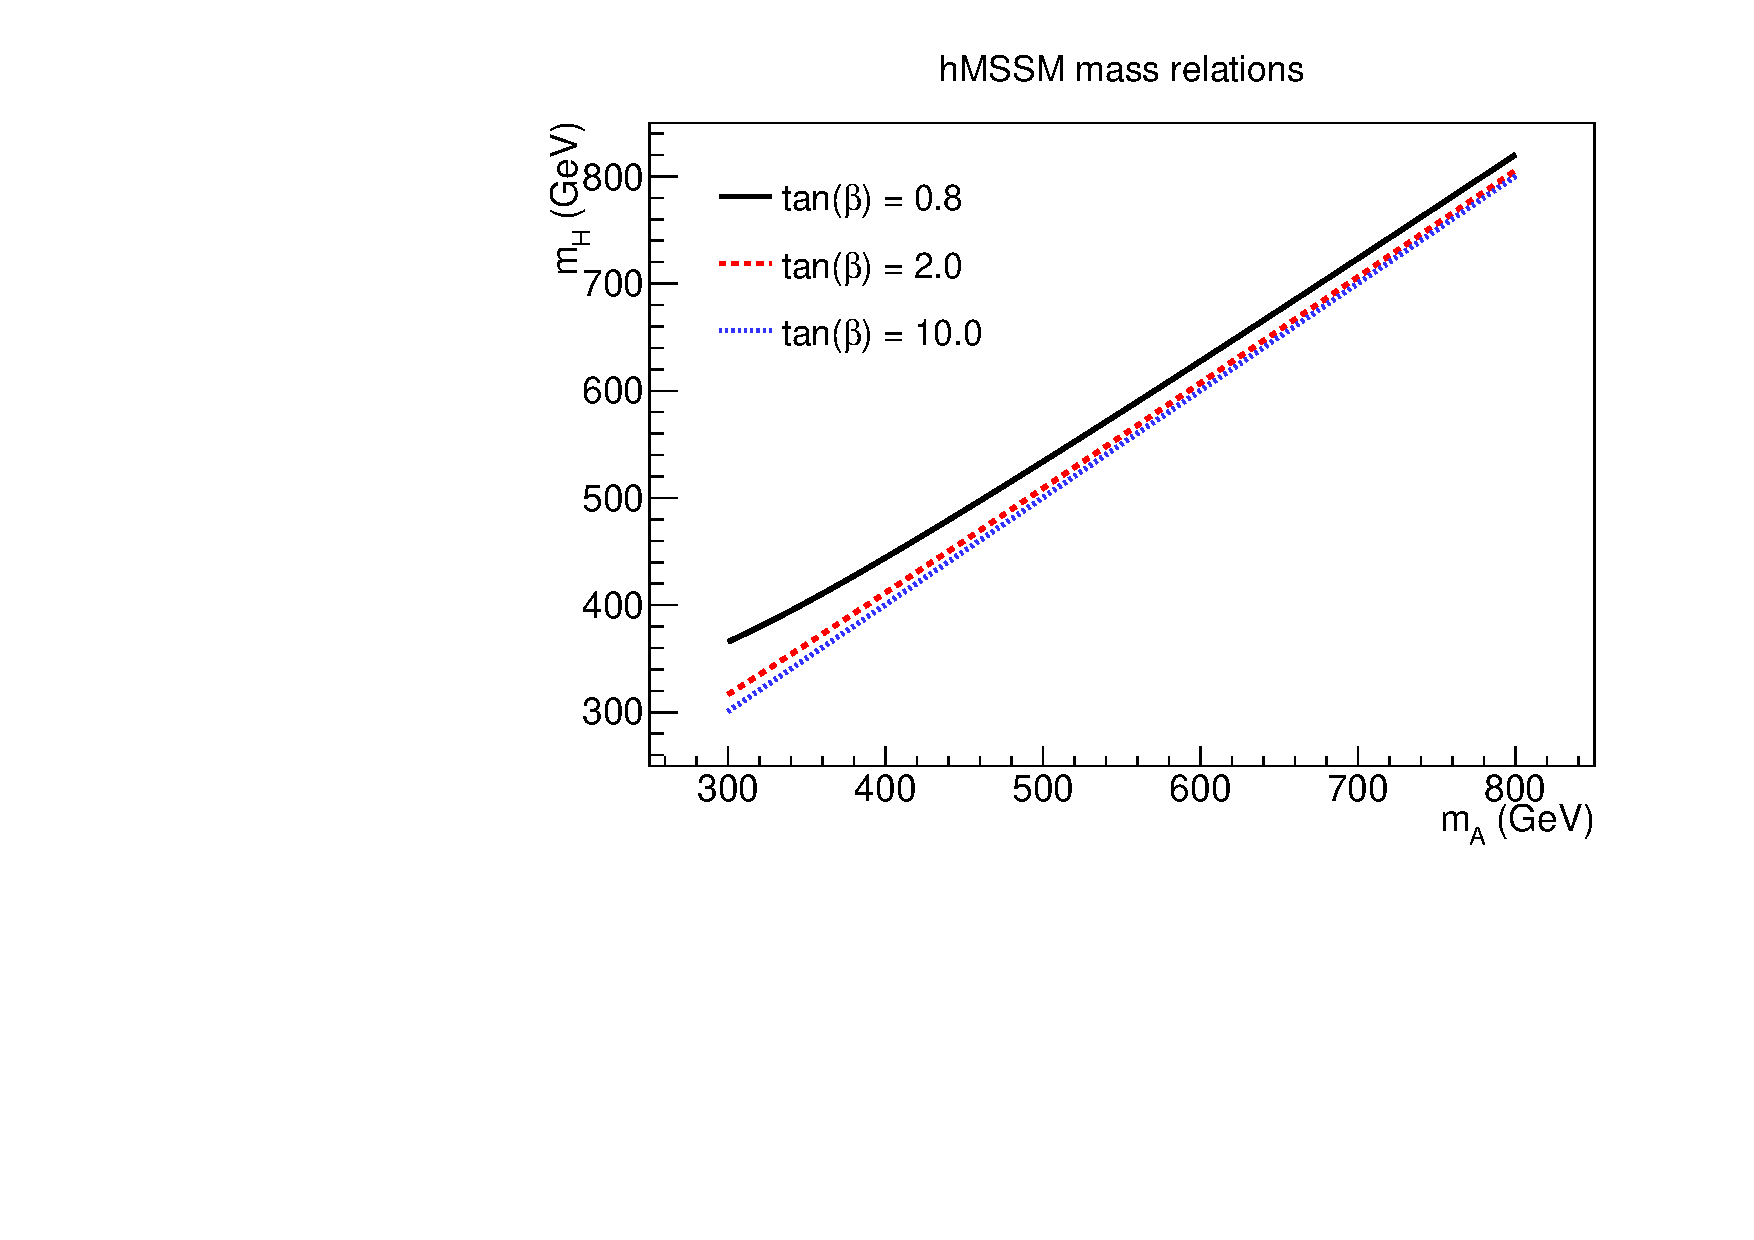
\includegraphics[width=0.8\textwidth,keepaspectratio=true]{fig/chapt8/hmssm/mh_vs_ma.pdf}
\caption{Scalar mass ($m_\mathrm{H}$) as a function of pseudoscalar mass ($m_\mathrm{A}$) for different values of $\tan\beta$ in the hMSSM.}
\label{fig:hmssm_mass_relations}
\end{figure}

Under the assumption that new particles do not affect the production and decay of the Higgs bosons considered, the discussion in this section applies equally to the hMSSM and to generic type-2 2HDM models.
The major exception is that MSSM models lead to strict mass relations between the additional Higgs bosons for a given $\tan\beta$.
Figure~\ref{fig:hmssm_mass_relations} shows the dependence of the scalar mass on the pseudoscalar mass for different values of $\tan\beta$\footnote{This plot and the following plots in this subsection are made using the publicly available hMSSM model files~\cite{LHCHXSWGMSSM}, as discussed in reference~\cite{deFlorian:2016spz}. For the final interpretation, we use a finer grid for the predictions, which we needed to recalculated. The details are given in the next subsection.}. While for high $\tan\beta$, the $A$ and $H$ masses are nearly degenerate, the $H$ mass is significantly larger for $\tan\beta$ near 1 and below.
This implies that the presented search cannot use the often-made assumption of mass degeneracy between the $H$ and $A$, but needs to consider the $H$ mass for each point in the $(m_A, \tan\beta)$ plane.

\begin{figure}[!Hhtb]
\centering
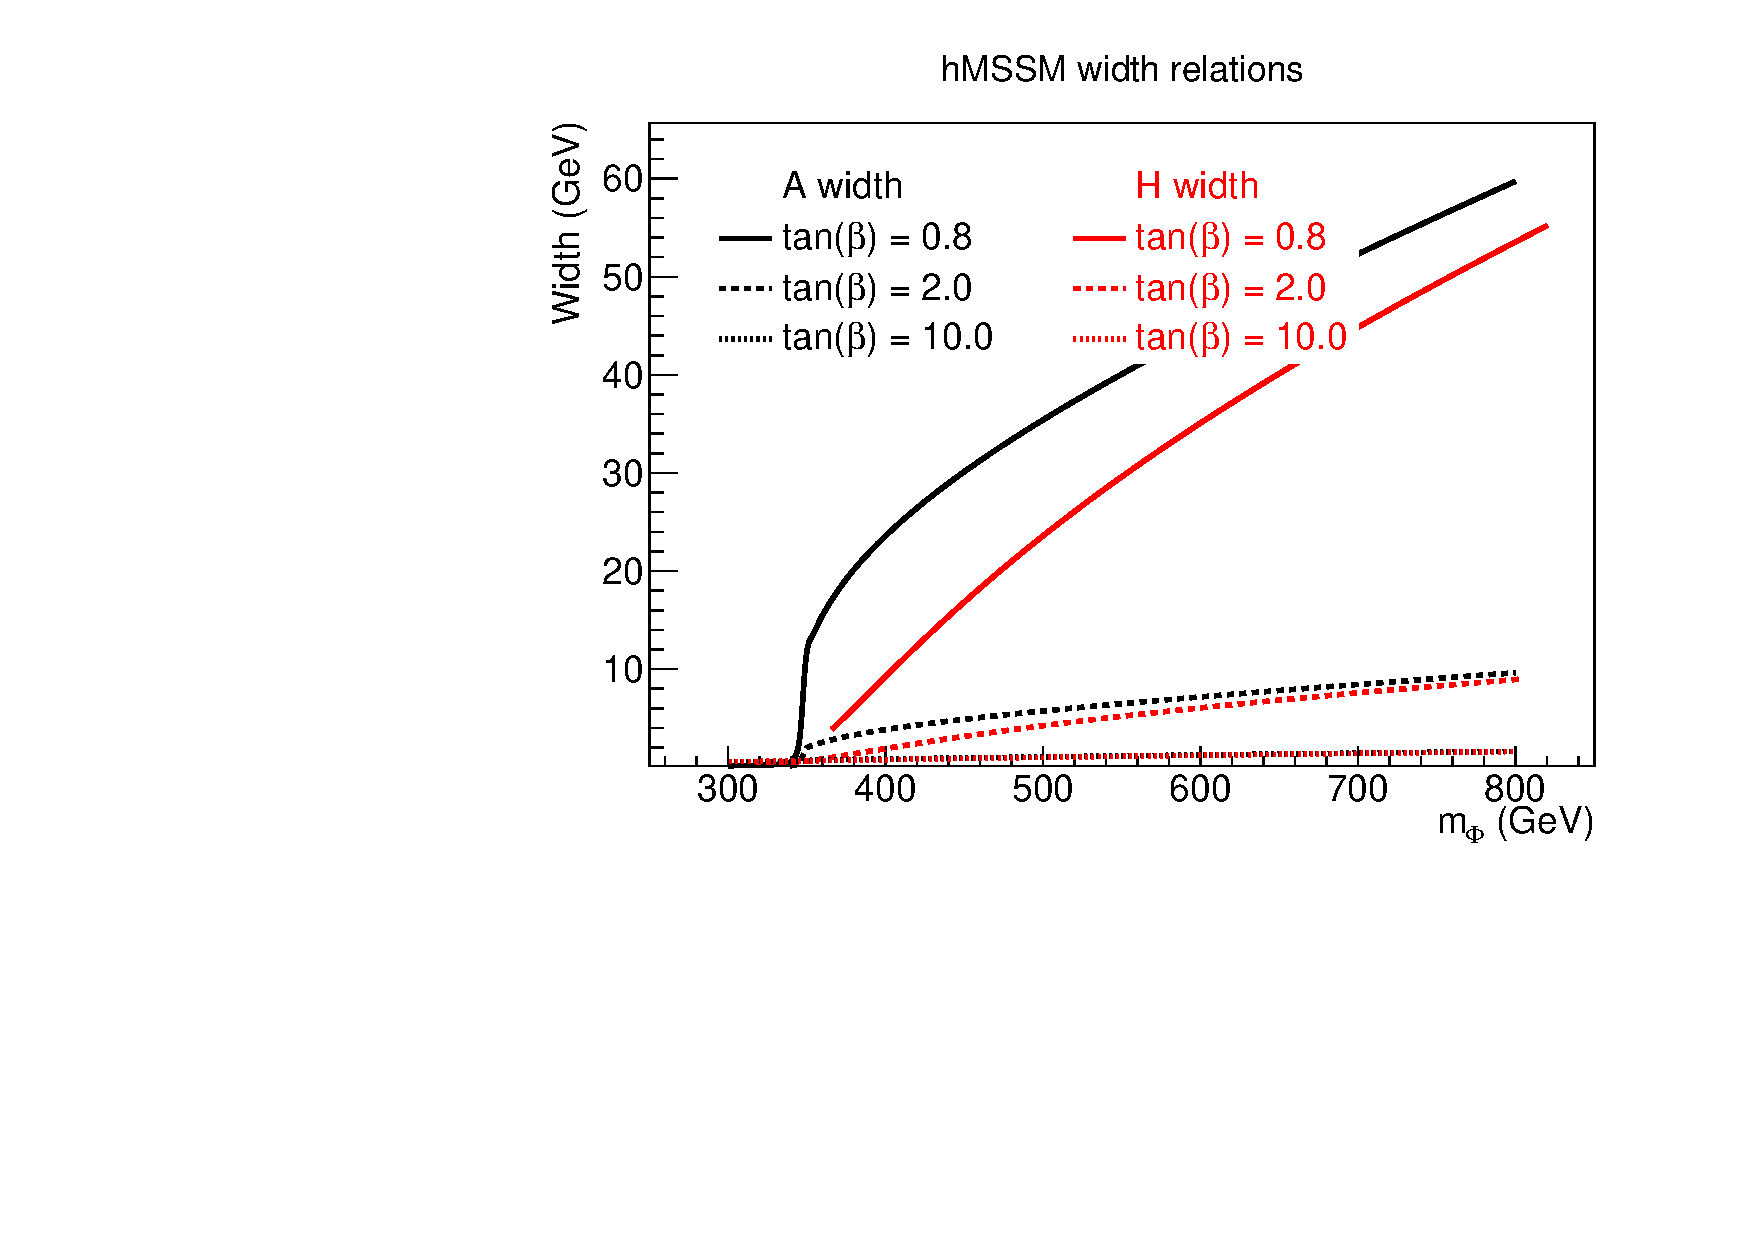
\includegraphics[width=0.8\textwidth,keepaspectratio=true]{fig/chapt8/hmssm/widths_vs_ma.pdf}
\caption{Scalar (red) and pseudoscalar (black) total widths as a function of corresponding mass ($m_\mathrm{\Phi}$) for different values of $\tan\beta$ in the hMSSM.}
\label{fig:hmssm_width_relations}
\end{figure}

Figure~\ref{fig:hmssm_width_relations} shows the $A$ and $H$ widths as a function of the corresponding mass for different values of $\tan\beta$.

\begin{figure}[!Hhtb]
\centering
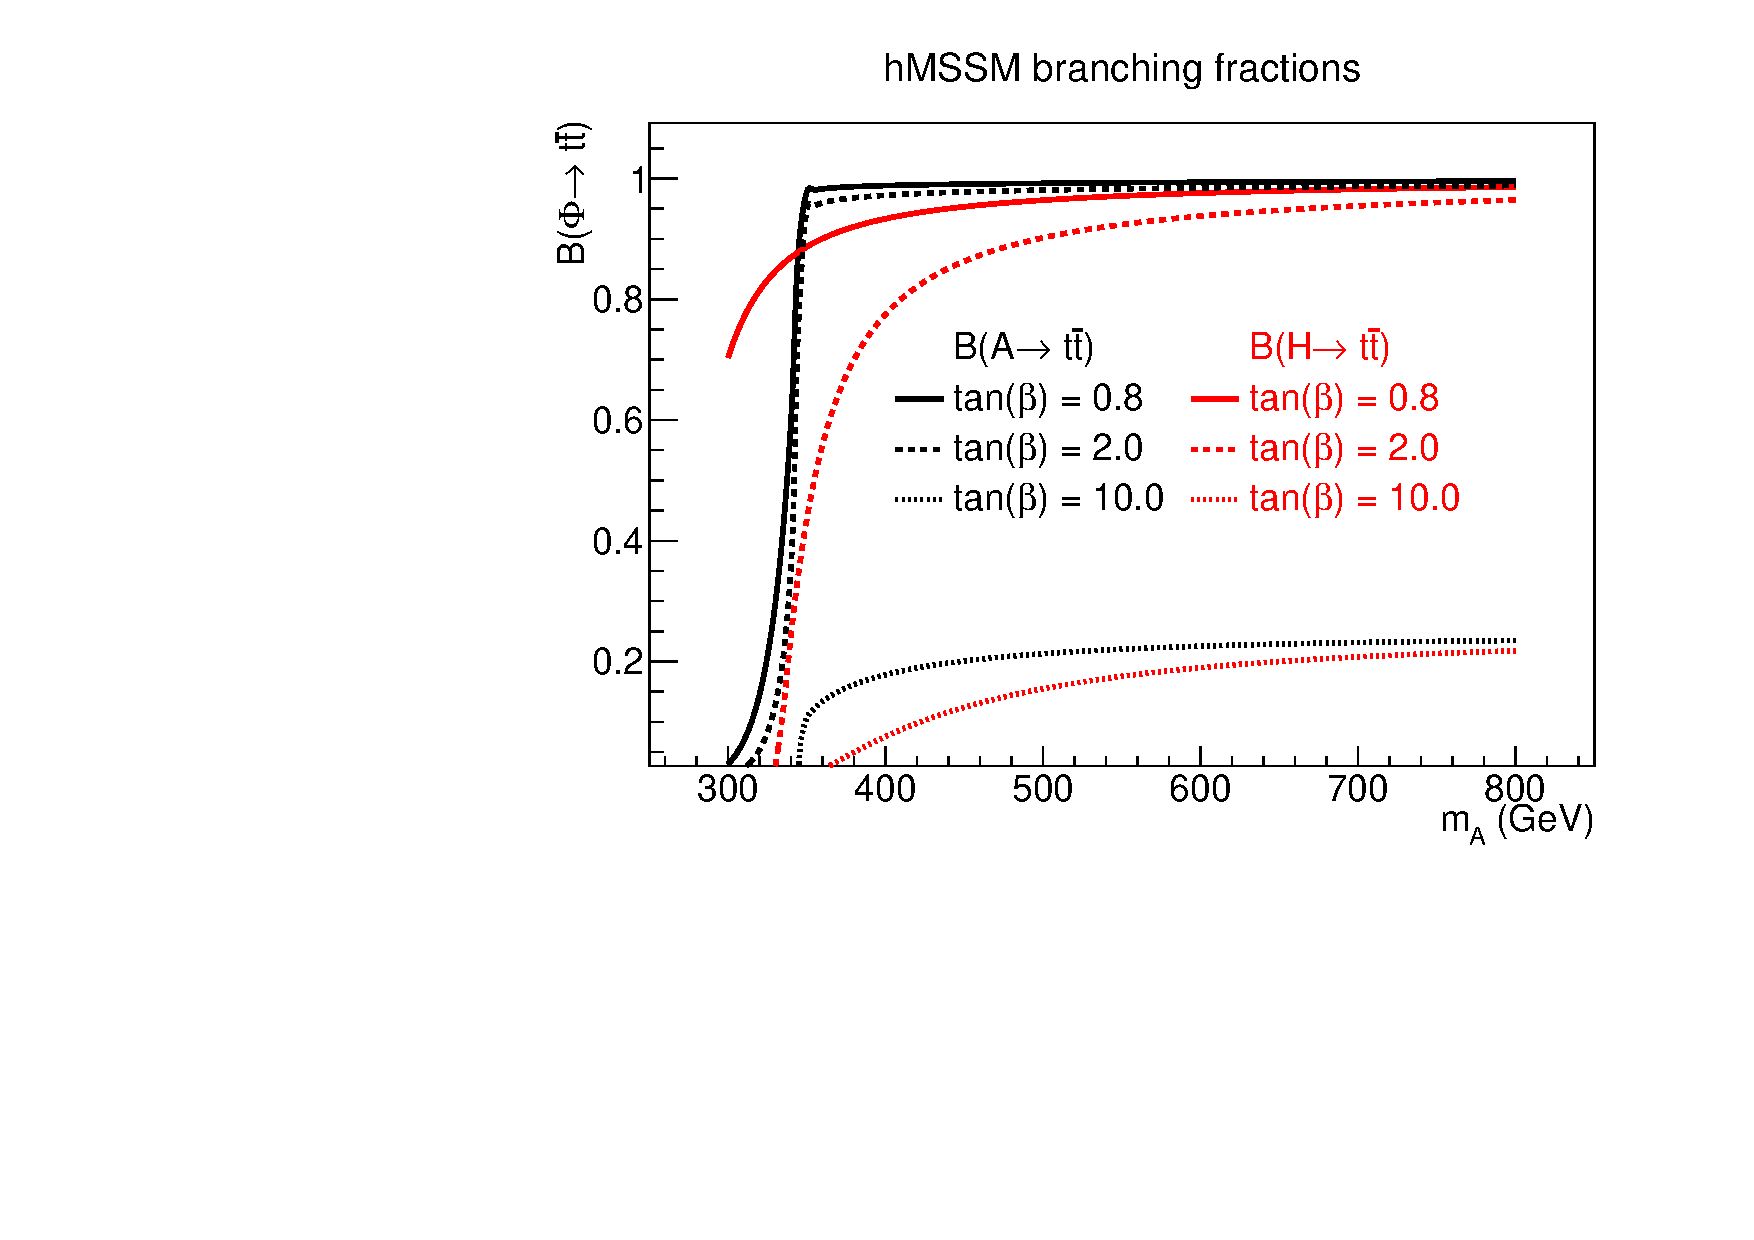
\includegraphics[width=0.8\textwidth,keepaspectratio=true]{fig/chapt8/hmssm/btt_vs_ma.pdf}
\caption{Branching fraction for scalar (red) and pseudoscalar (black) decays to $t\bar t$ as a function of pseudoscalar mass ($m_\mathrm{A}$) for different values of $\tan\beta$ in the hMSSM.}
\label{fig:hmssm_branching}
\end{figure}

The branching fractions for $A$ and $H$ decays to $t\bar t$ are given in Fig.~\ref{fig:hmssm_branching}.
For $A$ decays, the branching fraction is close to unity for small values of $\tan\beta$.
For $H$ decays, the branching fraction is still close to unity but a bit smaller because of additional open decay channels including bosons.
\begin{figure}[!Hhtb]
\centering
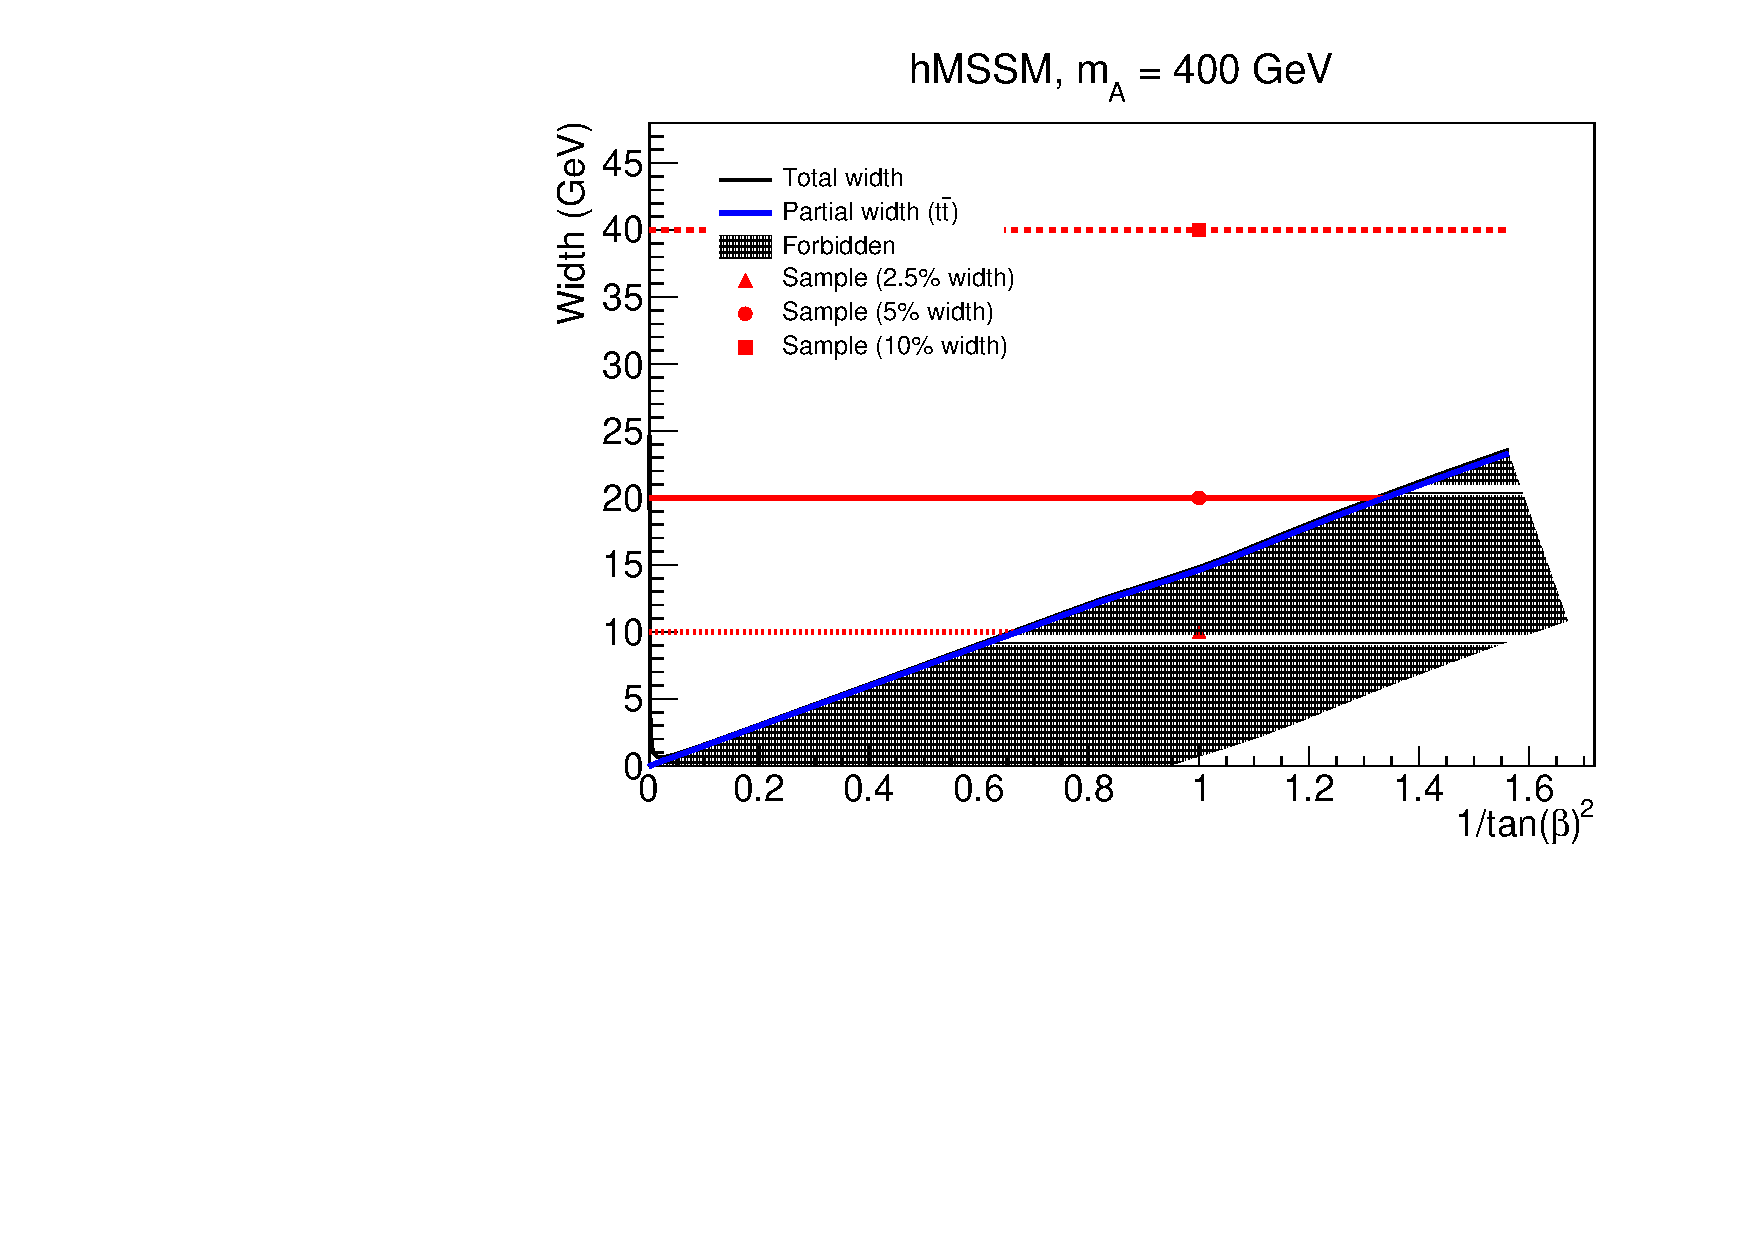
\includegraphics[width=0.45\textwidth,keepaspectratio=true]{fig/chapt8/hmssm/width_vs_tanb_mA400.pdf}
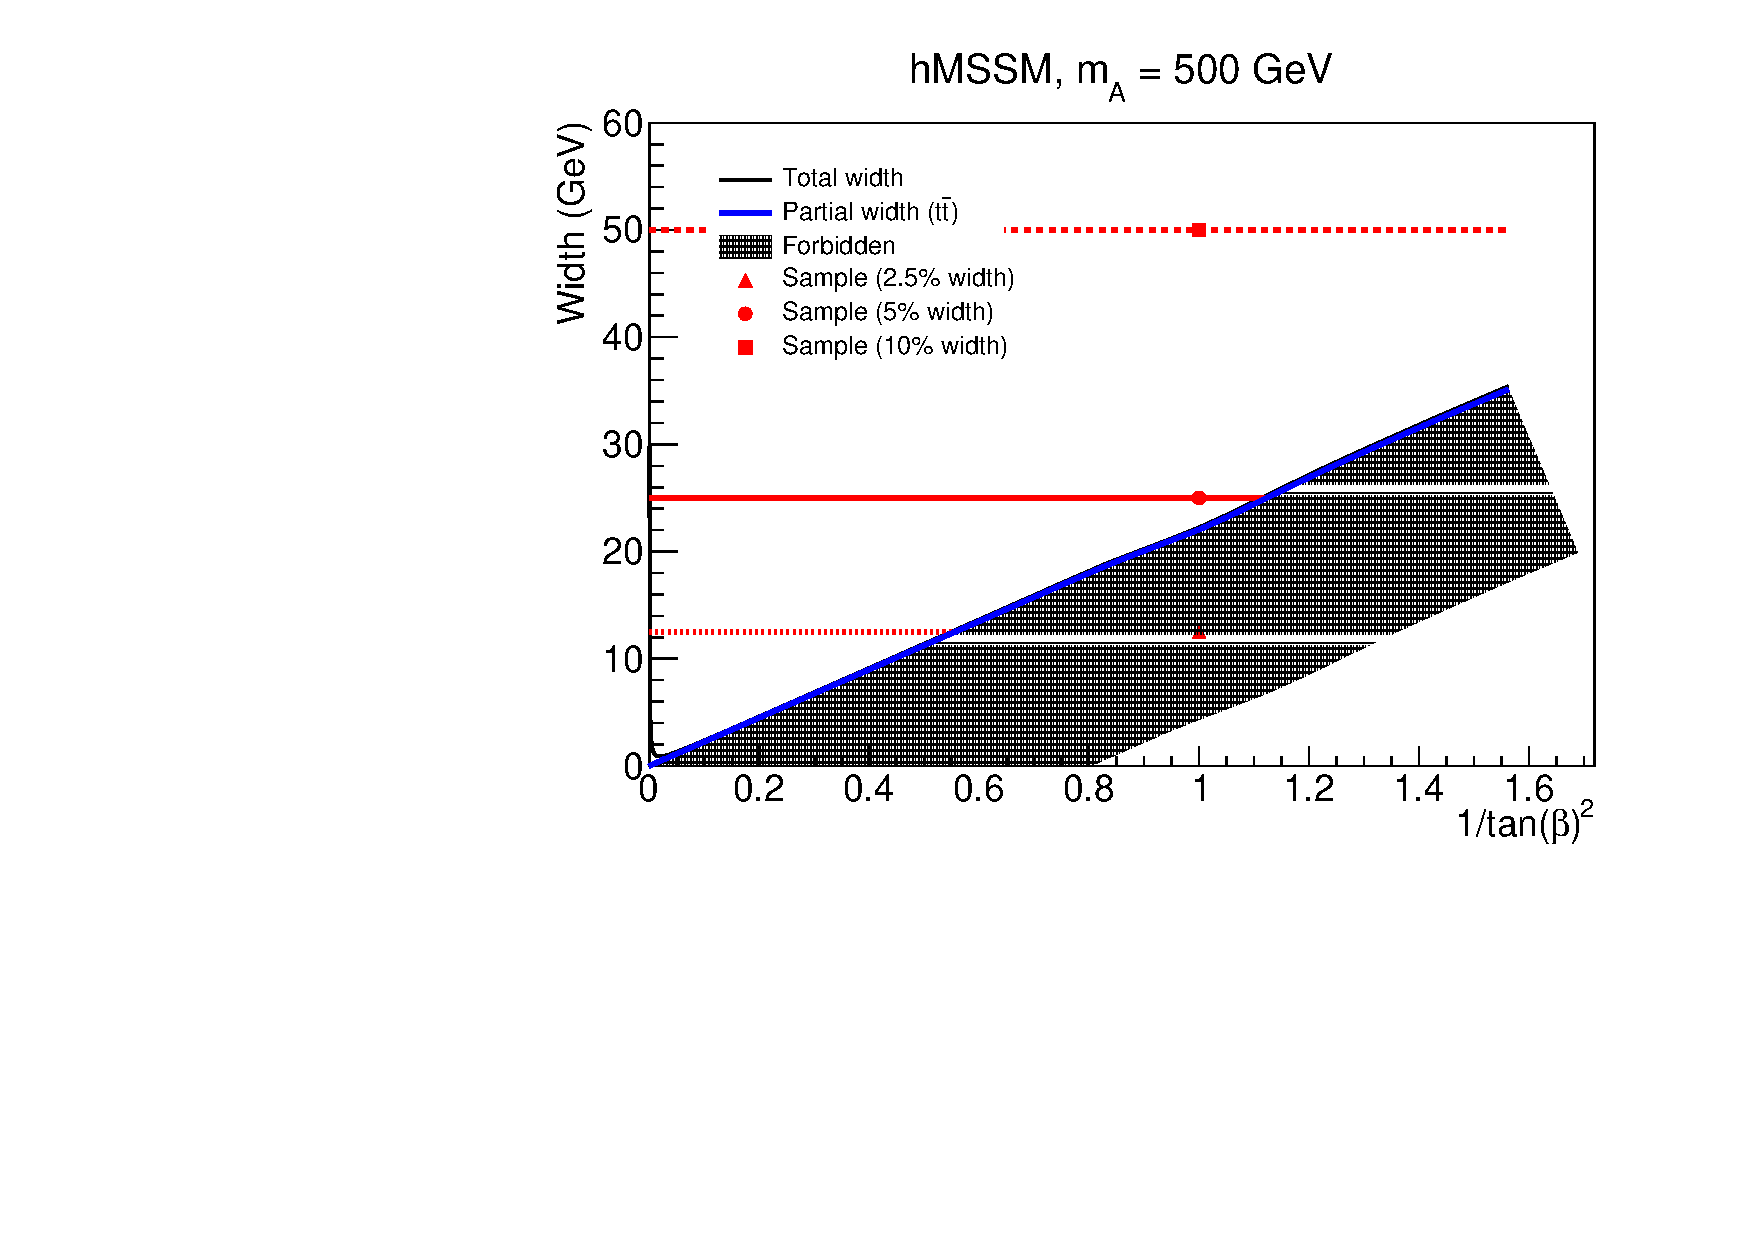
\includegraphics[width=0.45\textwidth,keepaspectratio=true]{fig/chapt8/hmssm/width_vs_tanb_mA500.pdf}
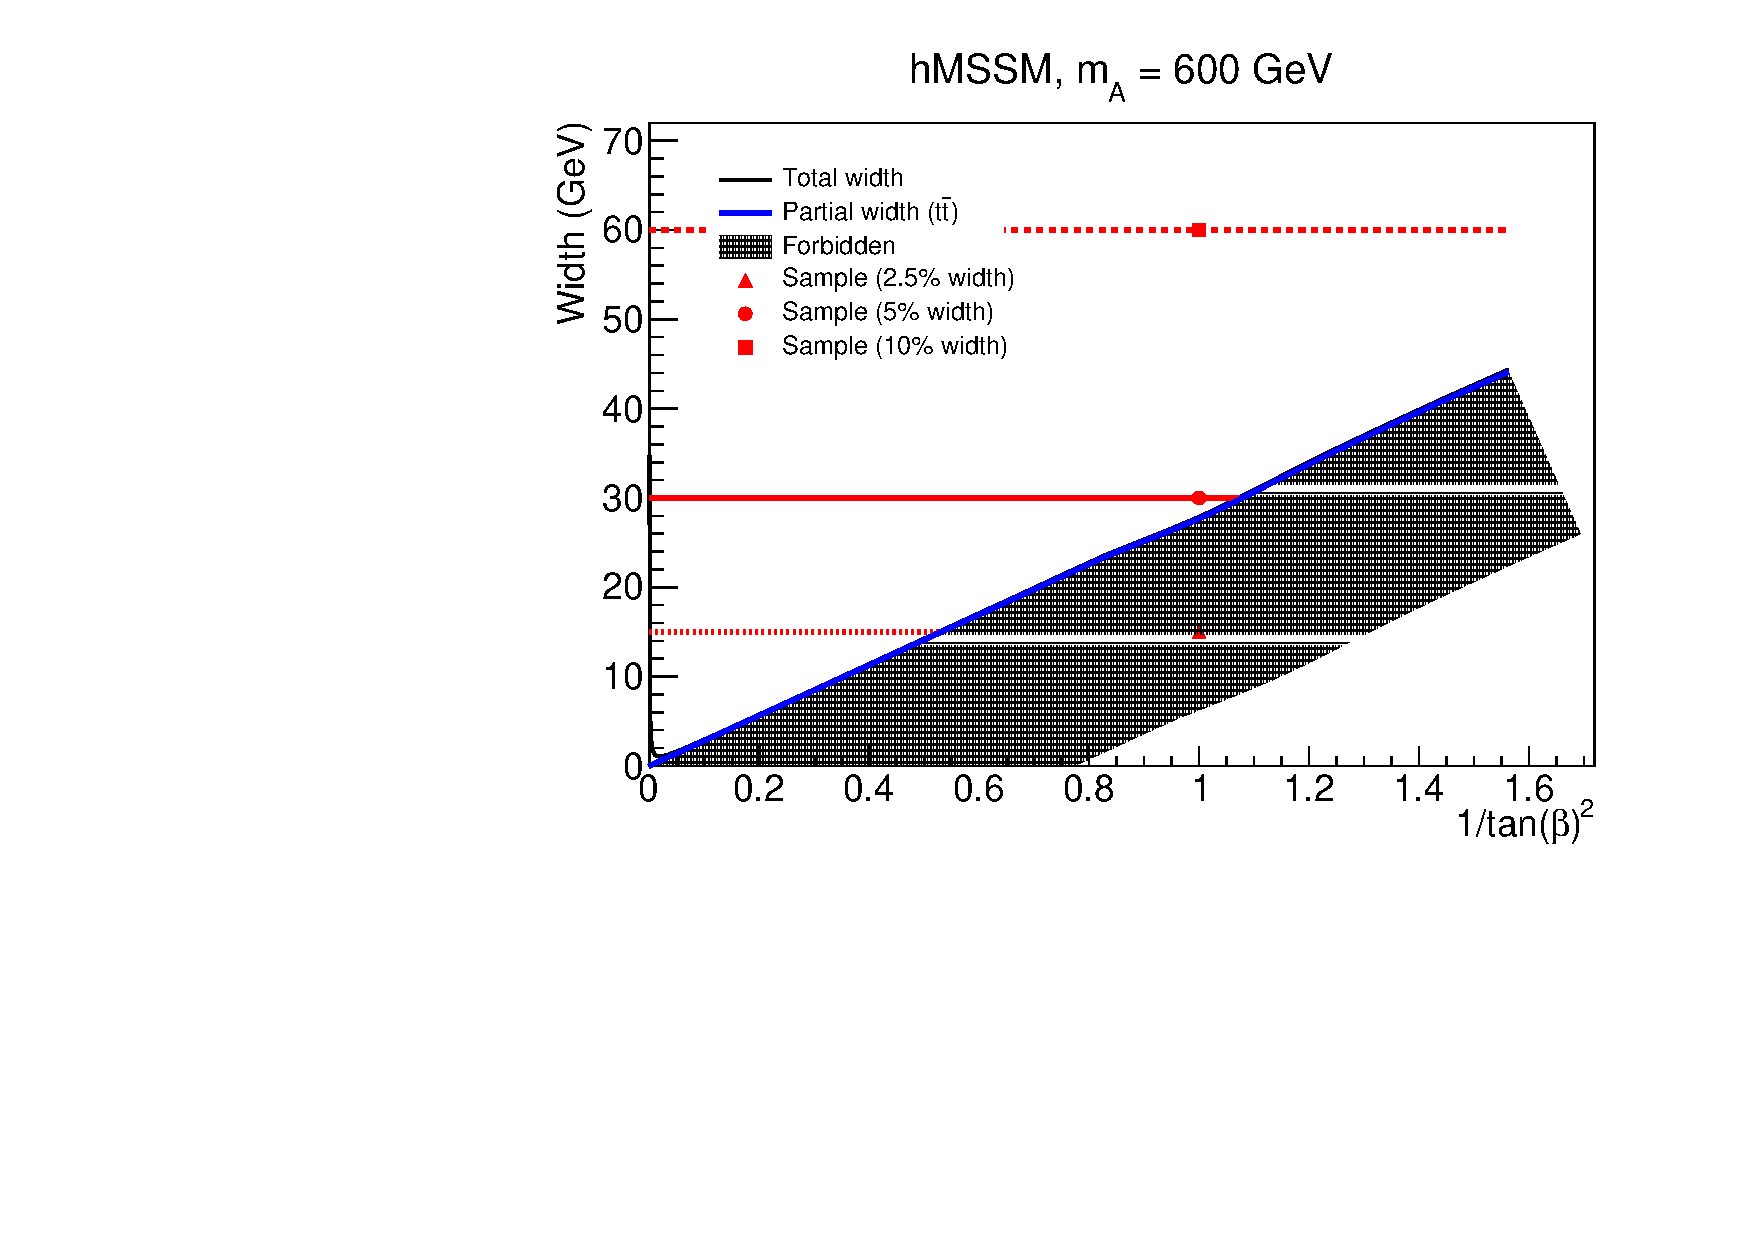
\includegraphics[width=0.45\textwidth,keepaspectratio=true]{fig/chapt8/hmssm/width_vs_tanb_mA600.pdf}
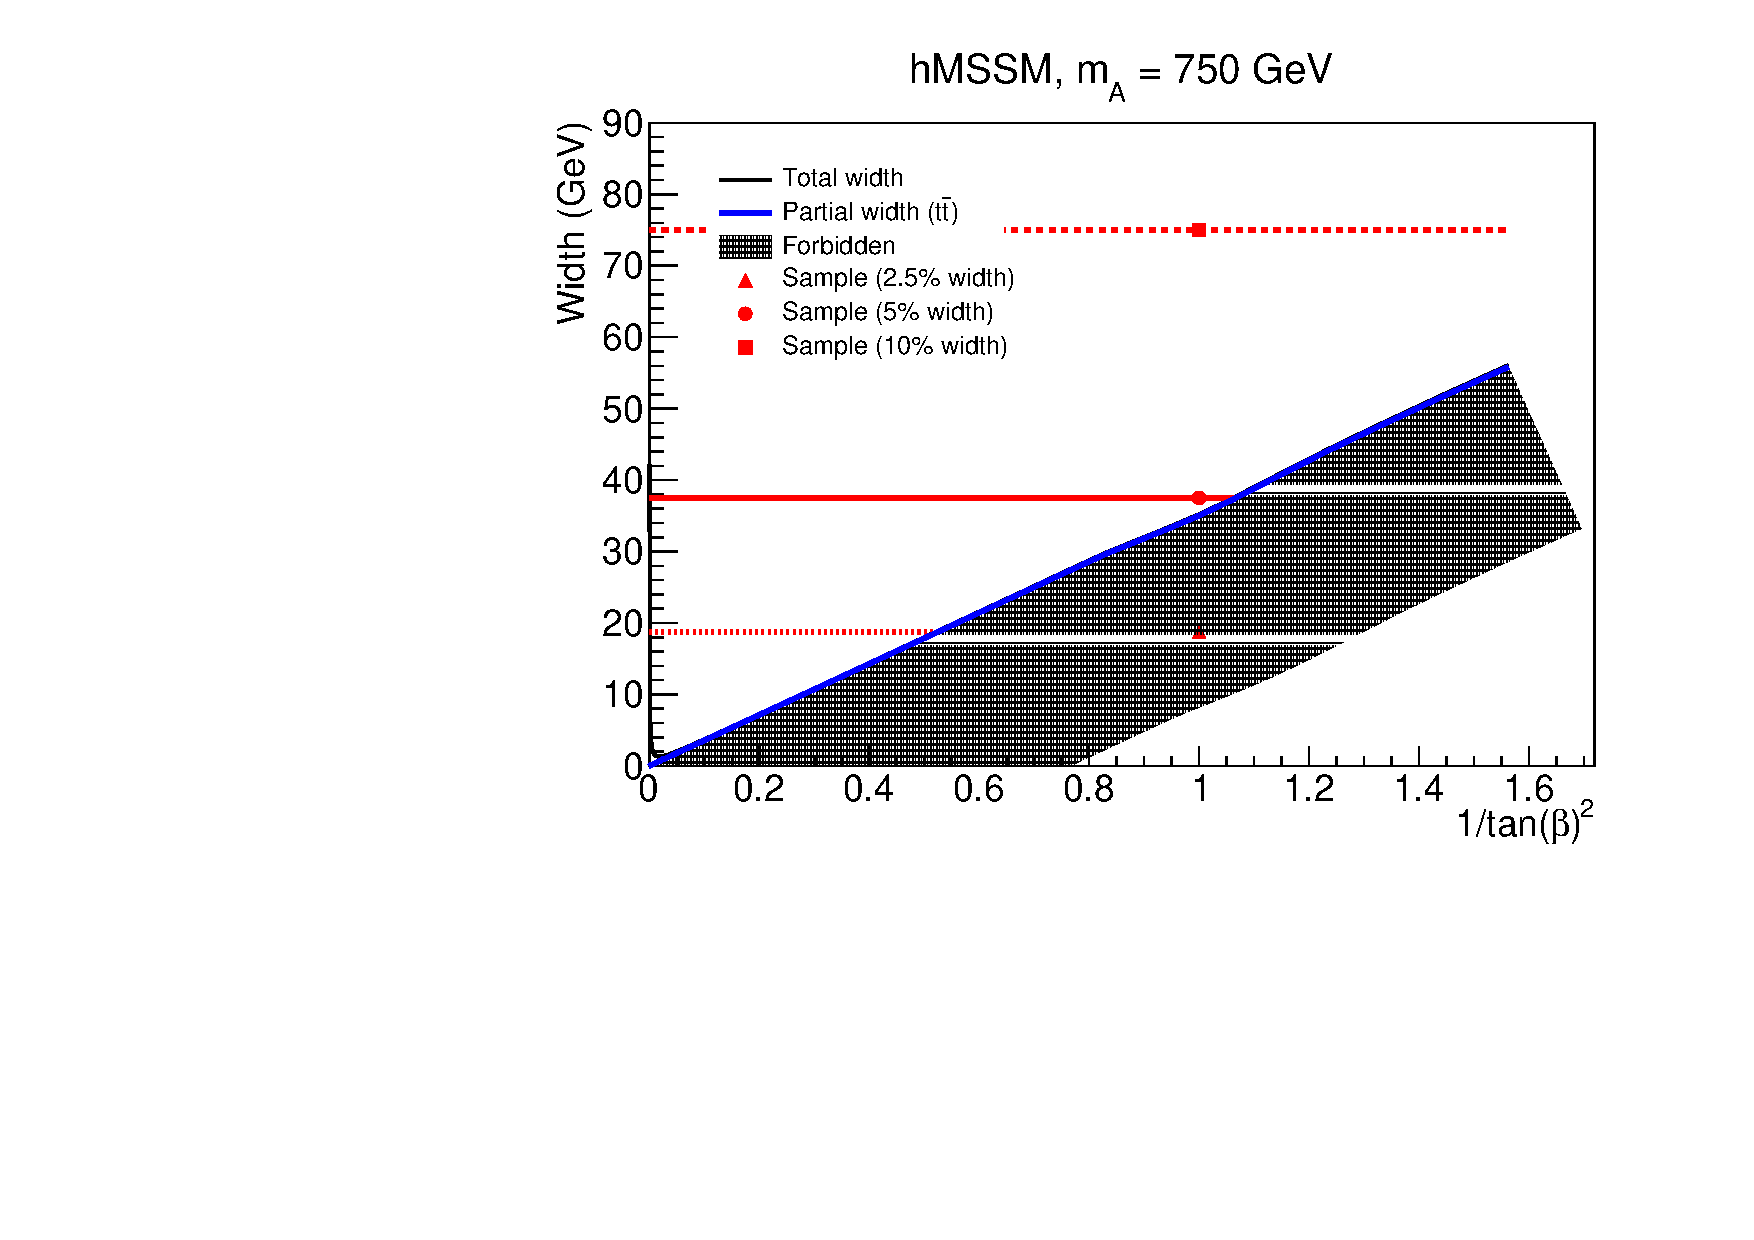
\includegraphics[width=0.45\textwidth,keepaspectratio=true]{fig/chapt8/hmssm/width_vs_tanb_mA750.pdf}
\caption{Total width of pseudoscalar in the hMSSM (black line) and partial width for decays to $t\bar t$ as a function of $1/\tan\beta^2$. In the forbidden region (shown in grey), the total width would be smaller than the partial width for decays to $t\bar t$. In addition, the three widths for which samples are produced are indicated as horizontal lines. In addition, their default configuration with $g=1$, corresponding to $\tan\beta = 1$, is shown by the markers. The horizontal line indicates the phase space that is covered by varying the coupling $g$, and hence the rates of the signal and interference contributions. For a given sample, a specific point in the hMSSM, which can be obtained from the black curve, can be excluded if the observed limit on the coupling modifier g is larger than the corresponding $\tan\beta$ value. These relations are shown for masses of 400, 500, 600, and 750\,GeV.}
\label{fig:width_vs_tanb}
\end{figure}

Finally, Fig.~\ref{fig:width_vs_tanb} shows the plane of pseudoscalar width vs.\ $1/(\tan\beta)^2$, with the latter being equivalent to the coupling squared, $g^2$.
The total width increases roughly linearly with $g^2$ where the decay to $t\bar t$ dominates.
Also shown are the three produced samples at relative widths of 2.5, 5, and 10\%, with the markers corresponding to $\tan\beta = 1$ or, equivalently, $g = 1$, and the attached lines showing the variation when the coupling is altered.
For a given width, limits can be set on given points in the hMSSM by checking whether the observed upper limit on the coupling is smaller than the coupling that corresponds to the $\tan\beta$ at the given width.
To cover sufficiently small variations in $\tan\beta$, the produced widths are evidently not sufficient.
Therefore, an interpolation of the produced samples is applied as well as an extrapolation to lower widths, using the narrow-width approximation.
Details on these procedures are given in Sec.~\ref{sec:morphing}.

\subsection{Higher-order cross sections}

Cross section calculations with NNLO accuracy are available for $gg\rightarrow A$ and $gg\rightarrow H$ production, and recommended to be used by relevant LHC searches (see in particular the yellow report 4~\cite{deFlorian:2016spz}).
We scale the resonant part of the signal with the ratio of NNLO to LO cross sections for $gg\rightarrow A$ or $gg\rightarrow H$ production, respectively.
We define this ratio as $r_\text{S}$.
In line with the 8\,TeV ATLAS result~\cite{Hespel:2016qaf,PhysRevLett.119.191803}, we scale the yields of the interference between $gg\rightarrow A$ or $gg\rightarrow H$ signal and the SM $t\bar t$ background with

\begin{equation}
k = \sqrt{r_\text{S} r_{SM t\bar t}},
\end{equation}

with $r_{SM t\bar t}$ denoting the ratio of the SM $t\bar t$ cross section at NNLO+NNLL and LO accuracy.

The signal cross sections are obtained in the following way.
First, the hMSSM parameters (in particular masses and widths of the additional Higgs bosons) are obtained with the \textsc{2HDMC} programme~\cite{2hdmc}
Then, the cross sections at NNLO accuracy are obtained with the \textsc{SusHi} programme~\cite{sushi}.
These cross sections are obtained with the same setup as the results in reference~\cite{deFlorian:2016spz}.
The numerical values of the parameters can be found in reference~\cite{LHCHXSWGMSSM}.
The only difference is that we use a different PDF set, \textsc{NNPDF} with version 3.0, to correspond to the PDF set that is used in the production of our signal and background samples.

The LO cross sections are calculated separately both with the \textsc{MadGraph} programme and with \textsc{SusHi}. The obtained cross sections are found to be consistent within 1\%.
The ratios of NNLO and LO cross sections show a slight dependence on mass and width, and are typically of the order of 2. Finally, we scale the cross sections obtained by \textsc{MadGraph} with the ratio of the NNLO and LO cross sections obtained with \textsc{SusHi}.

For $t\bar t$ production, we use the \textsc{Top++}~\cite{Czakon:top_pp} programme to calculate cross sections both at NNLO+NNLL and at LO accuracy.
We also calculate the LO cross section with the \textsc{MadGraph} event generator used for our signal sample production.
The LO cross sections obtained with \textsc{Top++} and \textsc{MadGraph} agree at the per mill level.
The ratio of NNLO+NNLL and LO cross sections is found to be 1.57.
\begin{figure}[!Hhtb]
\centering
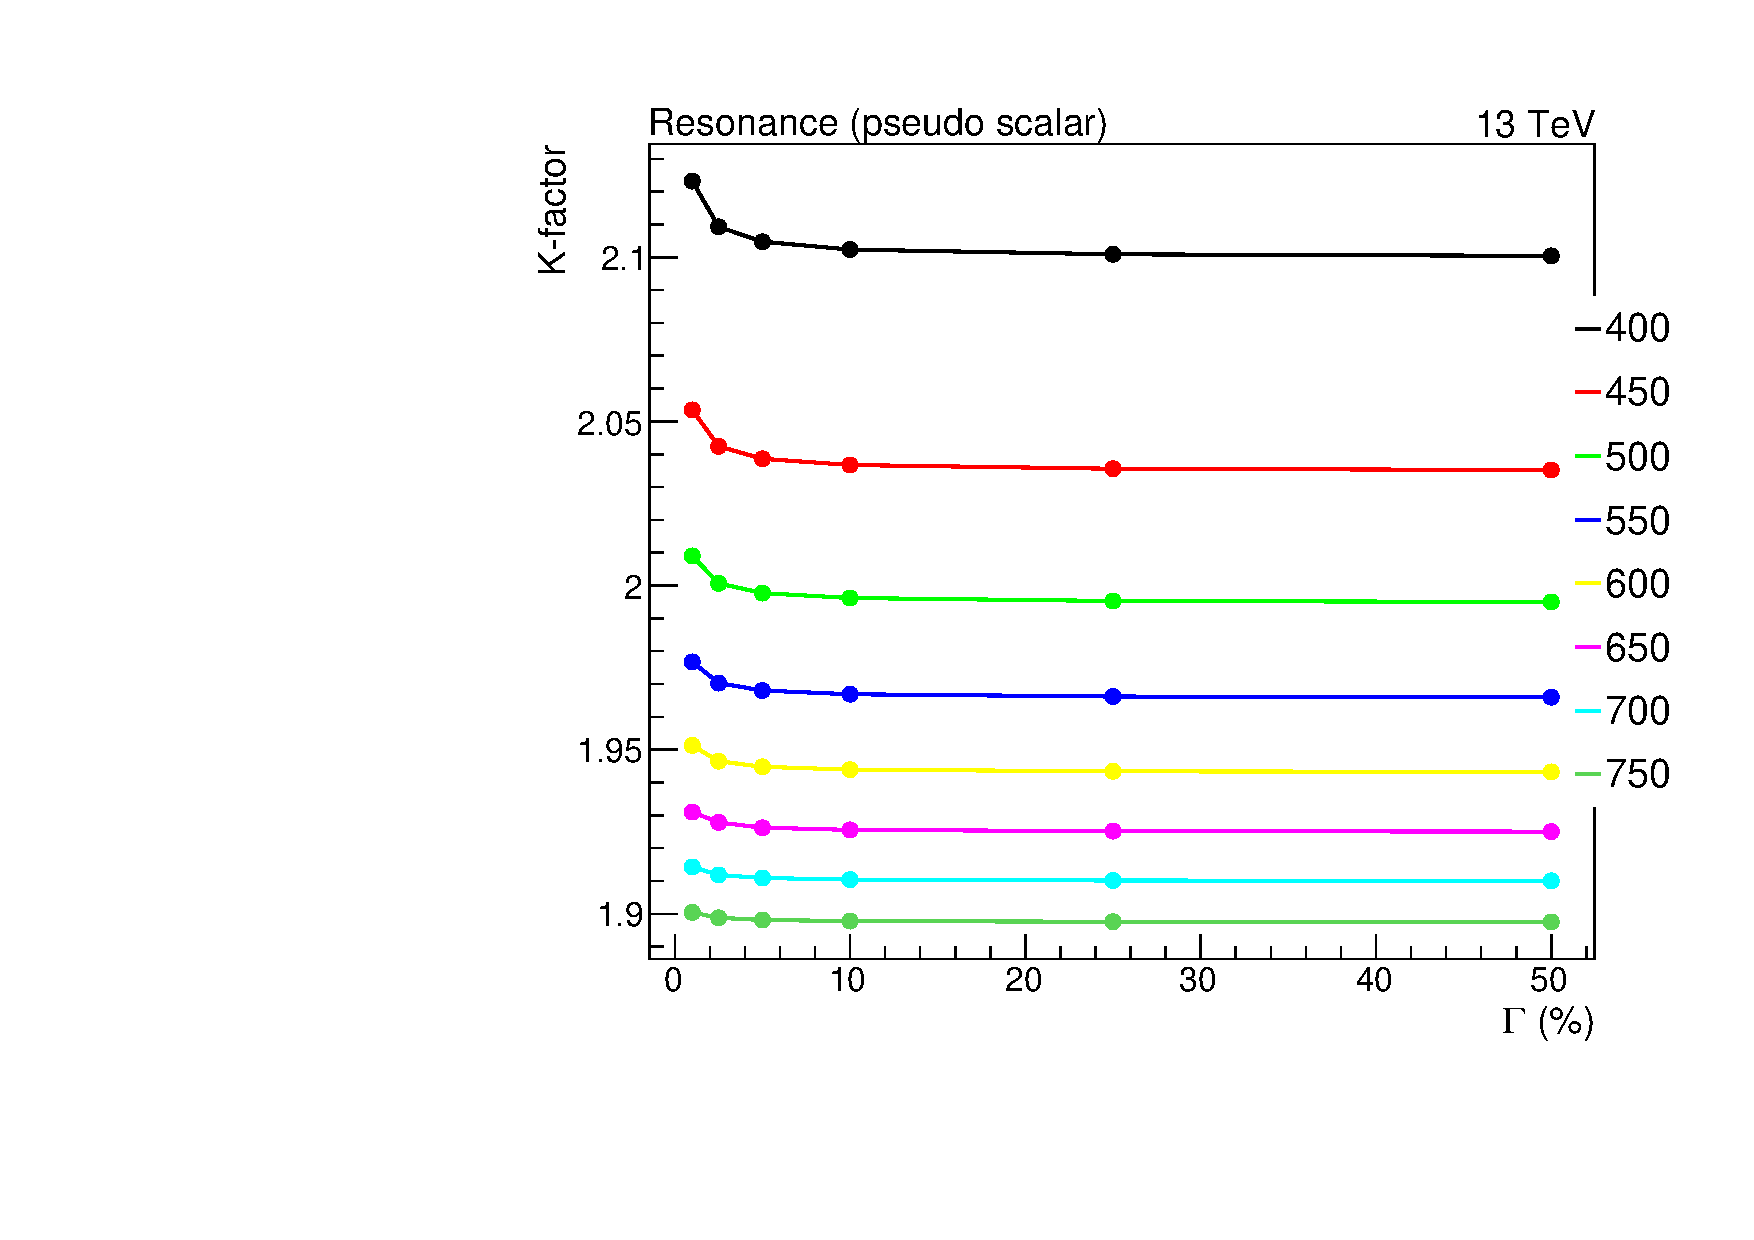
\includegraphics[width=0.45\textwidth,keepaspectratio=true]{fig/chapt8//kfactors/k_factor_PScalar_res.pdf}
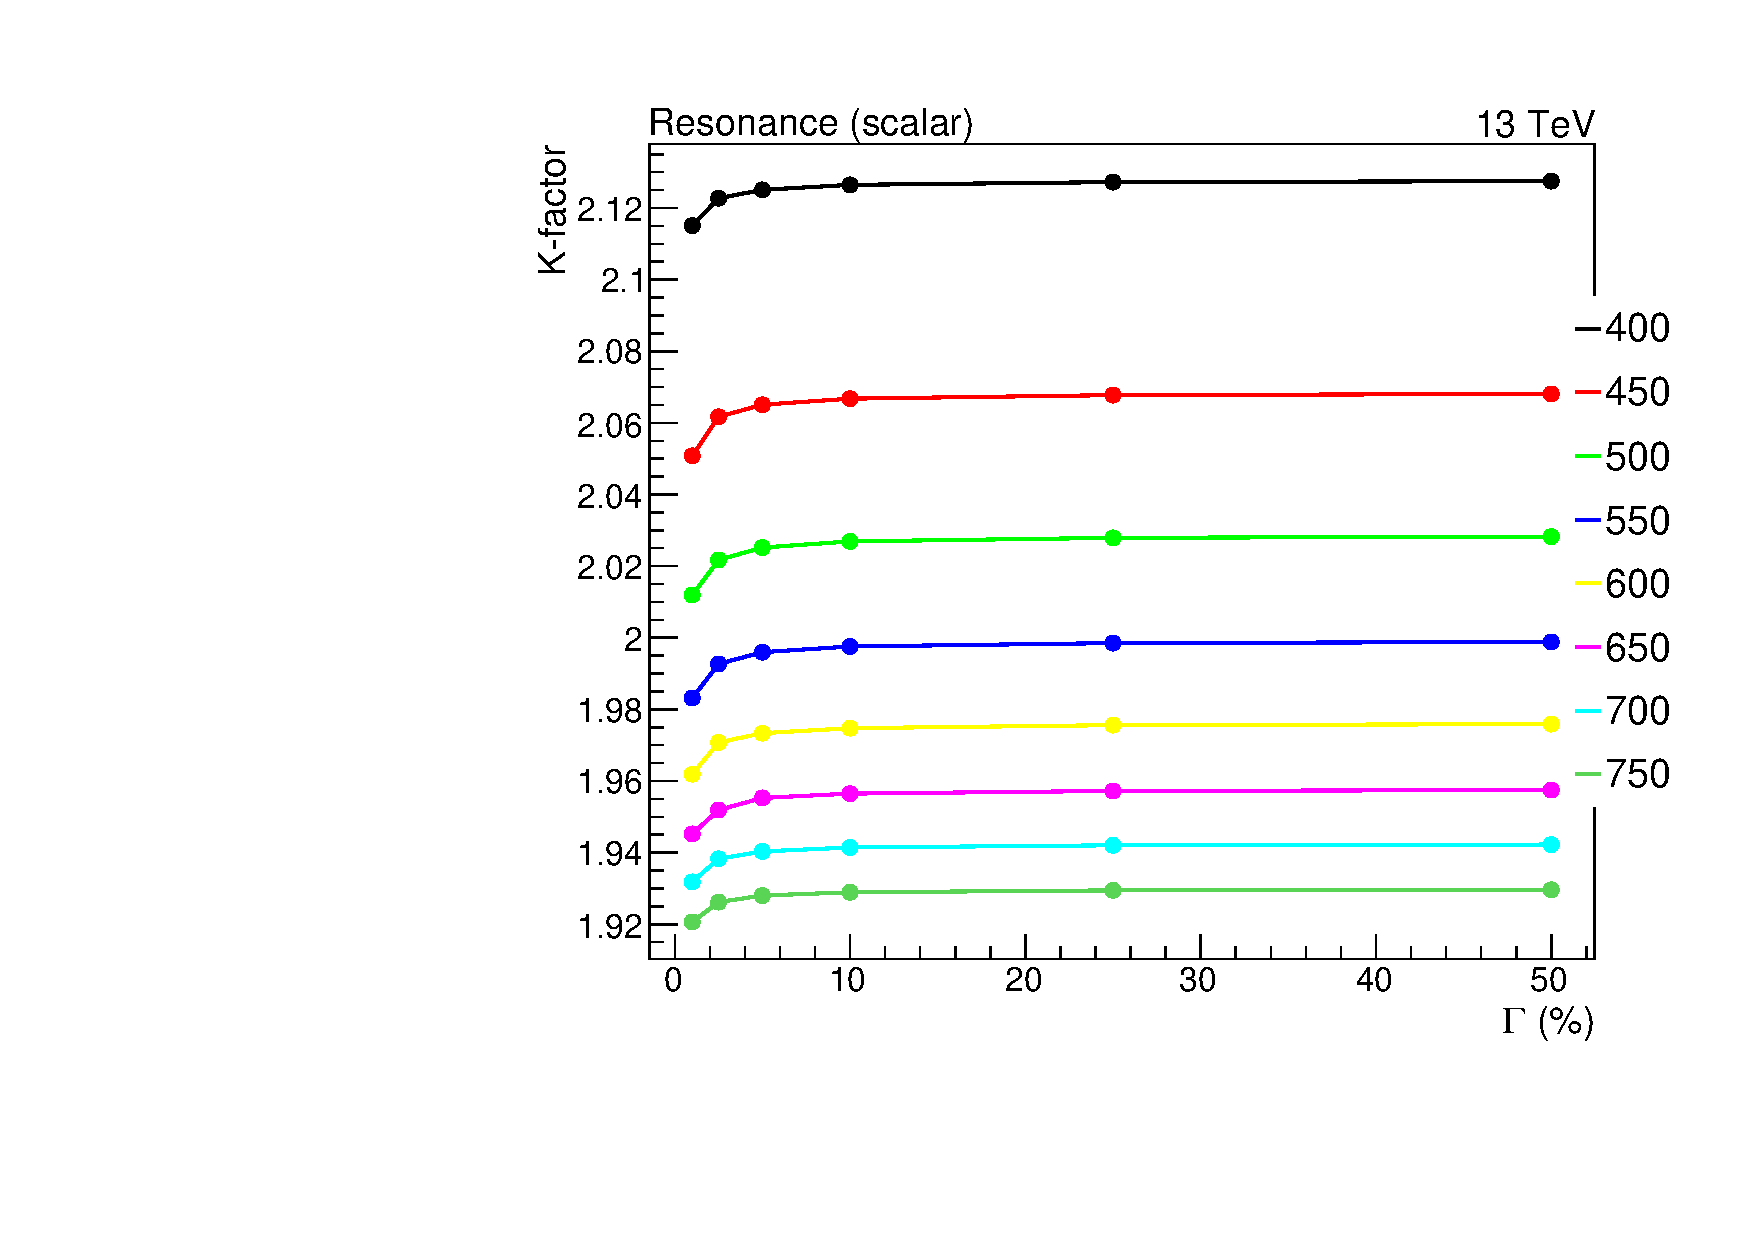
\includegraphics[width=0.45\textwidth,keepaspectratio=true]{fig/chapt8//kfactors/k_factor_Scalar_res.pdf}
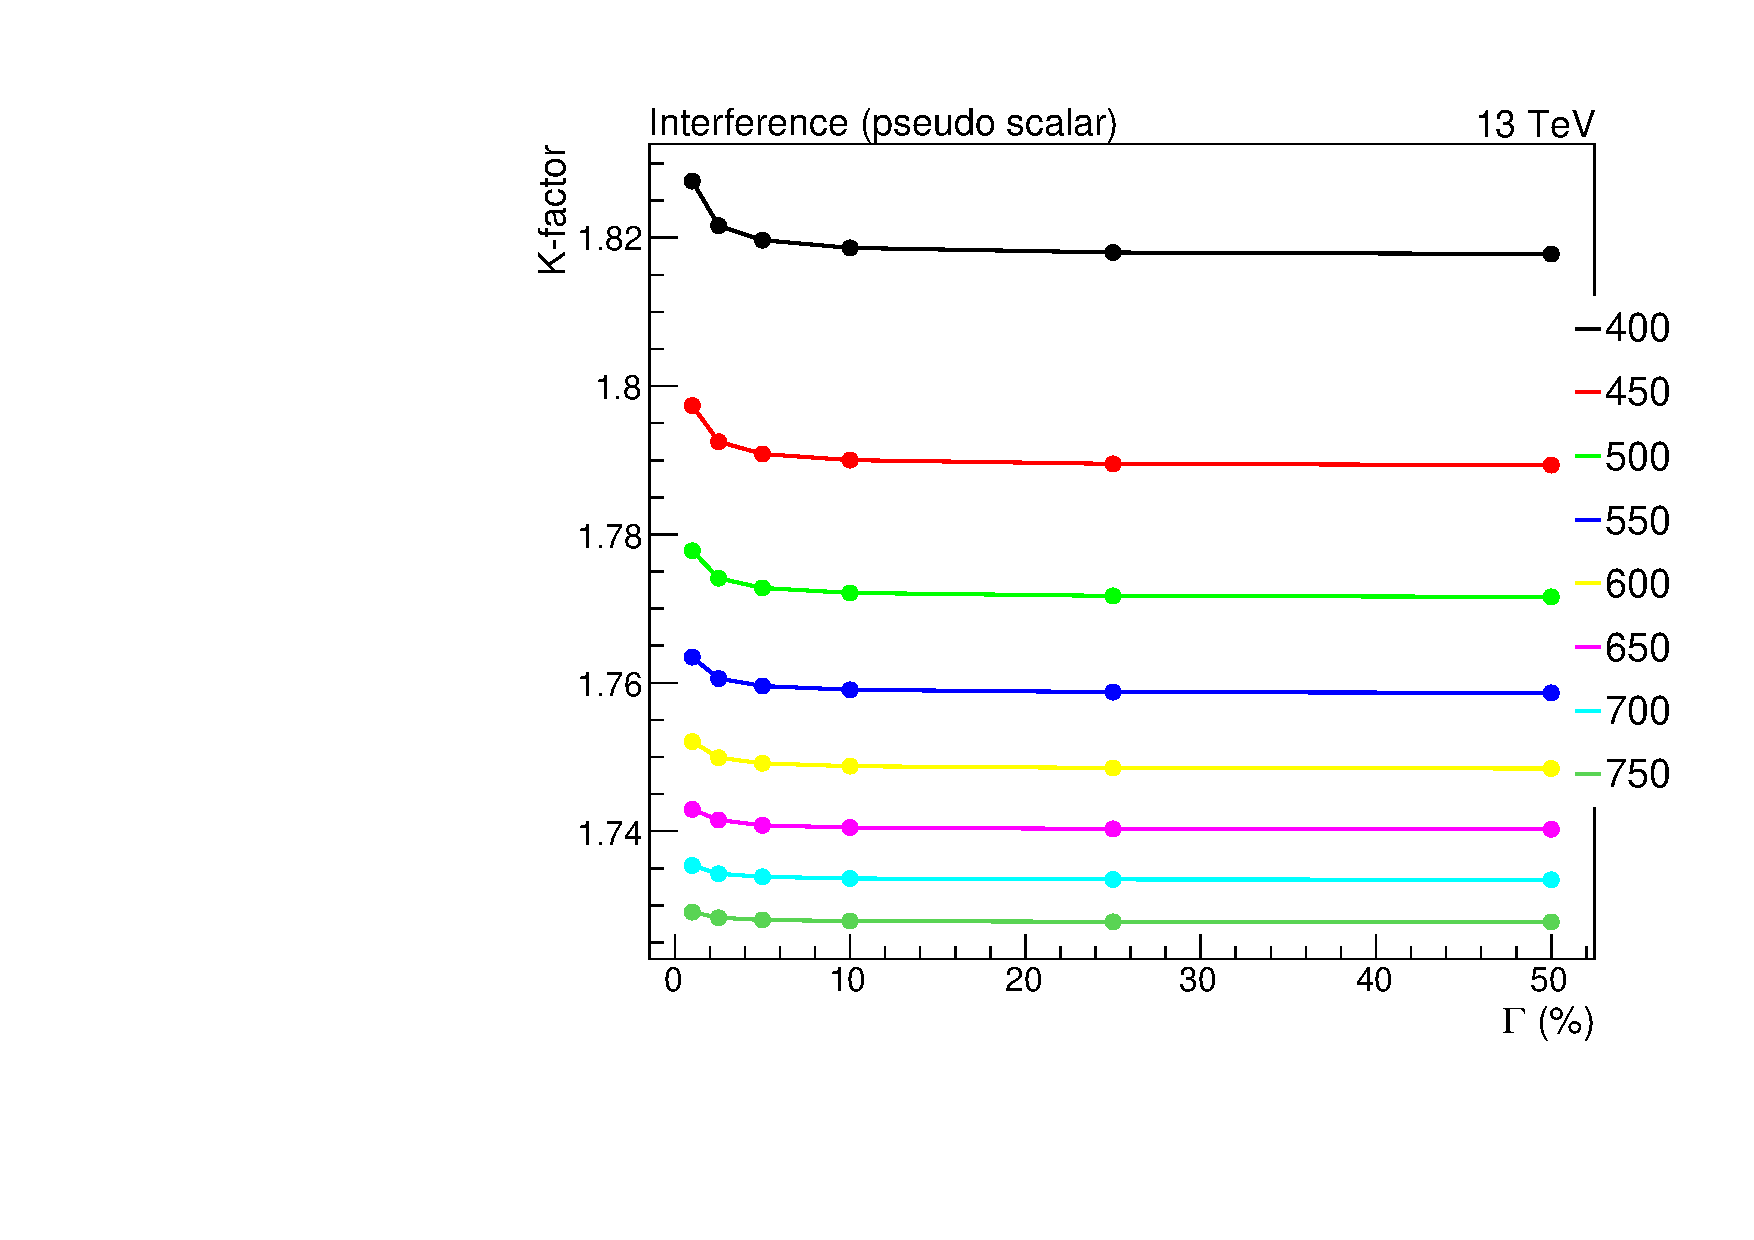
\includegraphics[width=0.45\textwidth,keepaspectratio=true]{fig/chapt8//kfactors/k_factor_PScalar_int.pdf}
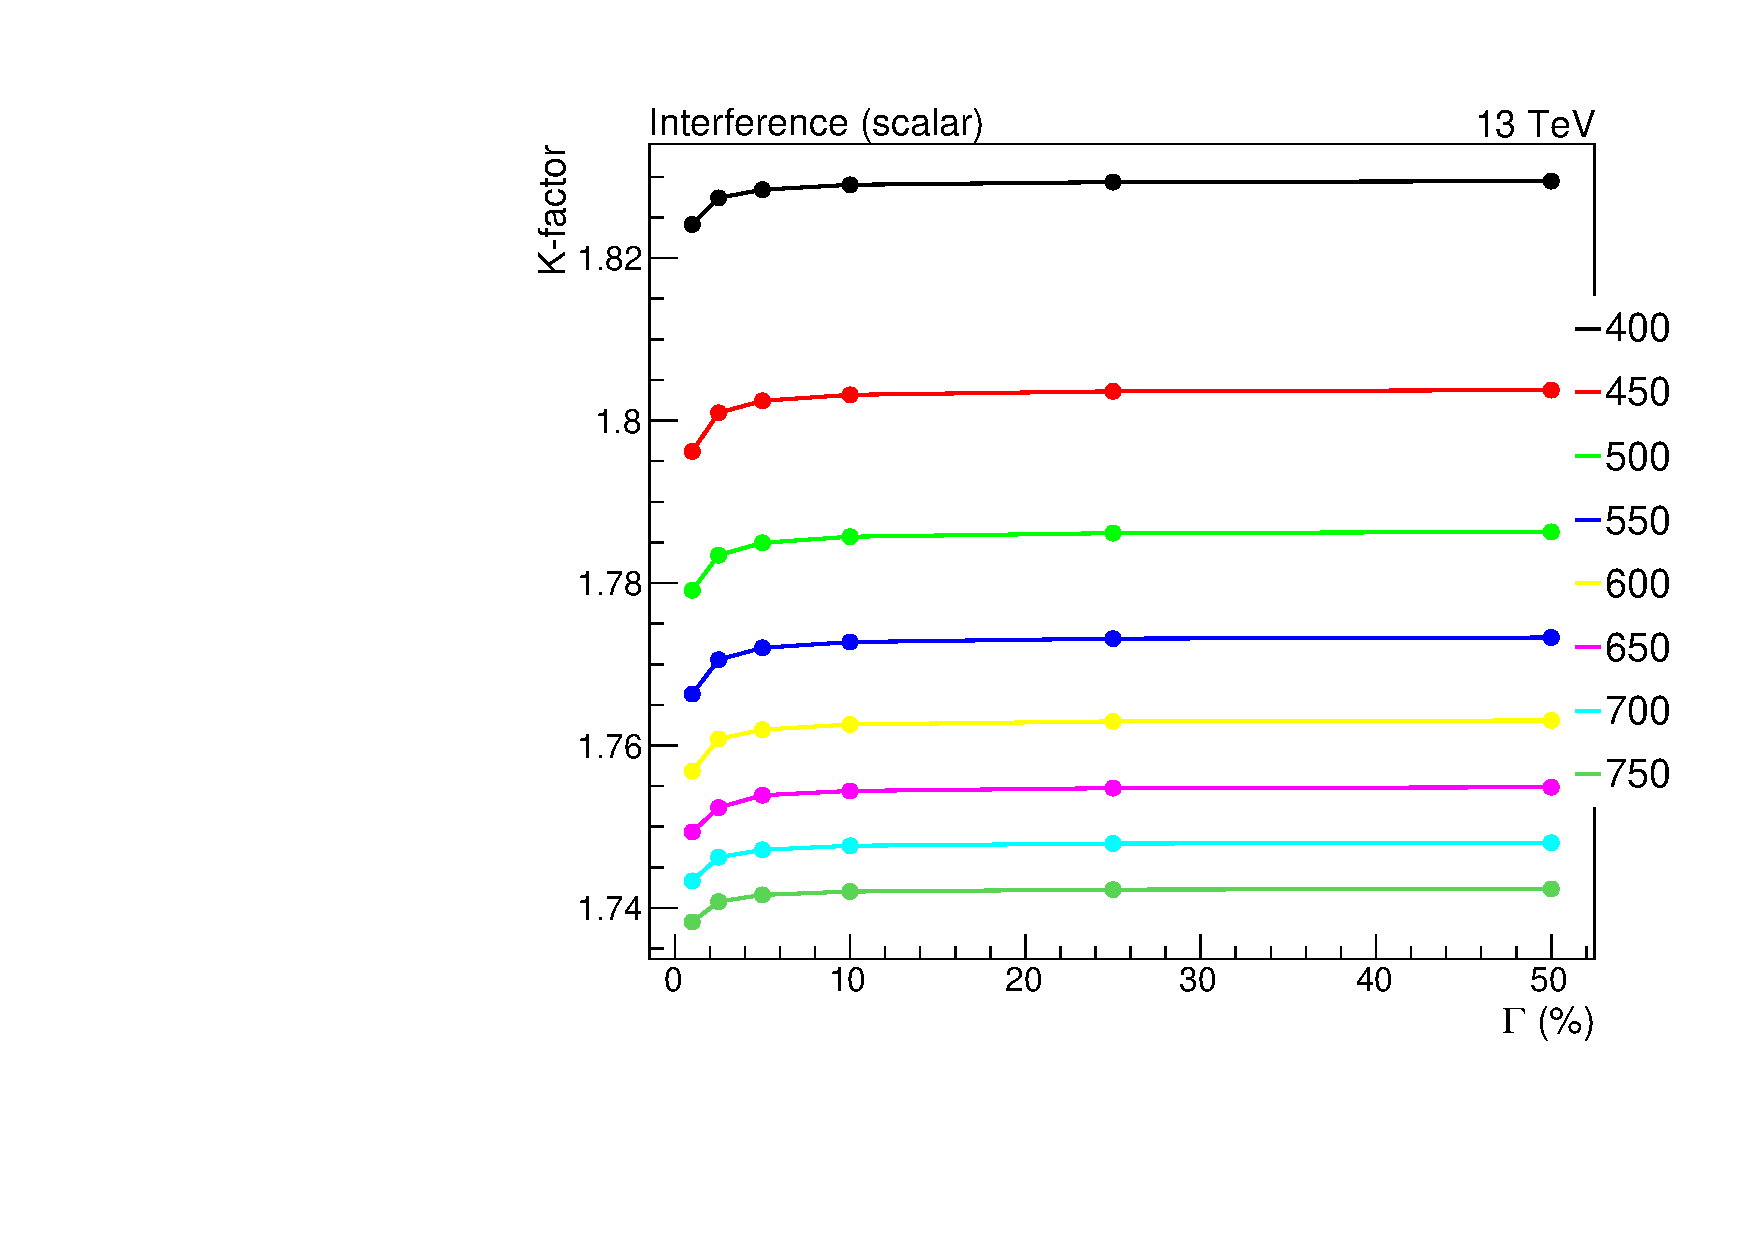
\includegraphics[width=0.45\textwidth,keepaspectratio=true]{fig/chapt8//kfactors/k_factor_Scalar_int.pdf}
\caption{Scaling factors applied to the signal-only part of the pseudoscalar signal (top left), signal-only part of the scalar signal (top right), interference part of the pseudoscalar signal (bottom left), and interference part of the scalar signal (bottom right). The factors are shown as a function of resonance width for different signal masses. Note that the y axes only show a limited range, i-e the relative variations are small.}
\label{fig:kfactors}
\end{figure}

Figure~\ref{fig:kfactors} shows a summary of the obtained scaling factors.
The scaling factors range from 2.12 for 400\,GeV signal samples to 1.71 for 750\,GeV interference samples.
The factors vary by up top 7\% as a function of mass, with the scaling factor being smaller for higher masses, and are consistent for different widths within about 1\%.

Note that we currently do not assign uncertainties in the NNLO cross sections or in the scaling factors, but we intend to add the cross section uncertainties in the next iteration.

\section{Interpolation and extrapolation to different masses and widths}
\label{sec:morphing}
In the case of the hMSSM discussed in Sec.~\ref{sec:hmssm}, it is impossible to fully cover the relevant part of the $(m_A, \tan\beta)$ spectrum with a limited set of samples in terms of fixed masses and widths, like the ones produced and discussed above.
There are a number of reasons for this:

\begin{enumerate}
        \item At low $\tan\beta$, where this search is sensitive, $m_H$ and $m_A$ are not mass-degenerate within the detector resolution. This implies that it is not possible to simply use the produced values of $m_H$ and $m_A$ and interpolate between the points scanned in this way.
        \item Furthermore, the difference between the mass points (100--150\,GeV) is larger than the mass resolution, which roughly corresponds to half this difference or worse.
        \item In addition, the width depends strongly on $\tan\beta$, which implies that, even for a given $m_A$, a quasi-continuous dependence on the width is required to be able to set consistent limits.
\end{enumerate}

This section therefore describes the algorithms with which the distributions are interpolated between different masses and widths, and in a second part how the distributions are also extrapolated to lower widths within the narrow-width approximation.

\subsection{Mass and width interpolation}

One of the input variables of the two-dimensional distributions used for the statistical evaluation is the estimated mass of the parent boson.
This reconstructed mass distribution shifts along the mass axis if the mass of the parent boson changes.
This implies that an interpolation between two parent boson masses requires a morphing of the two input mass distributions that changes (morphs) the distributions along the mass axis, and in particular that a vertical interpolation (also known as bin-by-bin morphing algorithm) cannot adequately describe intermediate masses.

It was also found that simple linear horizontal morphing algorithms do not guarantee a sufficiently good interpolation between the mass points.
Therefore, the so-called \textsc{RooMomentMorph} algorithm is used~\cite{RooMomentMorph}.
It was found that the setting \textsc{NonLinearPosFractions} gives the most consistent and overall best results.

The algorithm is applied in the following way:
\begin{itemize}
    \item As input to the algorithm, individual mass distributions in bins of the angular variable are used.
    \item These mass distributions are produced with a finer binning than the templates used for the final statistical evaluation.
    \item In each bin of the angular variable, the \textsc{RooMomentMorph} algorithm is applied, with the fine-binned distributions of all other masses (400, 500, 600, and 750\,GeV) as input.
    \item Beforehand, these fine-binned distributions are divided by the predicted cross sections (in case of the resonant contribution) or effective positive and negative contributions to the yields (in case of the interference contribution). While the morphing algorithm can technically also handle changes in normalisation, the differences in cross section between the masses are large. Dividing by these cross sections therefore improves the results and only interpolates changes in yield because of acceptance effects.
    \item The one-dimensional interpolated distributions in bins of the angular variable are then multiplied by the cross section at the target mass, stitched together to unrolled two-dimensional distributions to comply with the inputs to the statistical evaluation, and finally bins are merged to arrive at the chosen final binning.
\end{itemize}

\begin{figure}[!Hhtb]
\centering
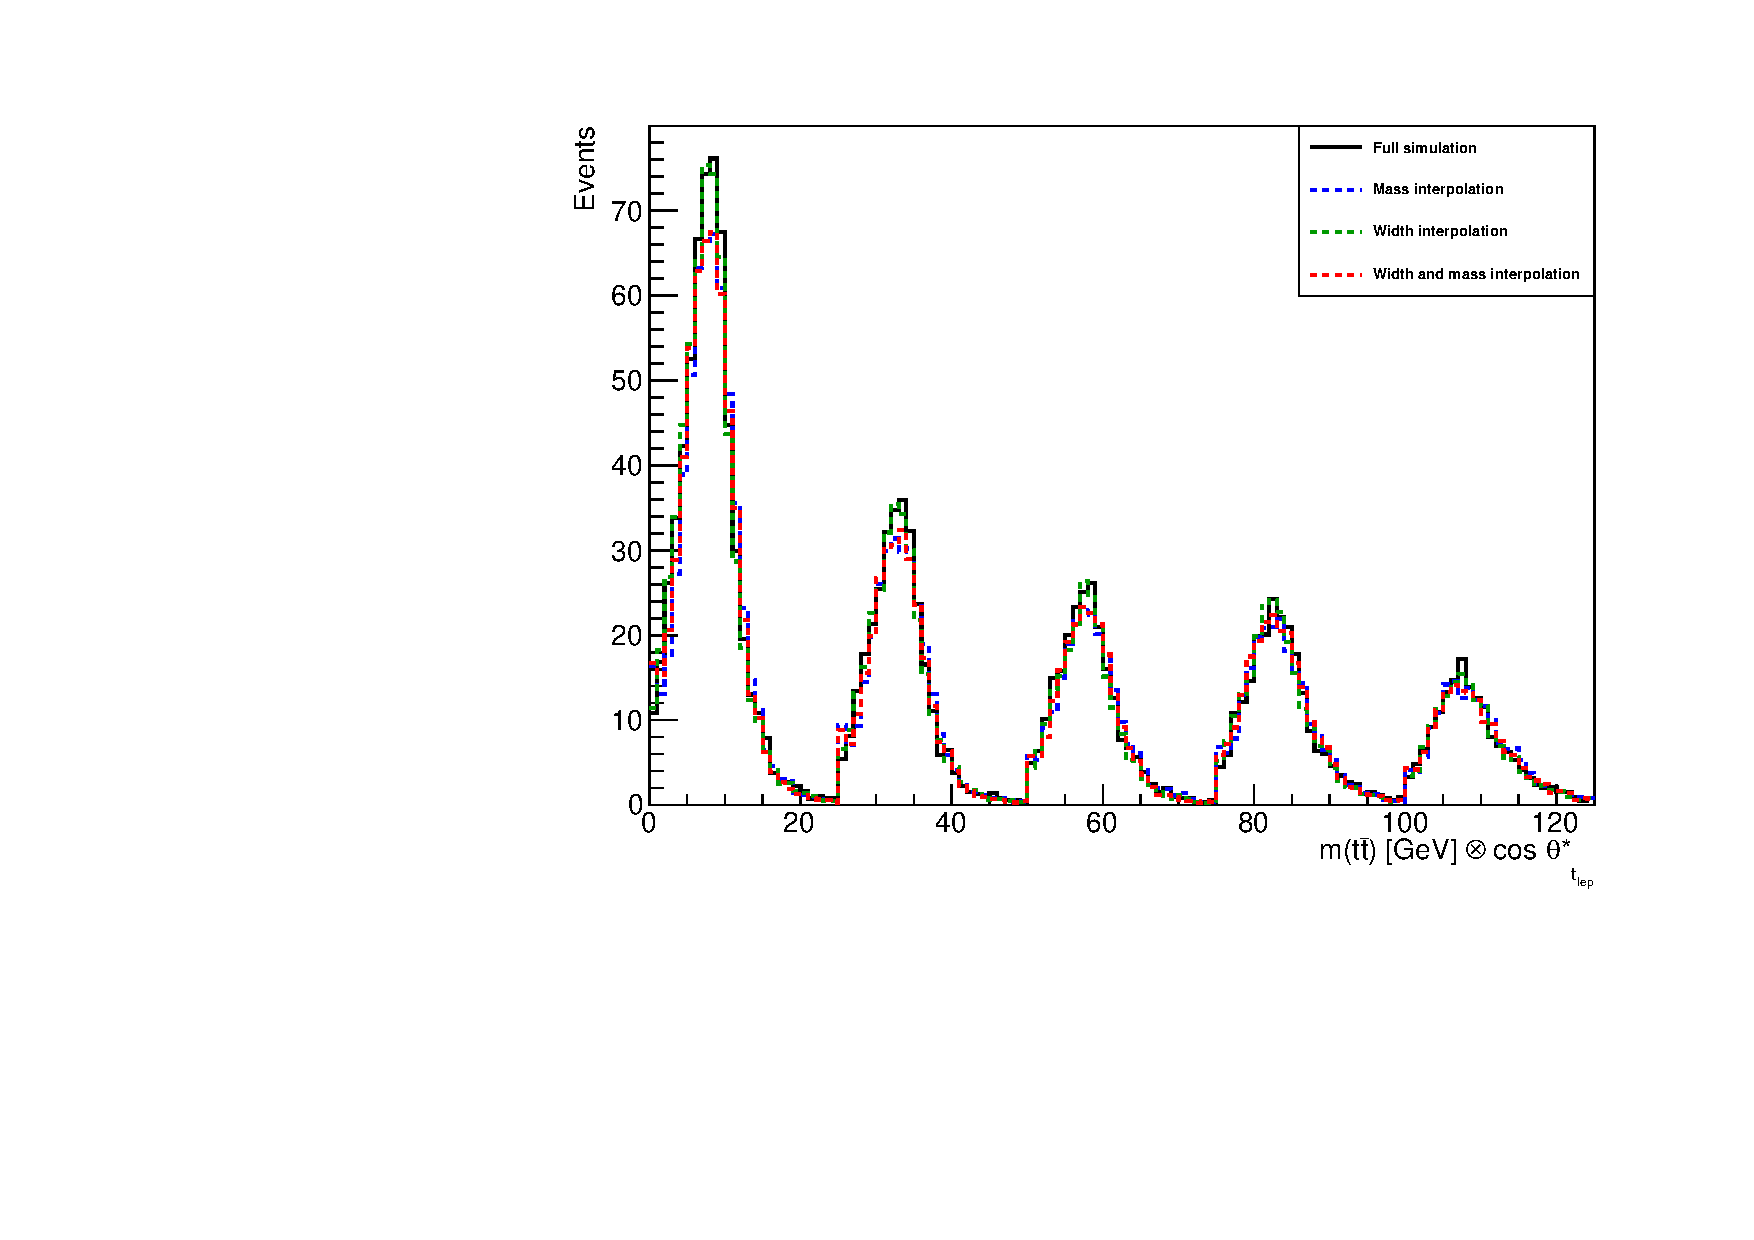
\includegraphics[width=0.7\textwidth,keepaspectratio=true]{fig/chapt8/morphing/mass_morph_mujets_pos-sgn-5pc-M500.pdf}
\caption{Comparison of unrolled m$_{t\bar t}$ distributions generated by mass morphing and width morphing with the leave-one-out strategy. The distributions are shown for the signal templates in the muon-plus-jets channel. The nominal sample at a mass of 500\,GeV and a relative width of 5\% (full simulation, red full line) is compared with the distribution obtained by interpolating between 400 and 600\,GeV (blue dashed line) and the distribution obtained by interpolating between 2.5\% and 10\% relative width (green dashed line).}
\label{fig:morph_mass_mu_sgn_500_5}
\end{figure}

\begin{figure}[!Hhtb]
\centering
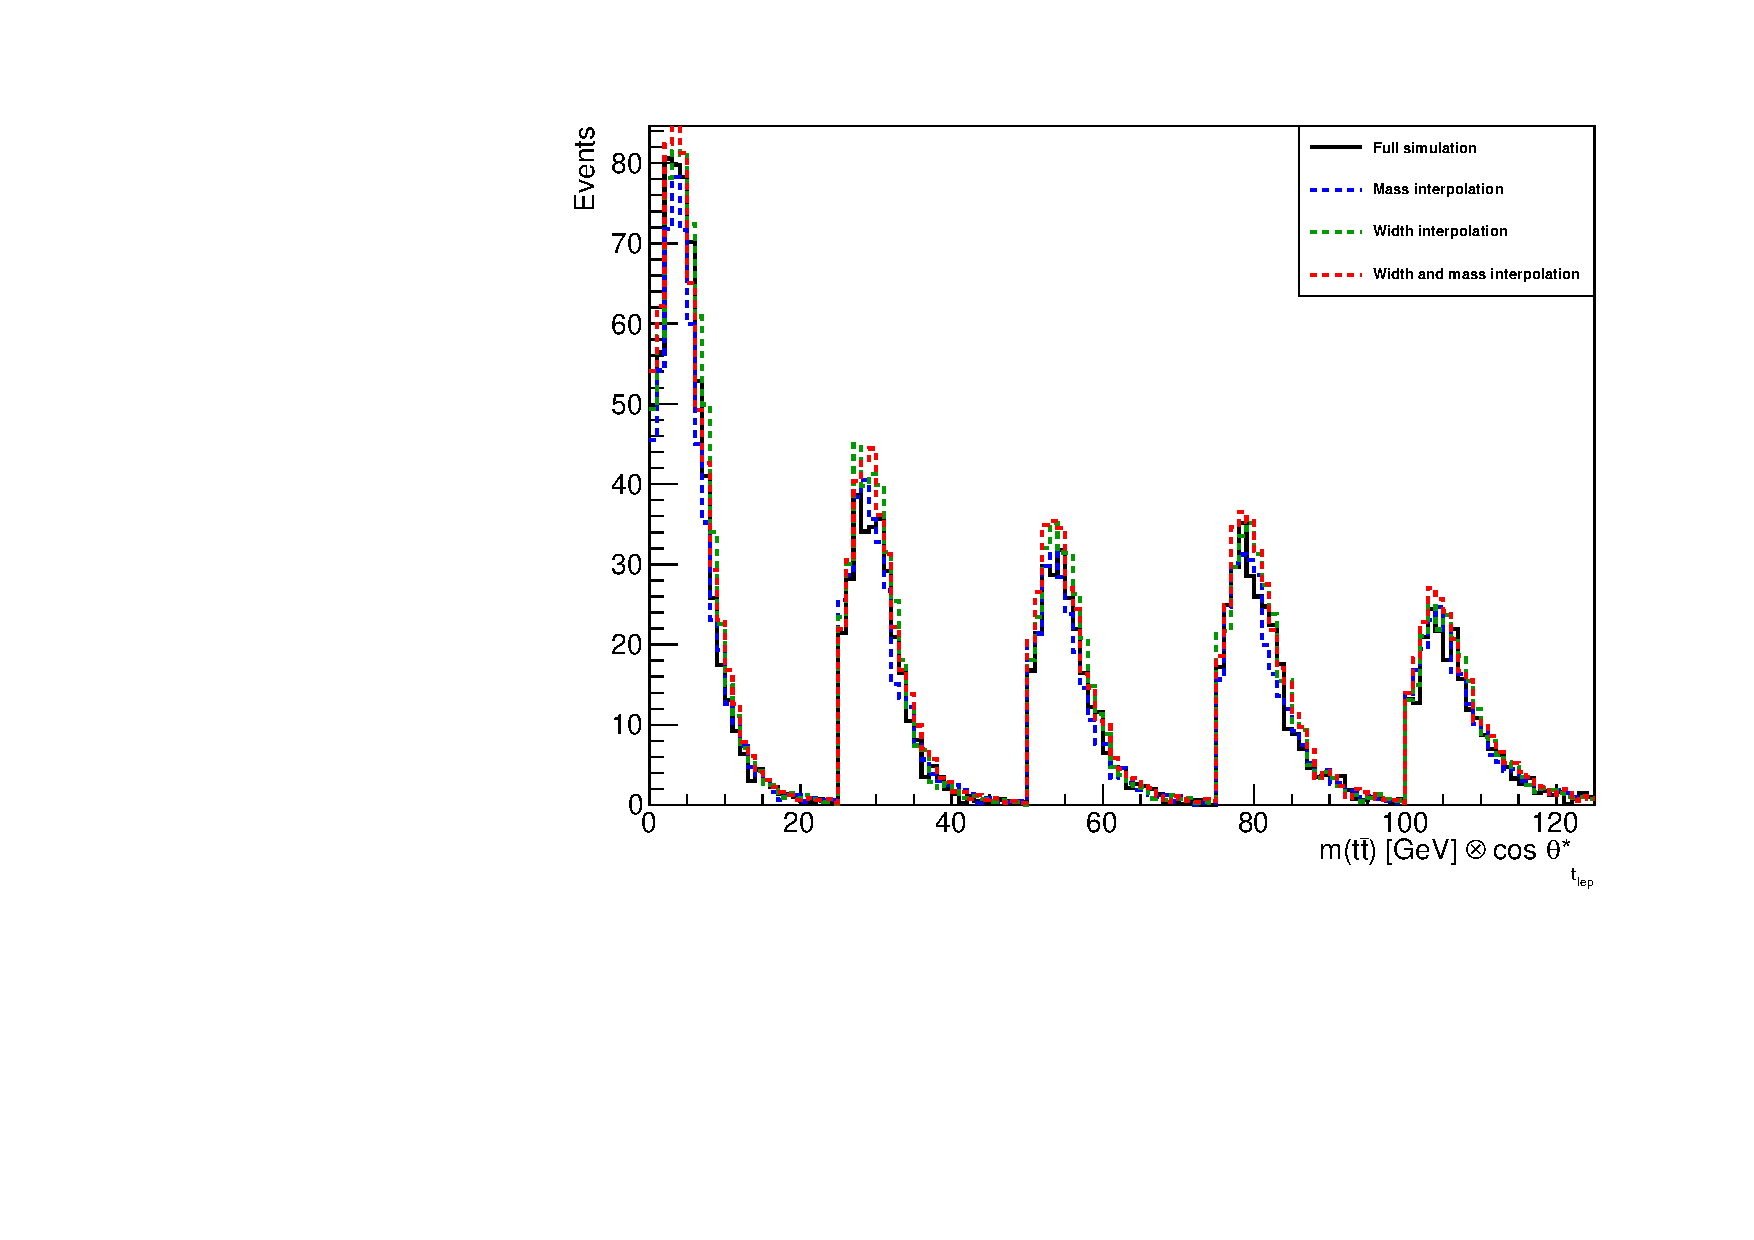
\includegraphics[width=0.7\textwidth,keepaspectratio=true]{fig/chapt8/morphing/mass_morph_mujets_pos-int-5pc-M500.pdf}
\caption{Comparison of unrolled m$_{t\bar t}$ distributions generated by mass morphing and width morphing with the leave-one-out strategy. The distributions are shown for the positive interference templates in the muon-plus-jets channel. The nominal sample at a mass of 500\,GeV and a relative width of 5\% (full simulation, red full line) is compared with the distribution obtained by interpolating between 400 and 600\,GeV (blue dashed line) and the distribution obtained by interpolating between 2.5\% and 10\% relative width (green dashed line).}
\label{fig:morph_mass_mu_posint_500_5}
\end{figure}

\begin{figure}[!Hhtb]
\centering
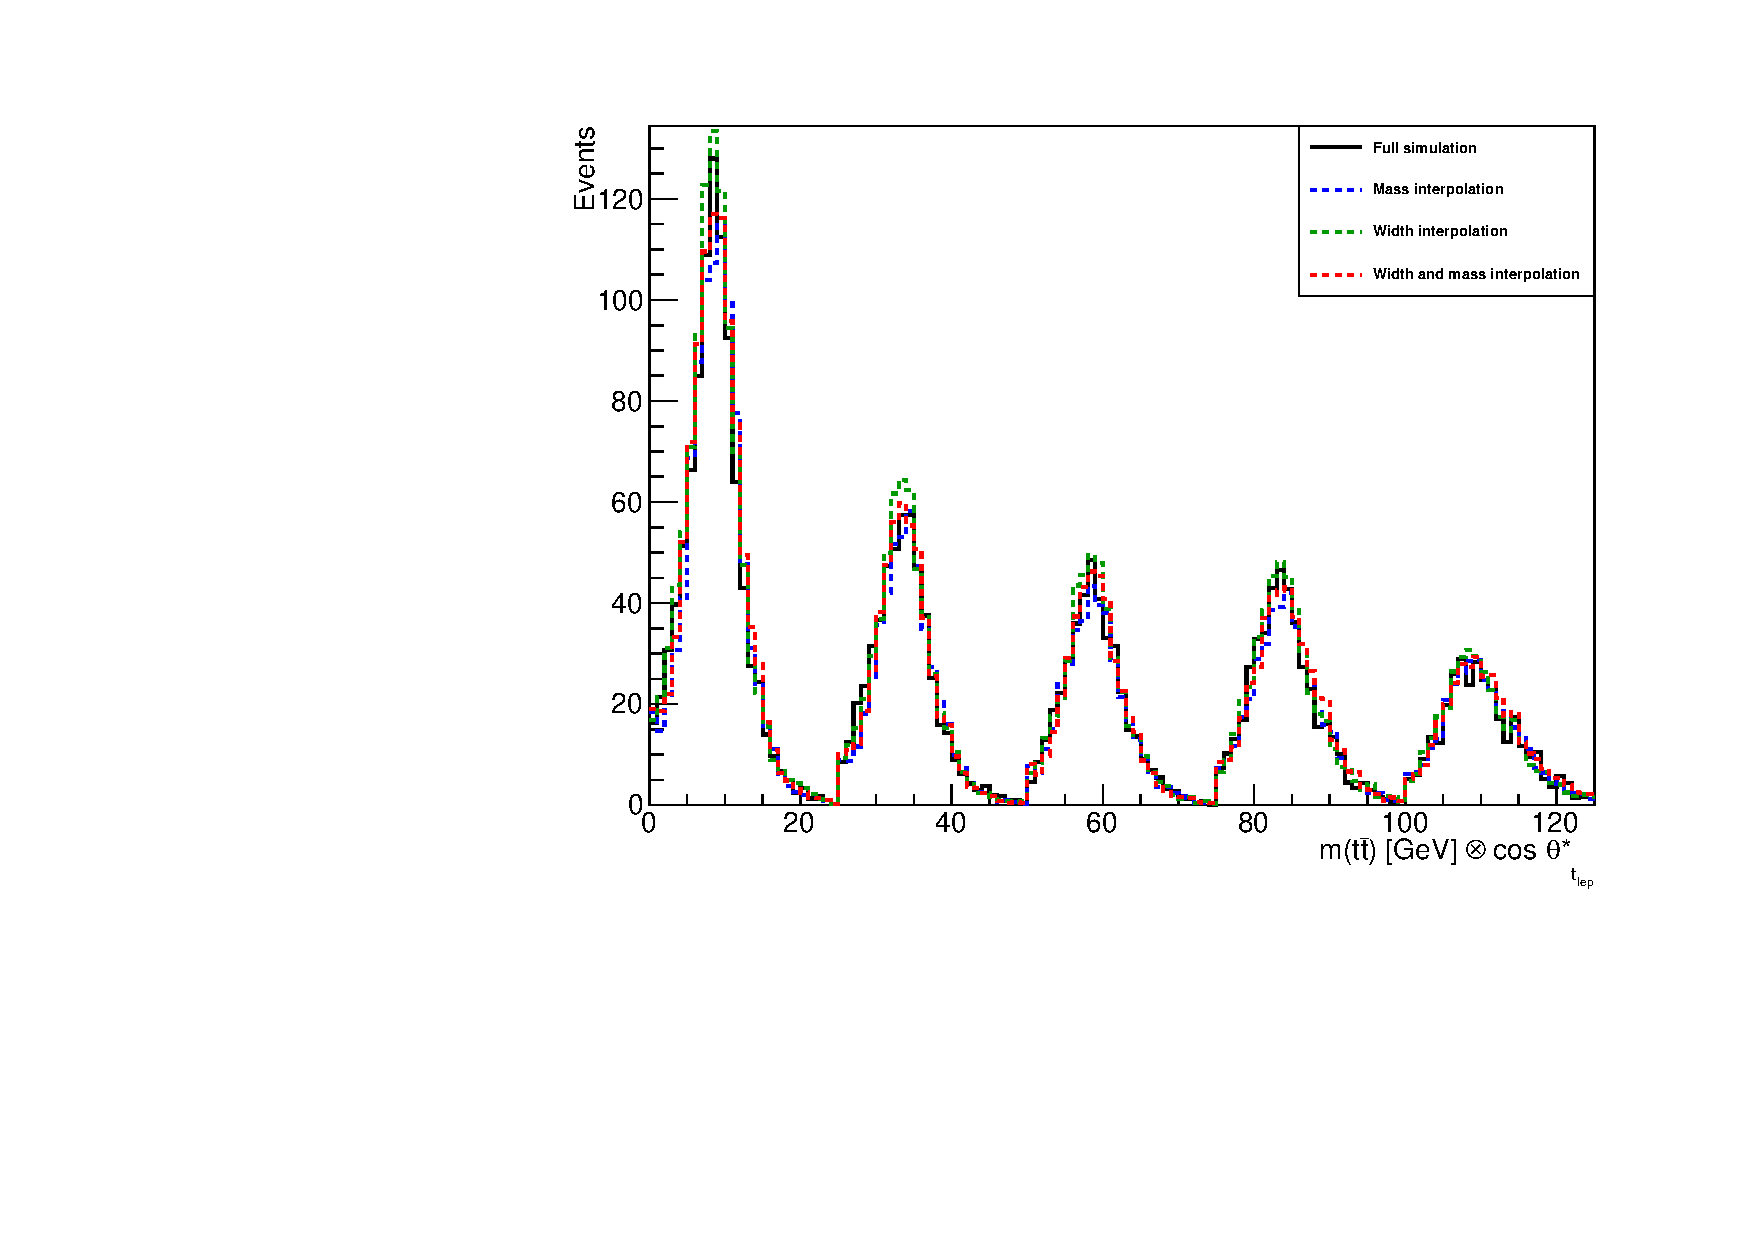
\includegraphics[width=0.7\textwidth,keepaspectratio=true]{fig/chapt8/morphing/mass_morph_mujets_neg-int-5pc-M500.pdf}
\caption{Comparison of unrolled m$_{t\bar t}$ distributions generated by mass morphing and width morphing with the leave-one-out strategy. The distributions are shown for the negative interference templates in the muon-plus-jets channel. The nominal sample at a mass of 500\,GeV and a relative width of 5\% (full simulation, red full line) is compared with the distribution obtained by interpolating between 400 and 600\,GeV (blue dashed line) and the distribution obtained by interpolating between 2.5\% and 10\% relative width (green dashed line).}
\label{fig:morph_mass_mu_negint_500_5}
\end{figure}


\begin{figure}[!Hhtb]
\centering
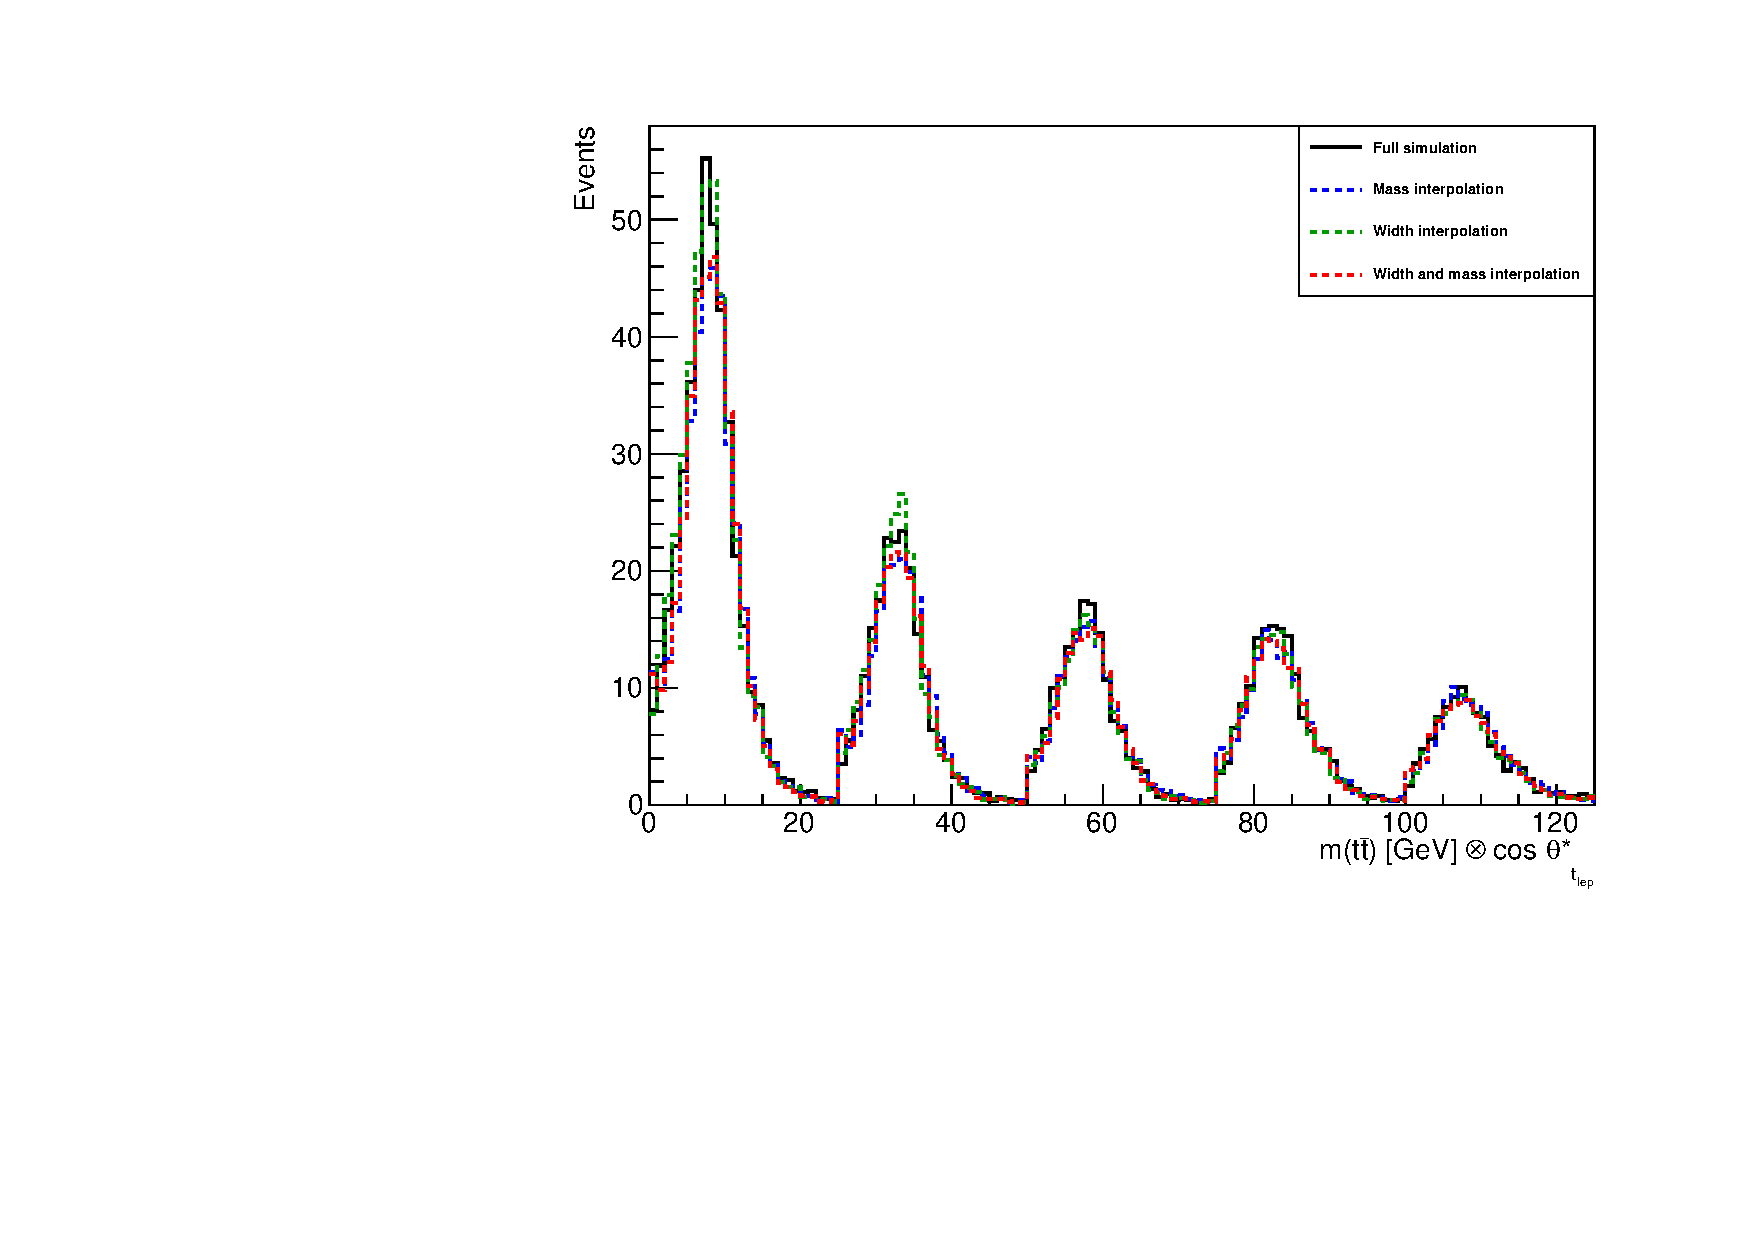
\includegraphics[width=0.7\textwidth,keepaspectratio=true]{fig/chapt8/morphing/mass_morph_ejets_pos-sgn-5pc-M500.pdf}
\caption{Comparison of unrolled  m$_{t\bar t}$distributions generated by mass morphing and width morphing with the leave-one-out strategy. The distributions are shown for the signal templates in the electron-plus-jets channel. The nominal sample at a mass of 500\,GeV and a relative width of 5\% (full simulation, red full line) is compared with the distribution obtained by interpolating between 400 and 600\,GeV (blue dashed line) and the distribution obtained by interpolating between 2.5\% and 10\% relative width (green dashed line).}
\label{fig:morph_mass_ele_sgn_500_5}
\end{figure}
\begin{figure}[!Hhtb]
\centering
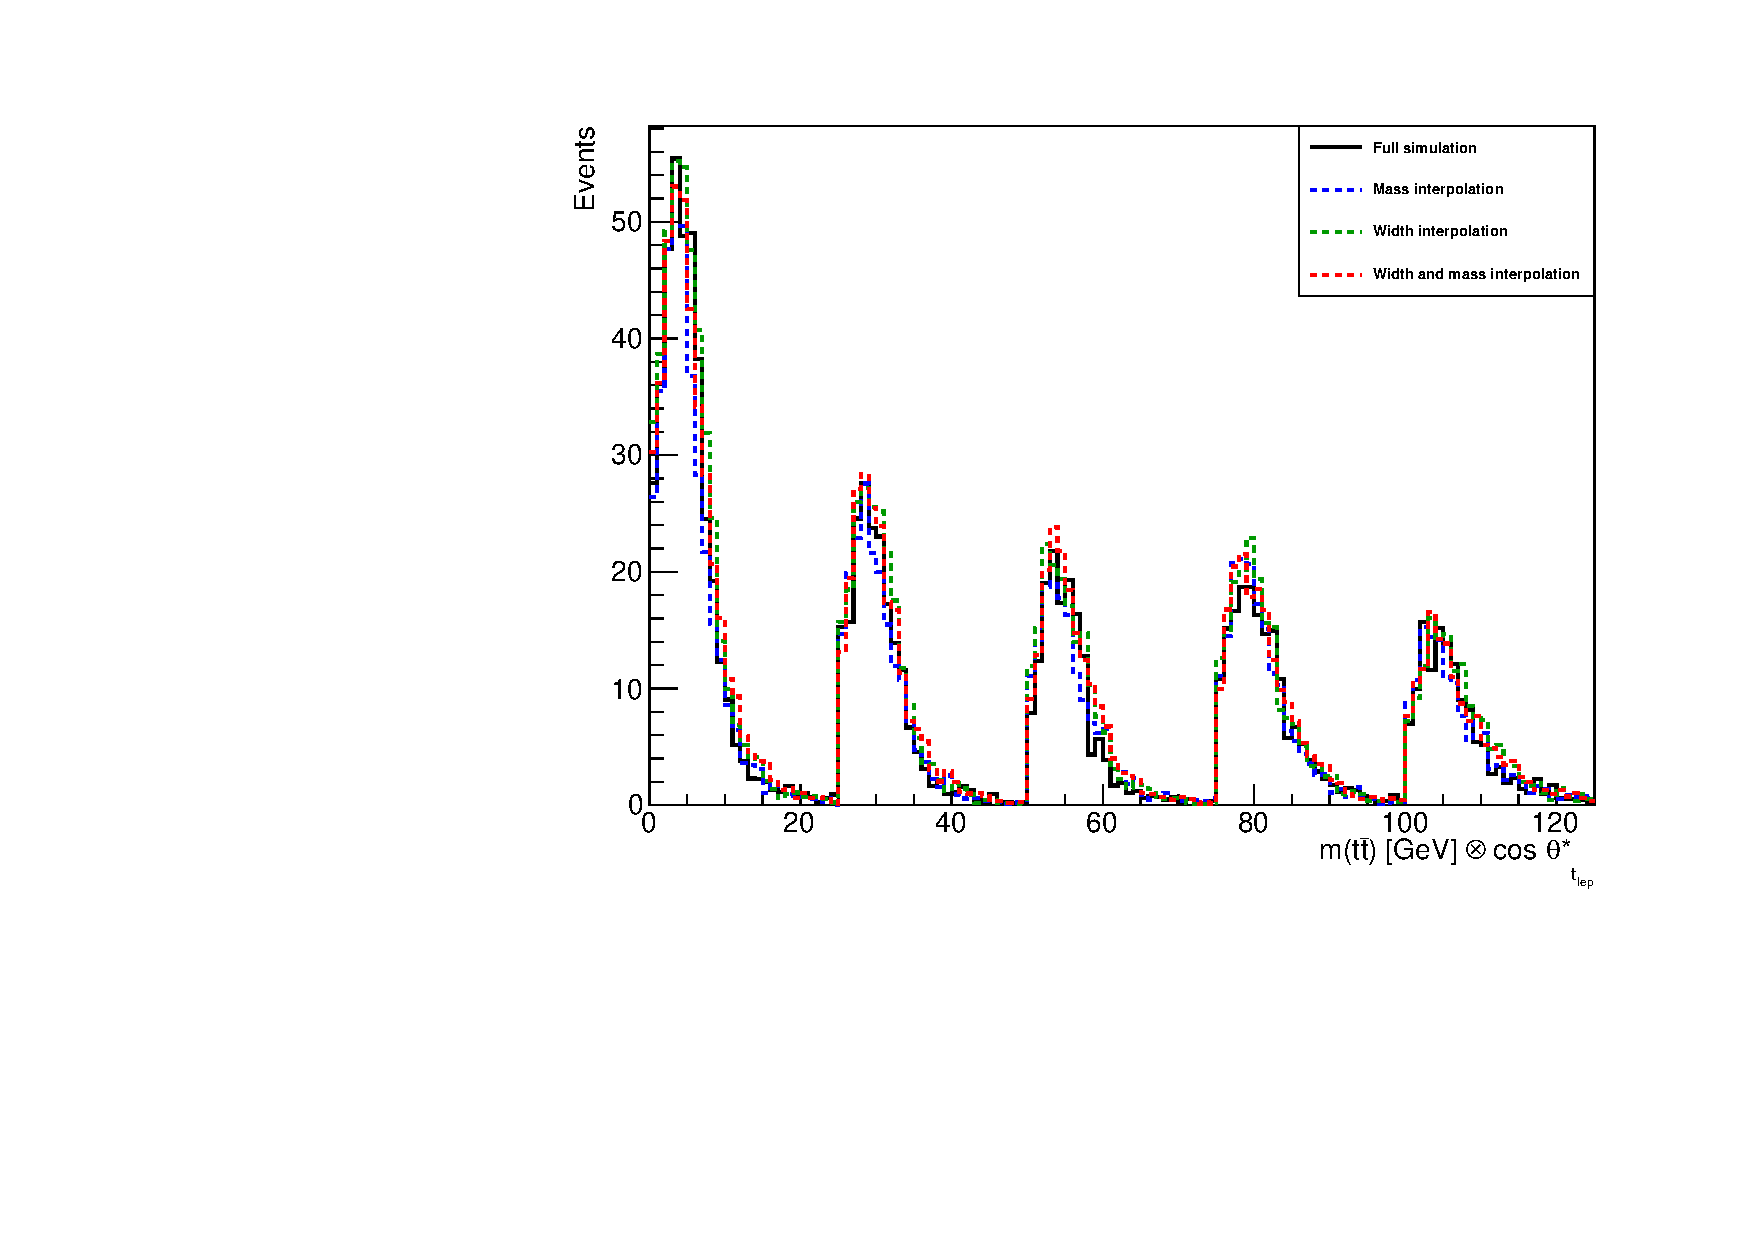
\includegraphics[width=0.7\textwidth,keepaspectratio=true]{fig/chapt8/morphing/mass_morph_ejets_pos-int-5pc-M500.pdf}
\caption{Comparison of unrolled m$_{t\bar t}$ distributions generated by mass morphing and width morphing with the leave-one-out strategy. The distributions are shown for the positive interference templates in the electron-plus-jets channel. The nominal sample at a mass of 500\,GeV and a relative width of 5\% (full simulation, red full line) is compared with the distribution obtained by interpolating between 400 and 600\,GeV (blue dashed line) and the distribution obtained by interpolating between 2.5\% and 10\% relative width (green dashed line).}
\label{fig:morph_mass_ele_posint_500_5}
\end{figure}

\begin{figure}[!Hhtb]
\centering
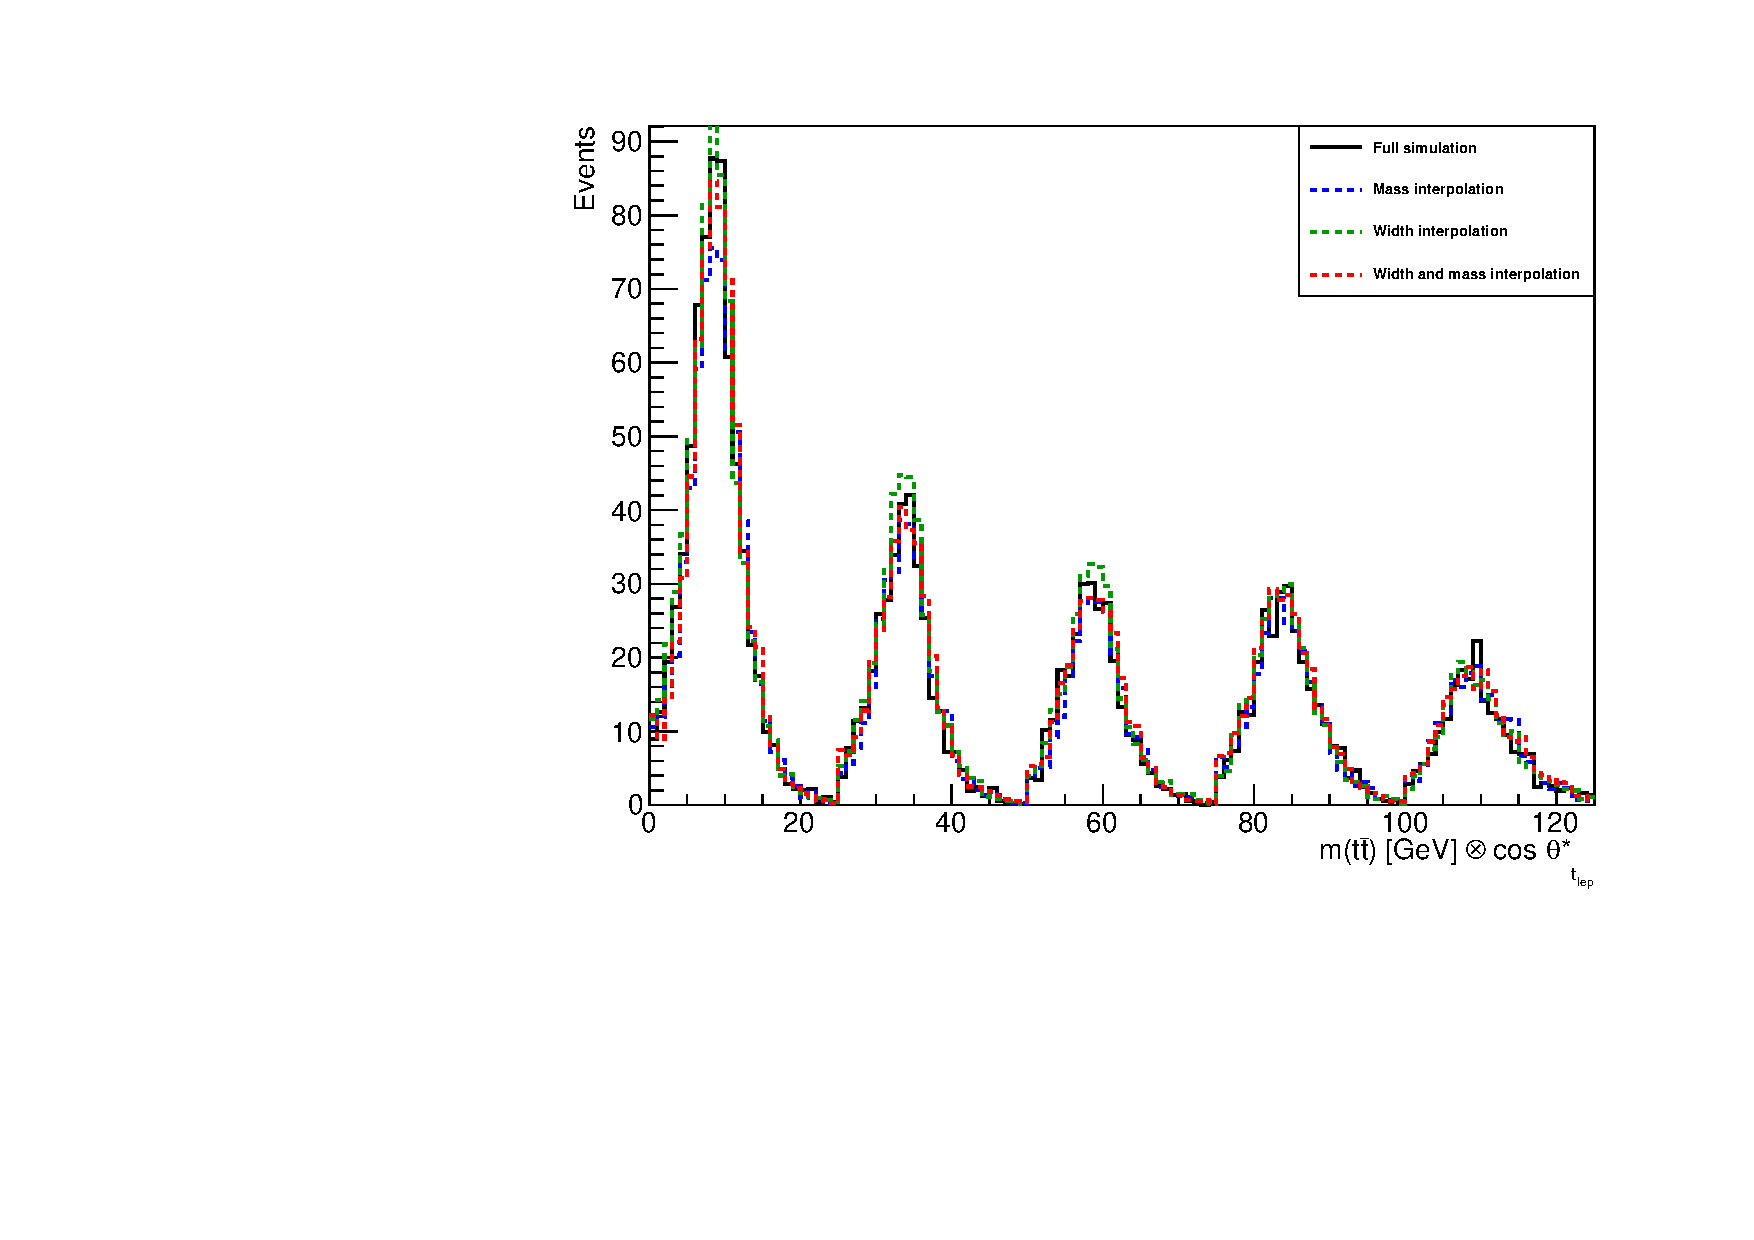
\includegraphics[width=0.7\textwidth,keepaspectratio=true]{fig/chapt8/morphing/mass_morph_ejets_neg-int-5pc-M500.pdf}
\caption{Comparison of unrolled m$_{t\bar t}$ distributions generated by mass morphing and width morphing with the leave-one-out strategy. The distributions are shown for the negative interference templates in the electron-plus-jets channel. The nominal sample at a mass of 500\,GeV and a relative width of 5\% (full simulation, red full line) is compared with the distribution obtained by interpolating between 400 and 600\,GeV (blue dashed line) and the distribution obtained by interpolating between 2.5\% and 10\% relative width (green dashed line).}
\label{fig:morph_mass_ele_negint_500_5}
\end{figure}
\begin{figure}[!Hhtb]
\centering
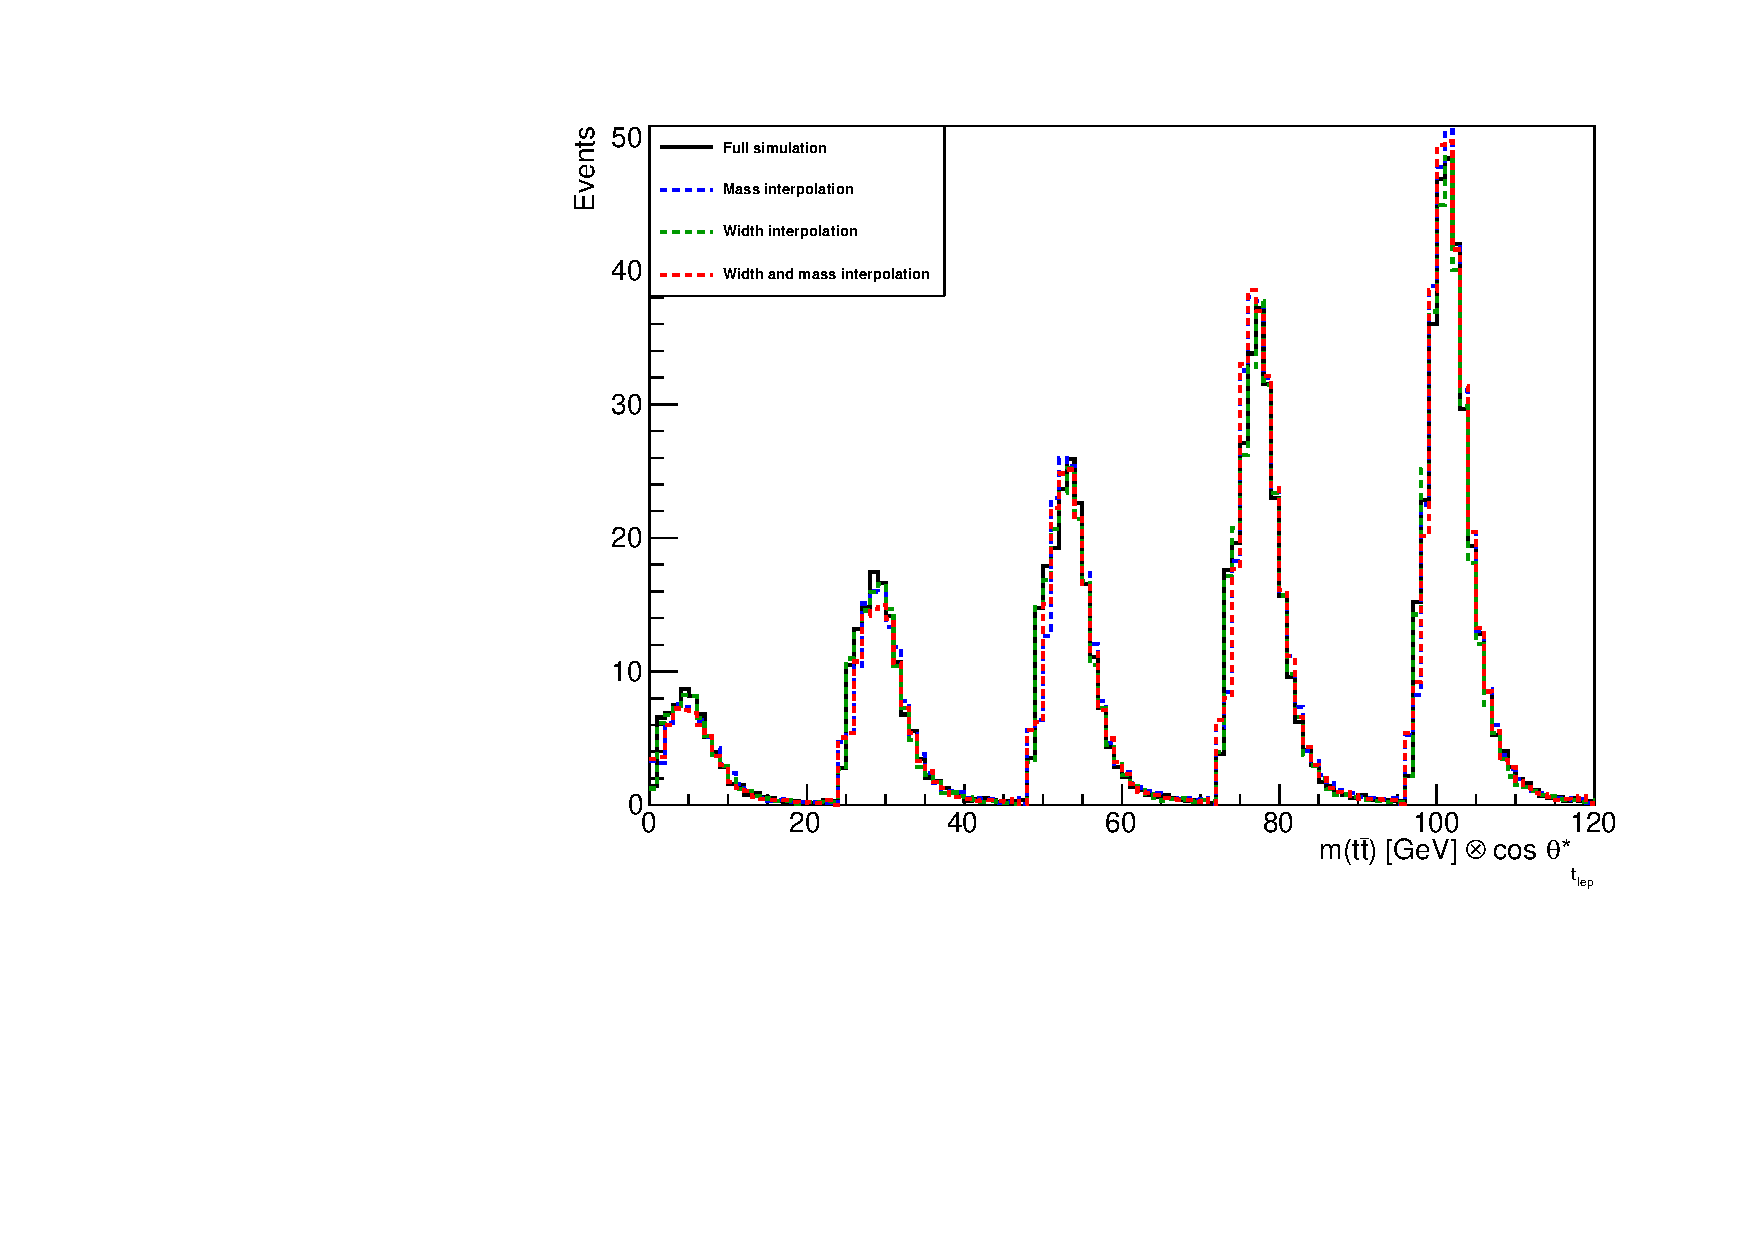
\includegraphics[width=0.7\textwidth,keepaspectratio=true]{fig/chapt8/morphing/mass_morph_ll_pos-sgn-5pc-M500.pdf}
\caption{Comparison of unrolled $m_{t\bar t}$ distributions generated by mass morphing and width morphing with the leave-one-out strategy. The distributions are shown for the signal templates in the electron-plus-jets channel. The nominal sample at a mass of 500\,GeV and a relative width of 5\% (full simulation, red full line) is compared with the distribution obtained by interpolating between 400 and 600\,GeV (blue dashed line) and the distribution obtained by interpolating between 2.5\% and 10\% relative width (green dashed line).}
\label{fig:morph_mass_ll_sgn_500_5}
\end{figure}

\begin{figure}[!Hhtb]
\centering
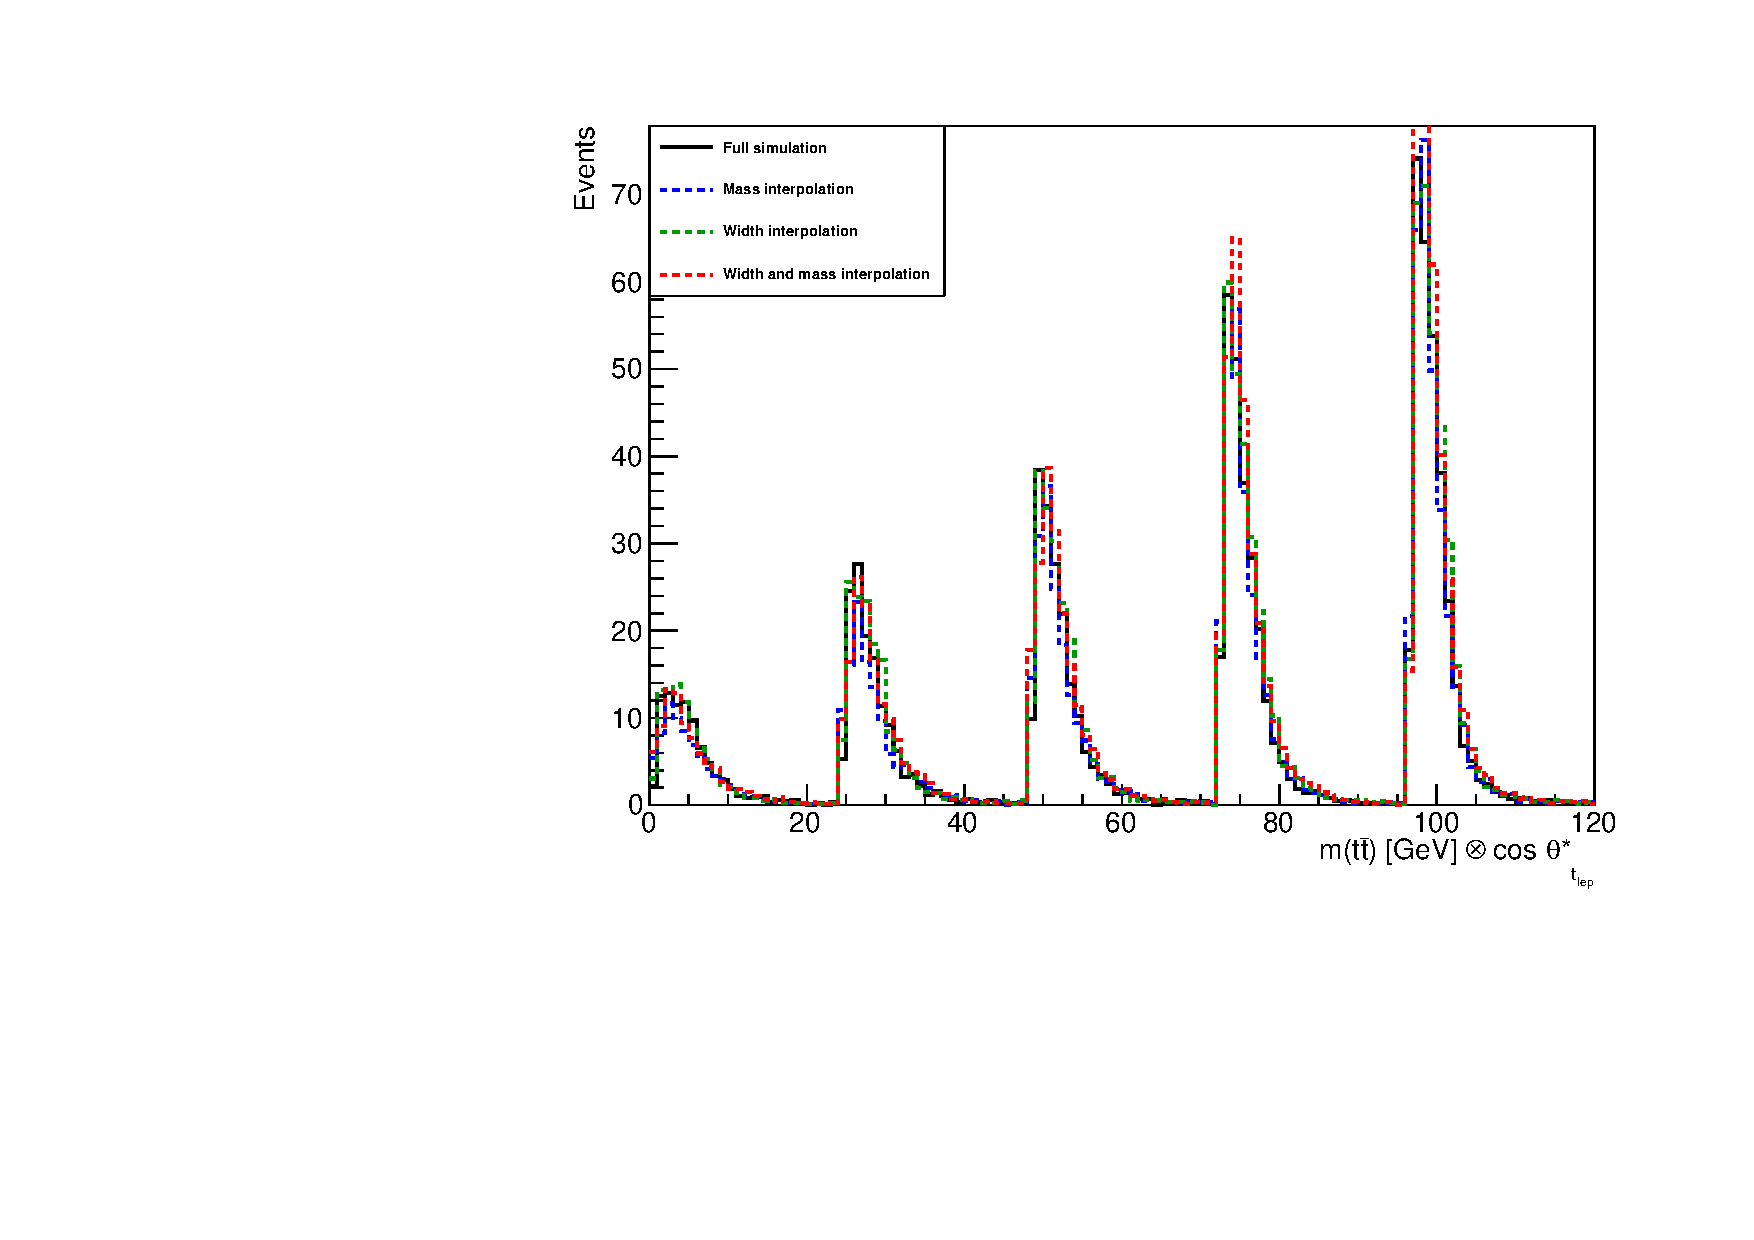
\includegraphics[width=0.7\textwidth,keepaspectratio=true]{fig/chapt8/morphing/mass_morph_ll_pos-int-5pc-M500.pdf}
\caption{Comparison of unrolled $m_{t\bar t}$ distributions generated by mass morphing and width morphing with the leave-one-out strategy. The distributions are shown for the positive interference templates in the electron-plus-jets channel. The nominal sample at a mass of 500\,GeV and a relative width of 5\% (full simulation, red full line) is compared with the distribution obtained by interpolating between 400 and 600\,GeV (blue dashed line) and the distribution obtained by interpolating between 2.5\% and 10\% relative width (green dashed line).}
\label{fig:morph_mass_ll_posint_500_5}
\end{figure}


\begin{figure}[!Hhtb]
\centering
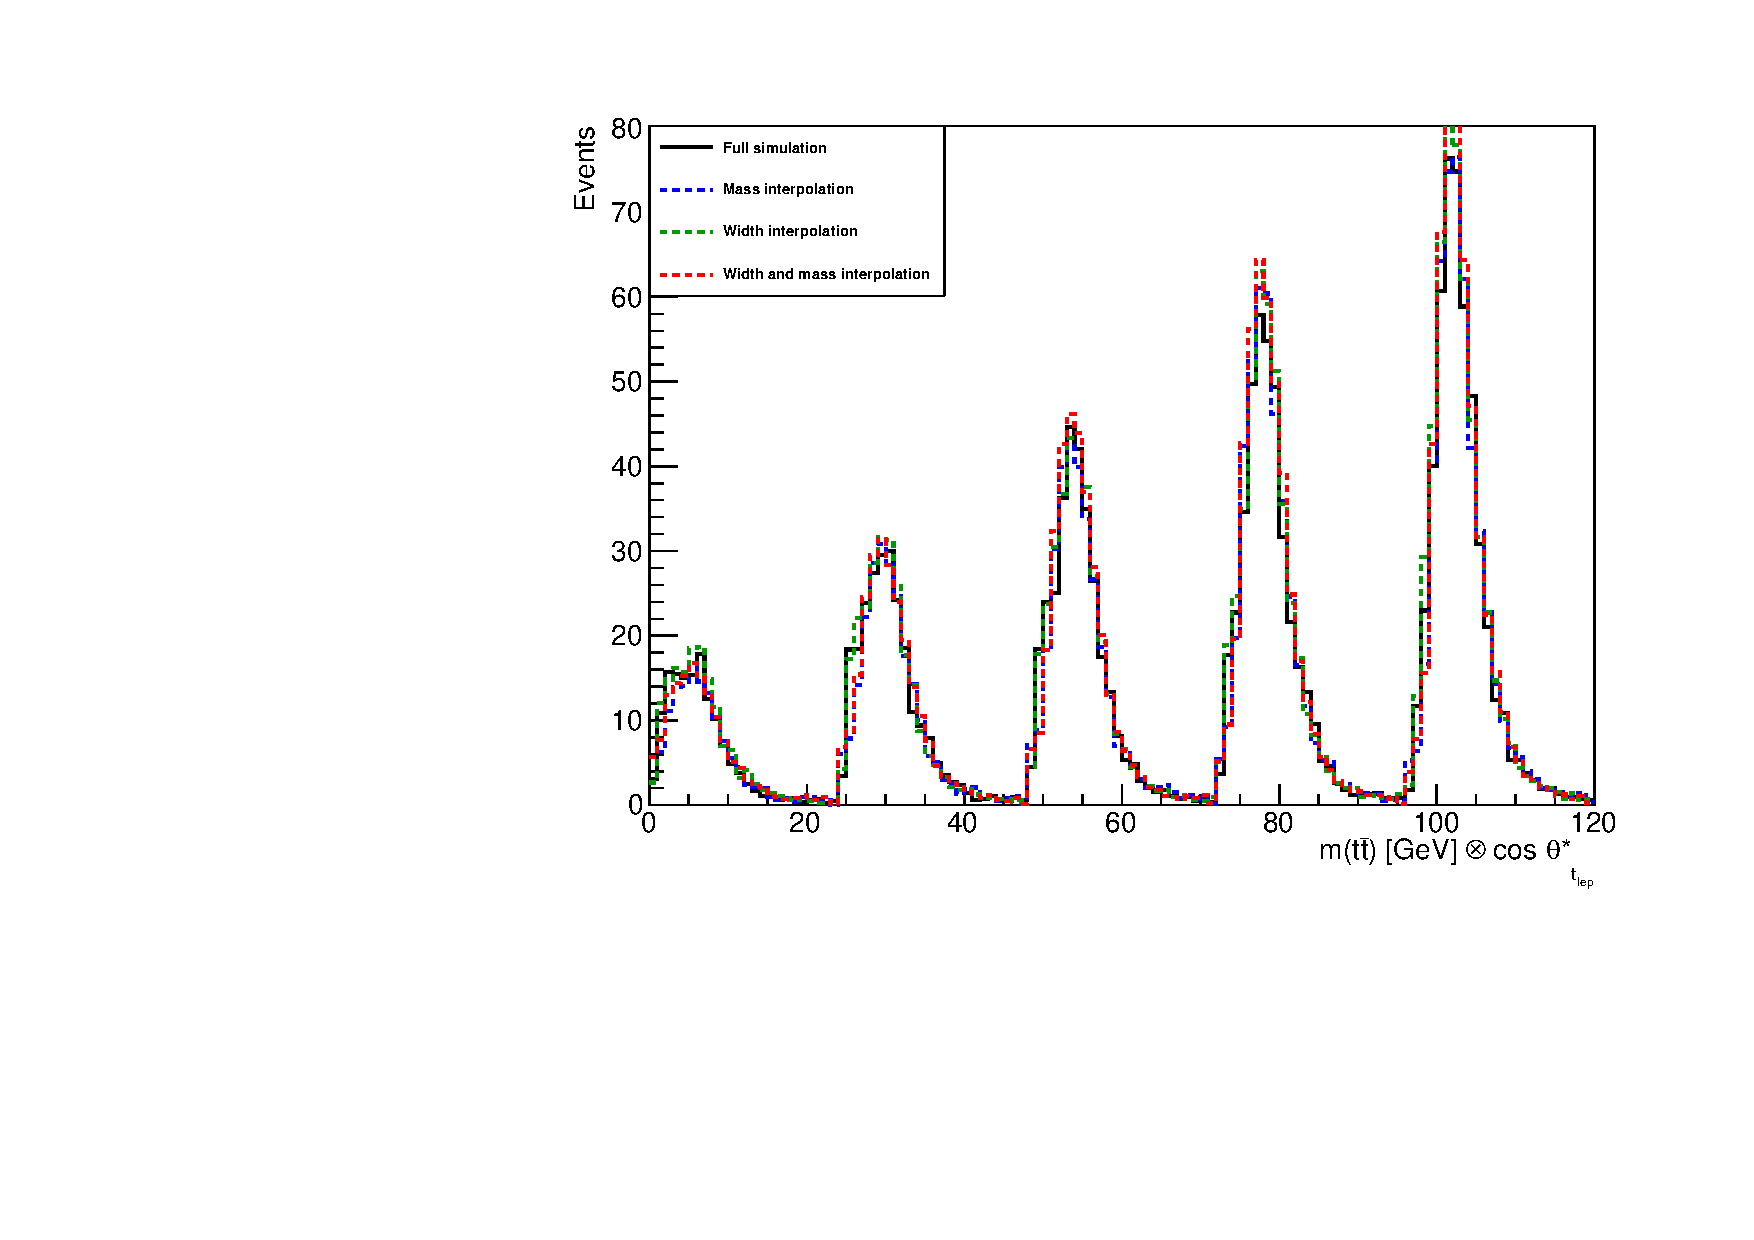
\includegraphics[width=0.7\textwidth,keepaspectratio=true]{fig/chapt8/morphing/mass_morph_ll_neg-int-5pc-M500.pdf}
\caption{Comparison of unrolled m$_{t\bar t}$ distributions generated by mass morphing and width morphing with the leave-one-out strategy. The distributions are shown for the negative interference templates in the electron-plus-jets channel. The nominal sample at a mass of 500\,GeV and a relative width of 5\% (full simulation, red full line) is compared with the distribution obtained by interpolating between 400 and 600\,GeV (blue dashed line) and the distribution obtained by interpolating between 2.5\% and 10\% relative width (green dashed line).}
\label{fig:morph_mass_ll_negint_500_5}
\end{figure}

Figures~\ref{fig:morph_mass_mu_sgn_500_5}--\ref{fig:morph_mass_ll_negint_500_5} show results of the validation performed, separately for the three different final states (muon-plus-jets, electron-plus-jets, and dilepton) and for different cases.
In this validation, the distributions of the 500\,GeV mass point are not used (``leave-one-out''), i.e.\ an interpolation between 400 and 600\,GeV (with also the 750\,GeV mass point as additional input) is performed.
In all plots, the final unrolled distributions after applying the mass interpolation algorithm are compared to the distribution obtained after full simulation.
There is overall good agreement between the interpolated and the fully simulated points.
It should be noted that the interpolation that is used for the final results only interpolates between points that are 100\,GeV apart (150\,GeV between 600 and 750\,GeV), whereas this validation is for a mass difference of 200\,GeV.

Since changing the width does generally not lead to a shift in horizontal distribution but rather to a shift only of the width of the distribution, a bin-wise interpolation can be performed in this case.
The cross section for the resonant part scales with 1/width.
Therefore, a hyperbolic interpolation is performed in this case.
The yield of the interference part only exhibits a mild dependence on the resonance width.
In this case, a linear extrapolation is performed.

Figures~\ref{fig:morph_mass_mu_sgn_500_5}--\ref{fig:morph_mass_ll_negint_500_5} also show results of the validation of the width interpolation.
The validation is also performed with the ``leave-one-out'' strategy.
Here, the points with 5\% relative width are obtained by interpolating between the distributions with 2.5\% and 10\% relative width, and compared again to the fully simulated points with 5\% relative width.
Similar to the mass morphing, a good agreement is observed between the nominal templates and the ones obtained by the interpolation.


\subsection{Width extrapolation}

The analysis is sensitive to widths below the lowest produced relative width, which has a value of 2.5\%.
However, with the mass resolution being of order of 10--15\% in the lepton-plus-jets-channel, and worse in the dilepton channel, it is expected that the signal lineshapes for widths with values of less than 2.5\% are well reproduced by the lineshapes at 2.5\% width.
We validate this narrow-width approximation in the following using the samples with 2.5\% and 5.0\% relative width.

\begin{figure}[!Hhtb]
\centering
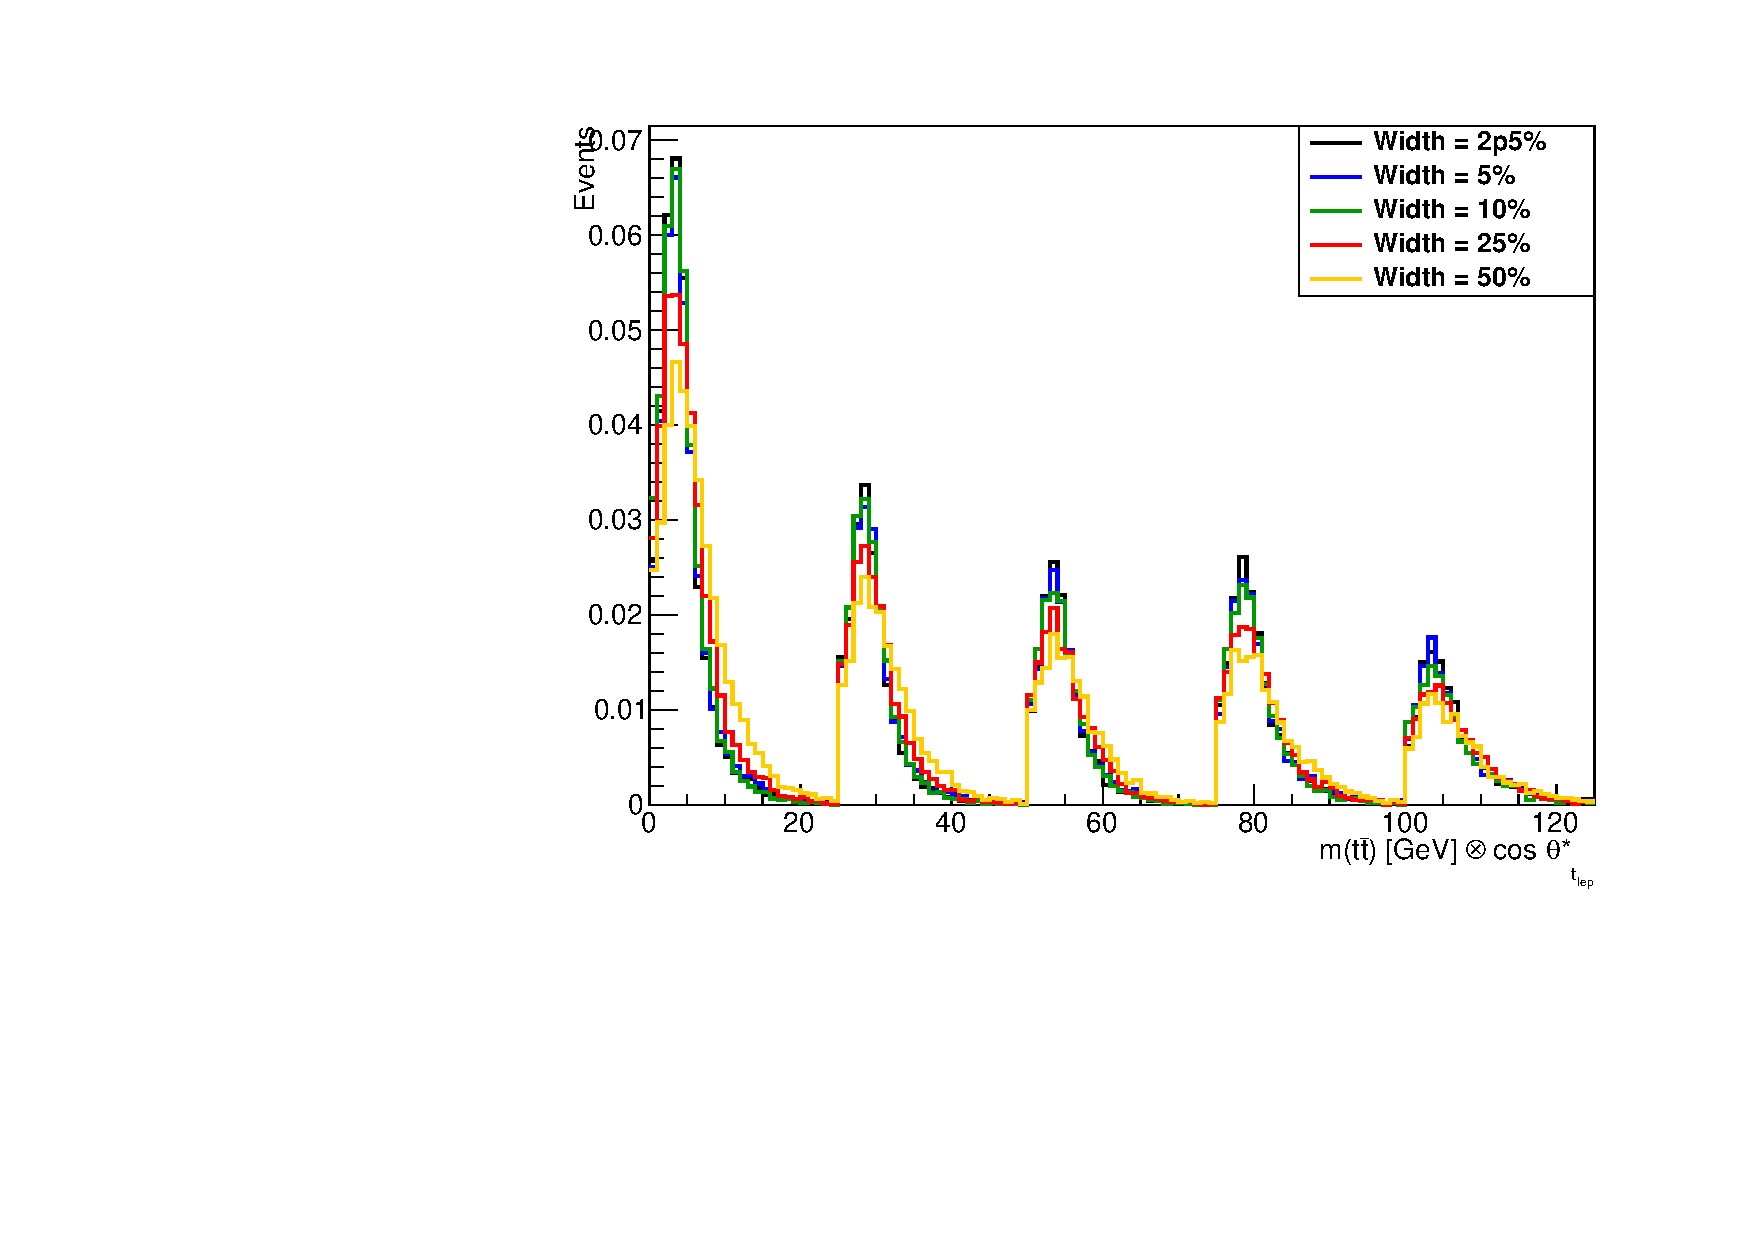
\includegraphics[width=0.7\textwidth,keepaspectratio=true]{fig/chapt8/narrow/narrow_width_mujets_pos-sgn-M400.pdf}
\caption{Comparison of unrolled m$_{t\bar t}$ distributions for different widths in the muon-plus-jets-channel and for a mass of 400\,GeV, for the resonant signal contribution.}
\label{fig:narrow_signal}
\end{figure}

\begin{figure}[!Hhtb]
\centering
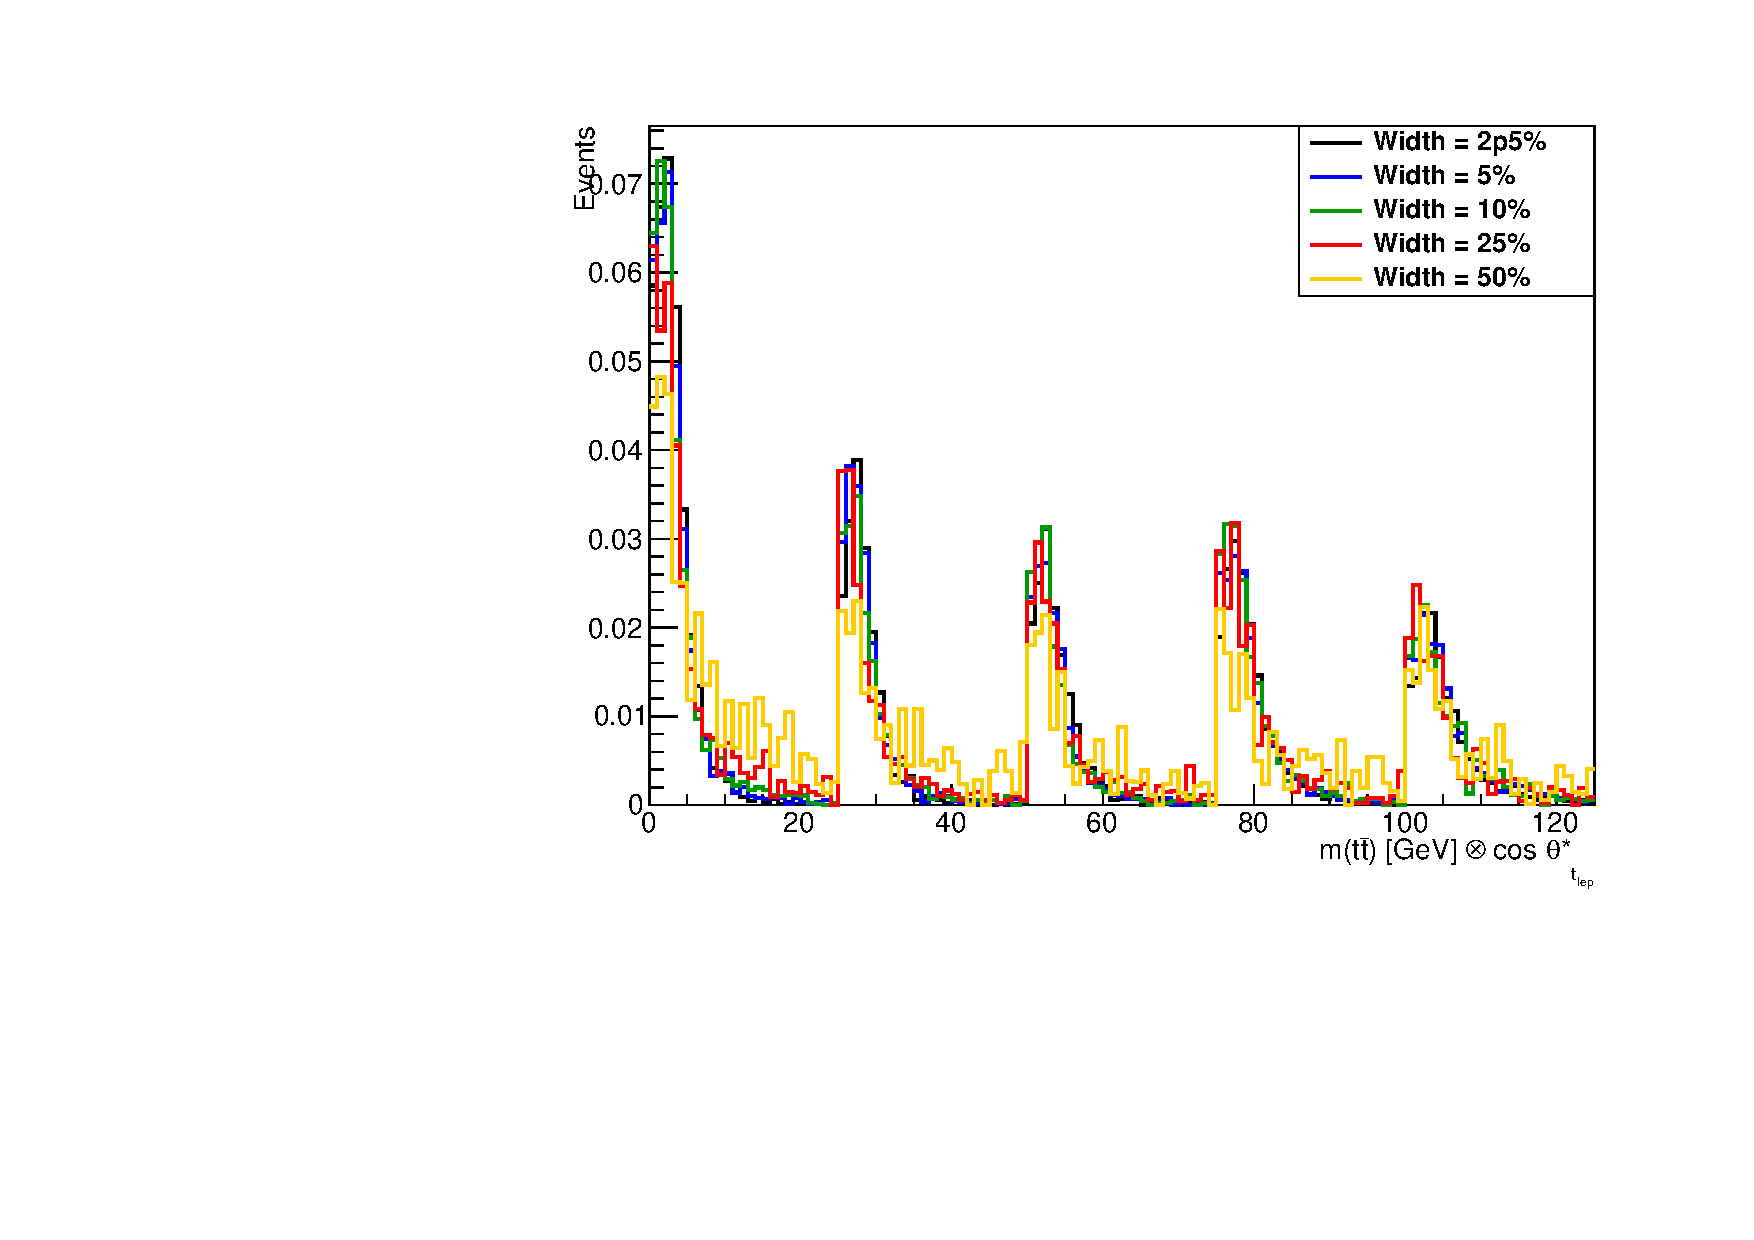
\includegraphics[width=0.7\textwidth,keepaspectratio=true]{fig/chapt8/narrow/narrow_width_mujets_pos-int-M400.pdf}
\caption{Comparison of unrolled m$_{t\bar t}$ distributions for different widths in the muon-plus-jets-channel and for a mass of 400\,GeV, for the positive interference contribution.}
\label{fig:narrow_posint}
\end{figure}


\begin{figure}[!Hhtb]
\centering
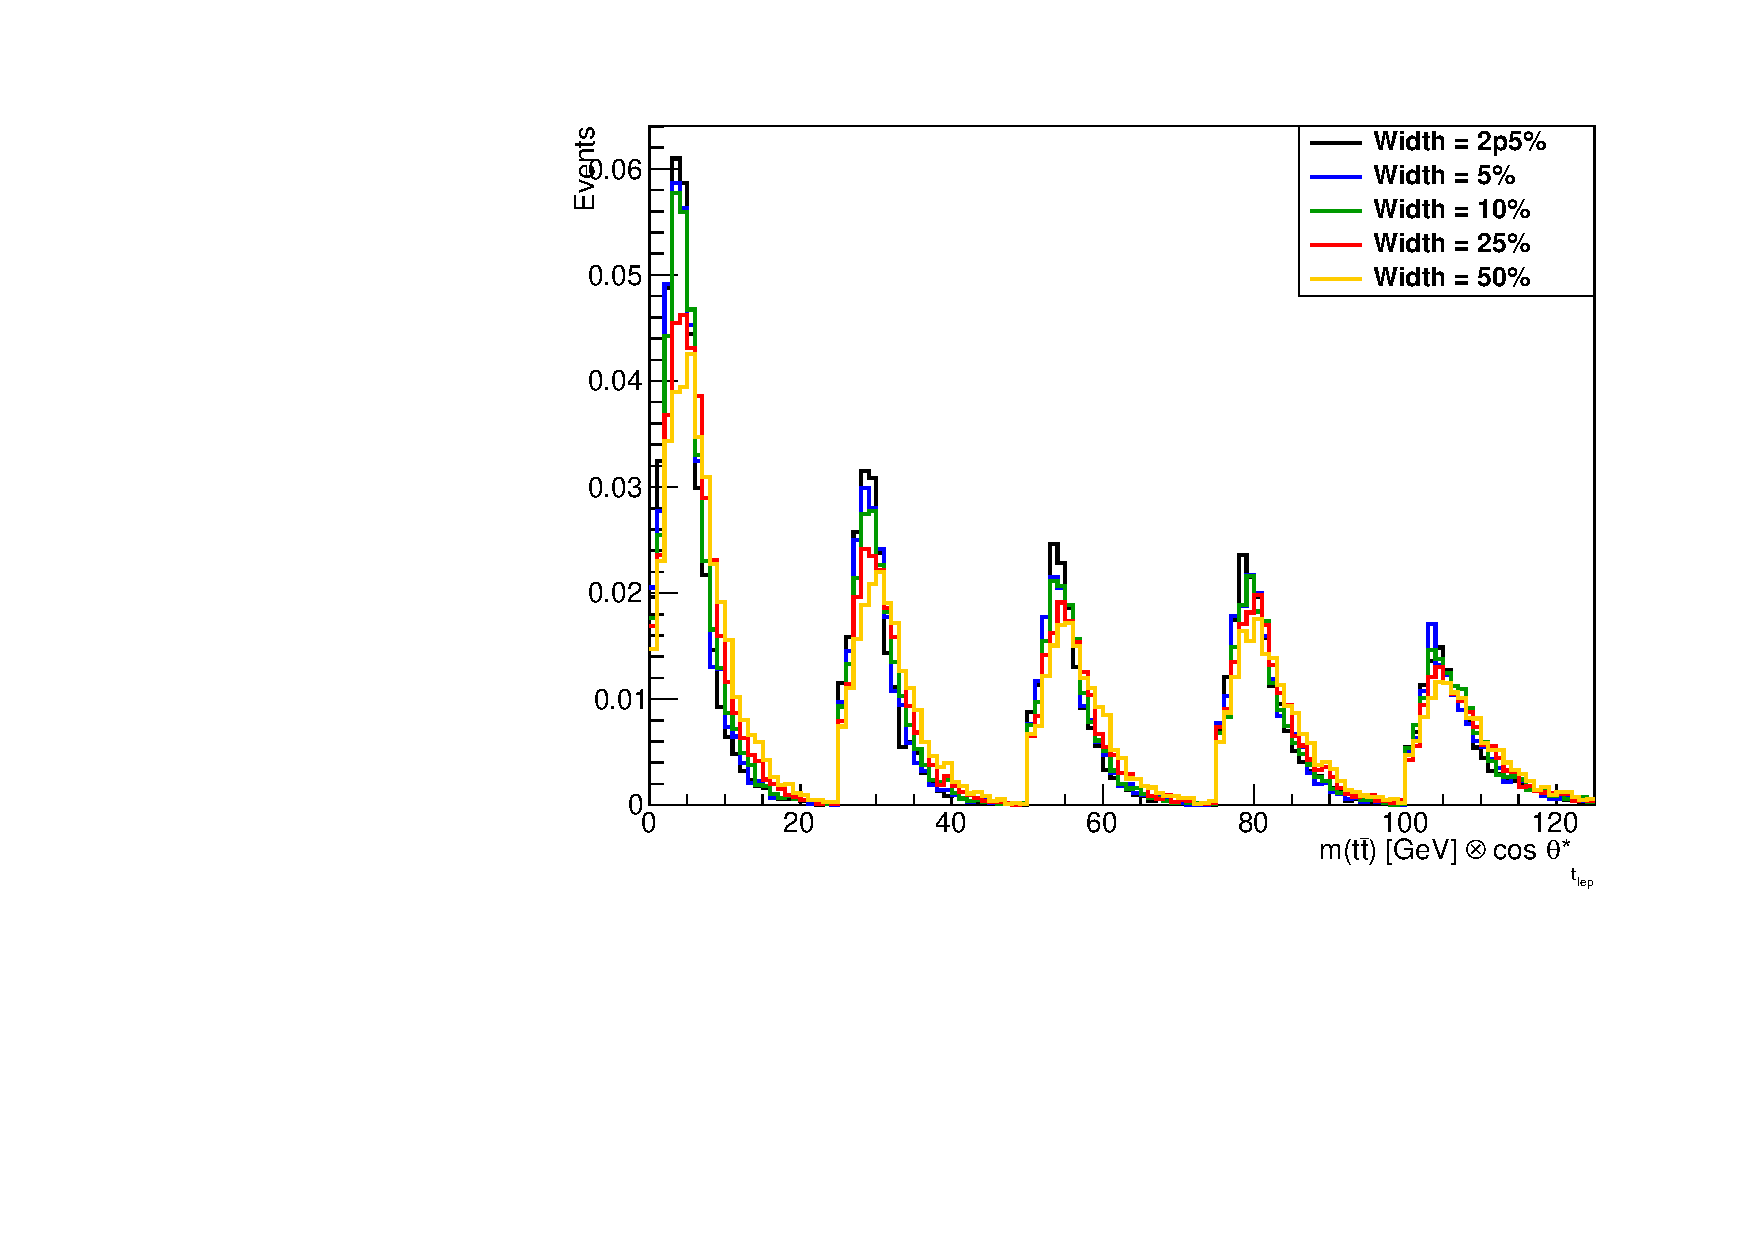
\includegraphics[width=0.7\textwidth,keepaspectratio=true]{fig/chapt8/narrow/narrow_width_mujets_neg-int-M400.pdf}
\caption{Comparison of unrolled m$_{t\bar t}$ distributions for different widths in the muon-plus-jets-channel and for a mass of 400\,GeV, for the negative interference contribution.}
\label{fig:narrow_negint}
\end{figure}

Figures~\ref{fig:narrow_signal}--\ref{fig:narrow_negint} illustrate this by comparing the lineshapes for the different signal contributions (resonant, positive interference, and negative interference) for different relative widths.
The distributions for 2.5\% and 5\% relative width are very similar, whereas there are sizeable differences between the templates for larger widths.

To conclude, we construct additional templates at widths of 0.1 and 1\%, and at intermediate widths if needed, by taking the lineshapes at 2.5\% width and scaling the expected yield by the ratio of the expected cross sections (or expected yields for the interference) at the narrower width and at 2.5\% width.

\section{Results}
\label{sec:results}
The results in the following are obtained with the CL$_\text{S}$ criterion, using the usual LHC test statistic and using the asymptotic approximation.
The asymptotic approximation has been verified for single mass and width points by comparing to the limits obtained with the full CL$_\text{S}$ method based on pseudoexperiments.

\subsection{Model-independent limits}

Model-independent upper limits on the coupling strength modifier are presented.
The upper limits are derived as a function of width and mass.
The results are given in two representations, either as function of mass in bins of relative width, or vice versa.
The upper limits on the coupling modifier are derived separately for the scalar and pseudoscalar signal models.
All results in this section are for the combination of all final states.
No scaling of the cross sections to higher orders is applied.

\begin{figure}[!Hhtb]
\centering
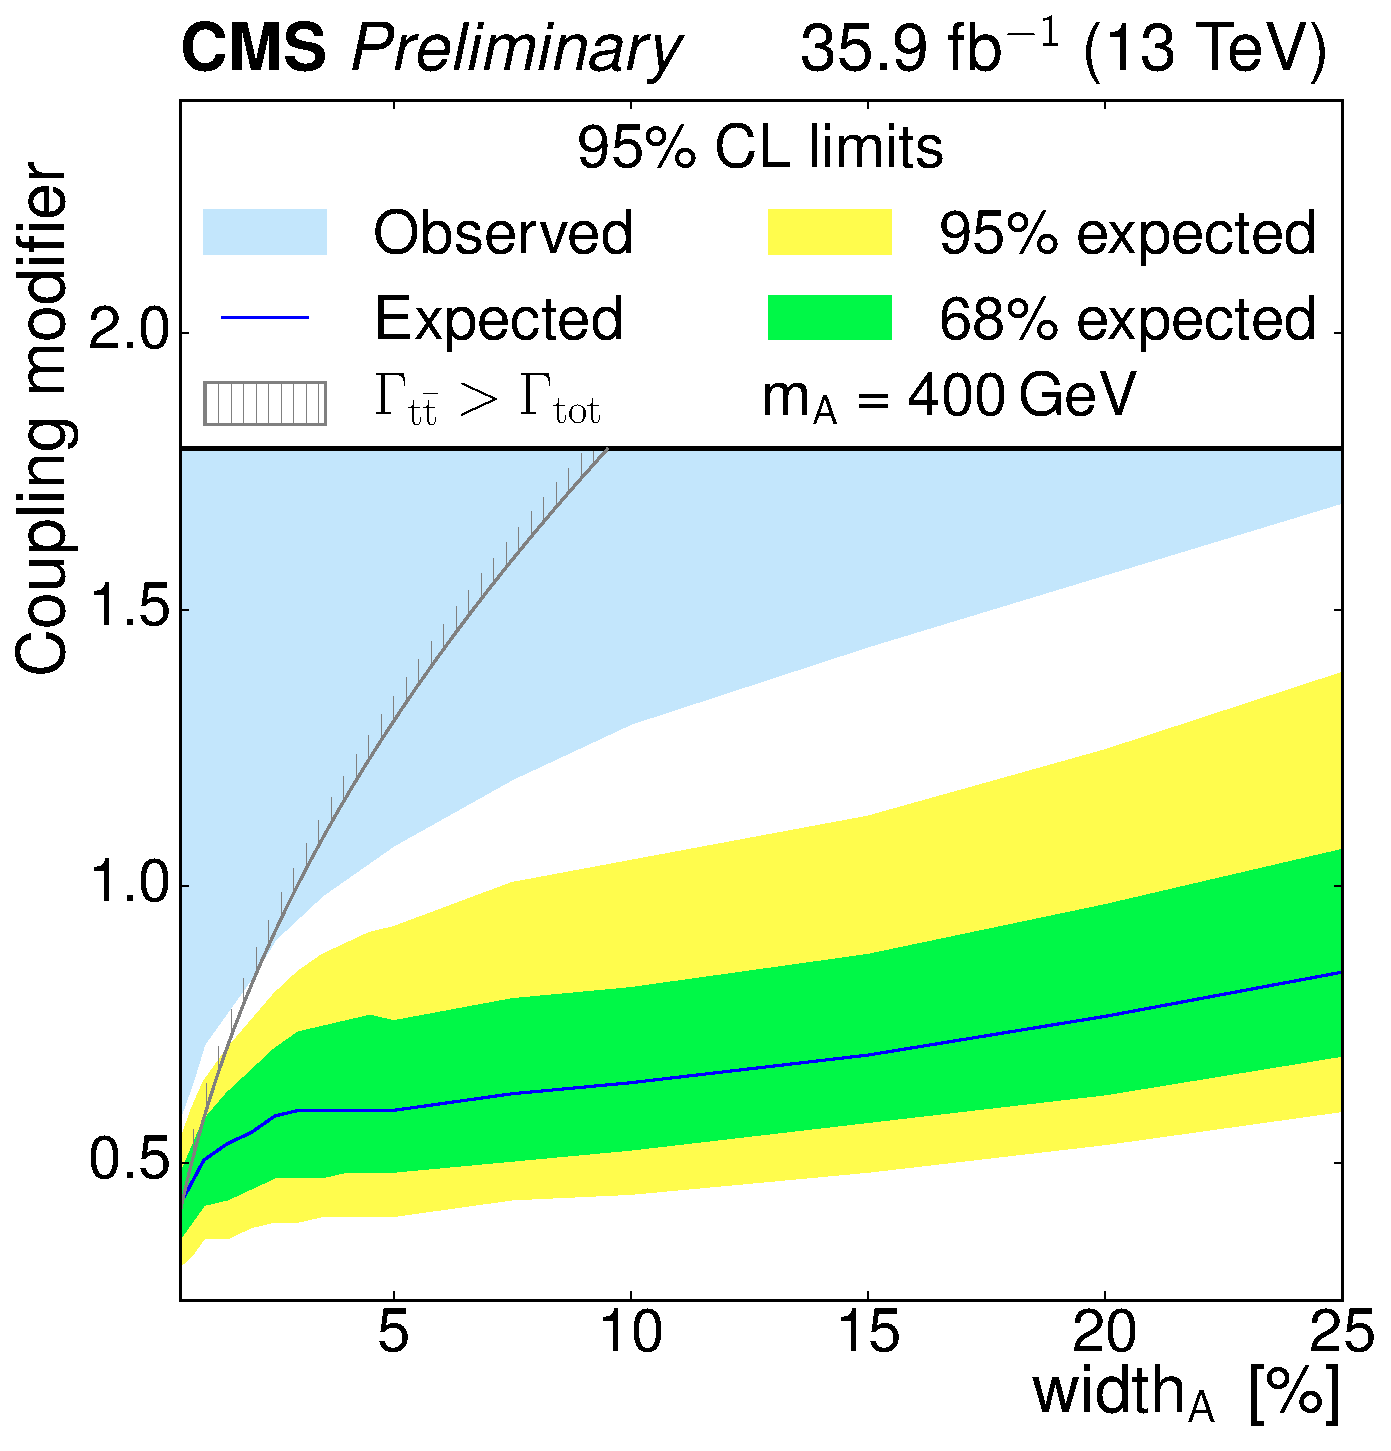
\includegraphics[width=0.35\textwidth,keepaspectratio=true]{fig/chapt8/limits/limit_A_M400.pdf}
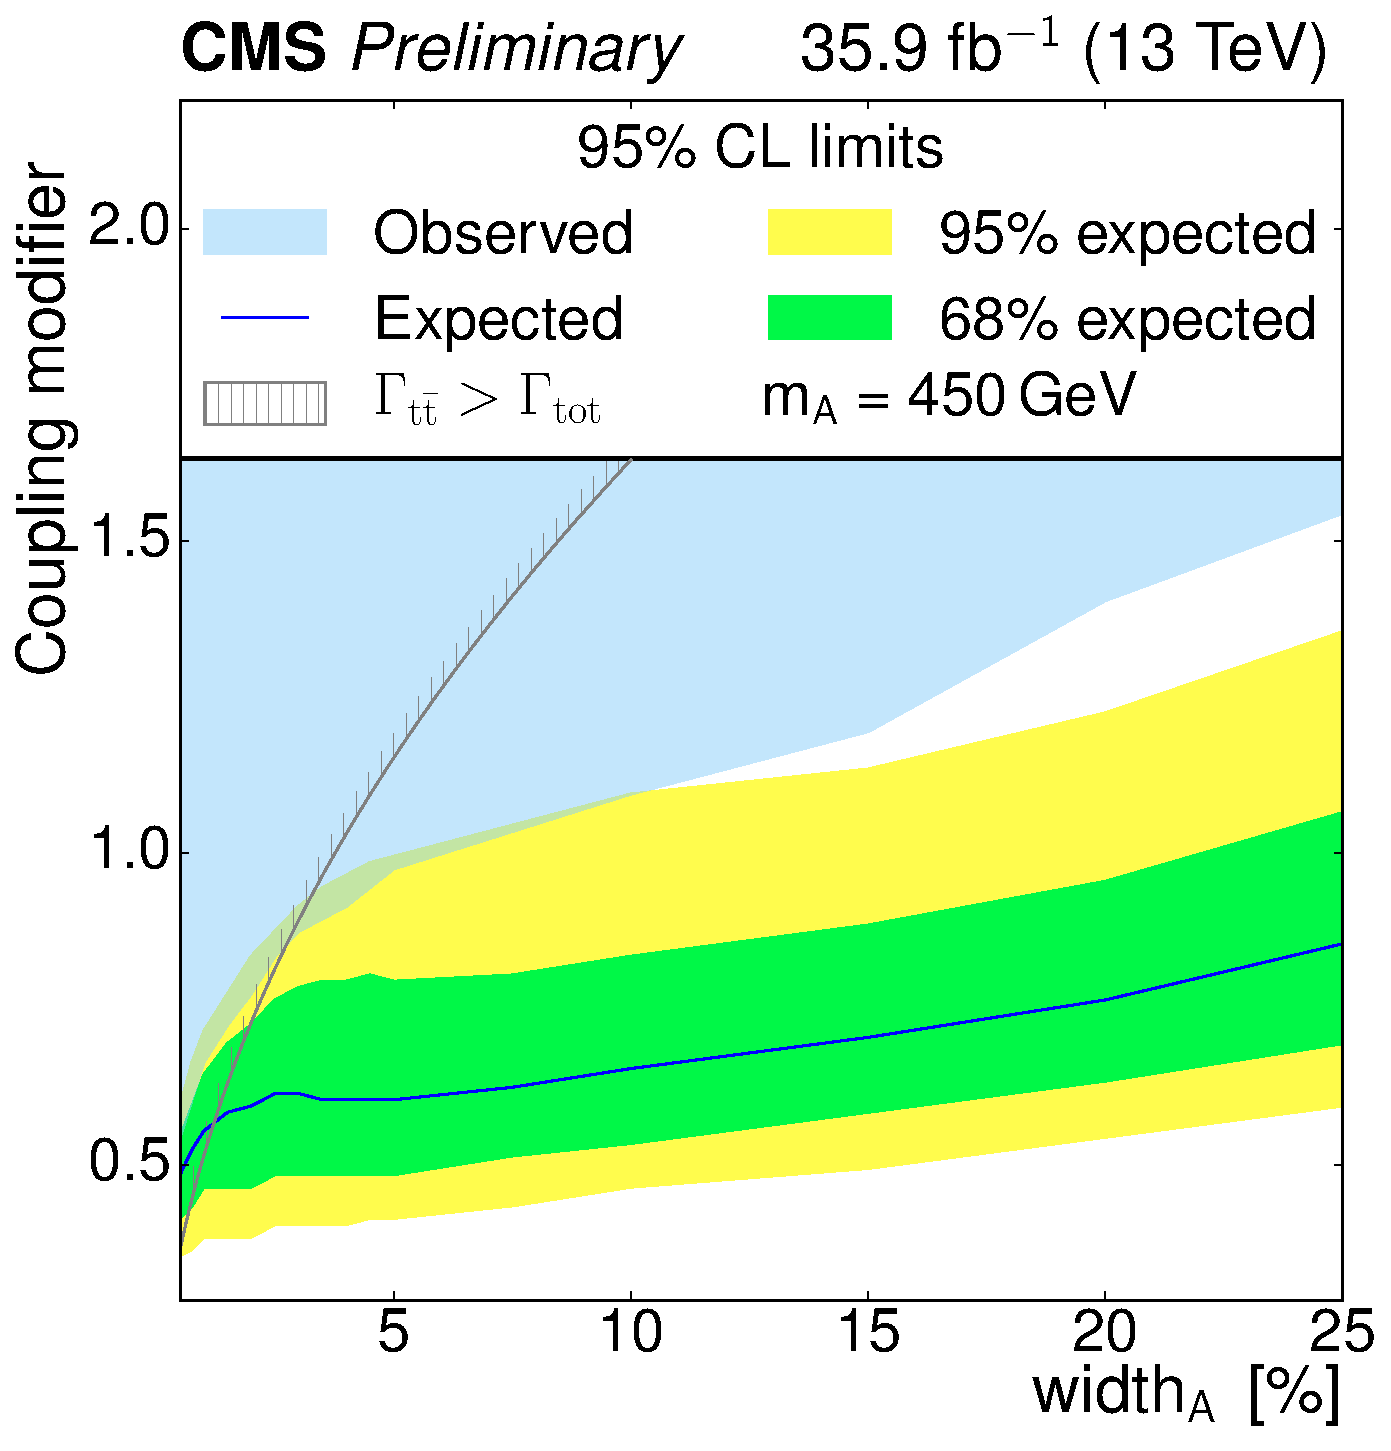
\includegraphics[width=0.35\textwidth,keepaspectratio=true]{fig/chapt8/limits/limit_A_M450.pdf}
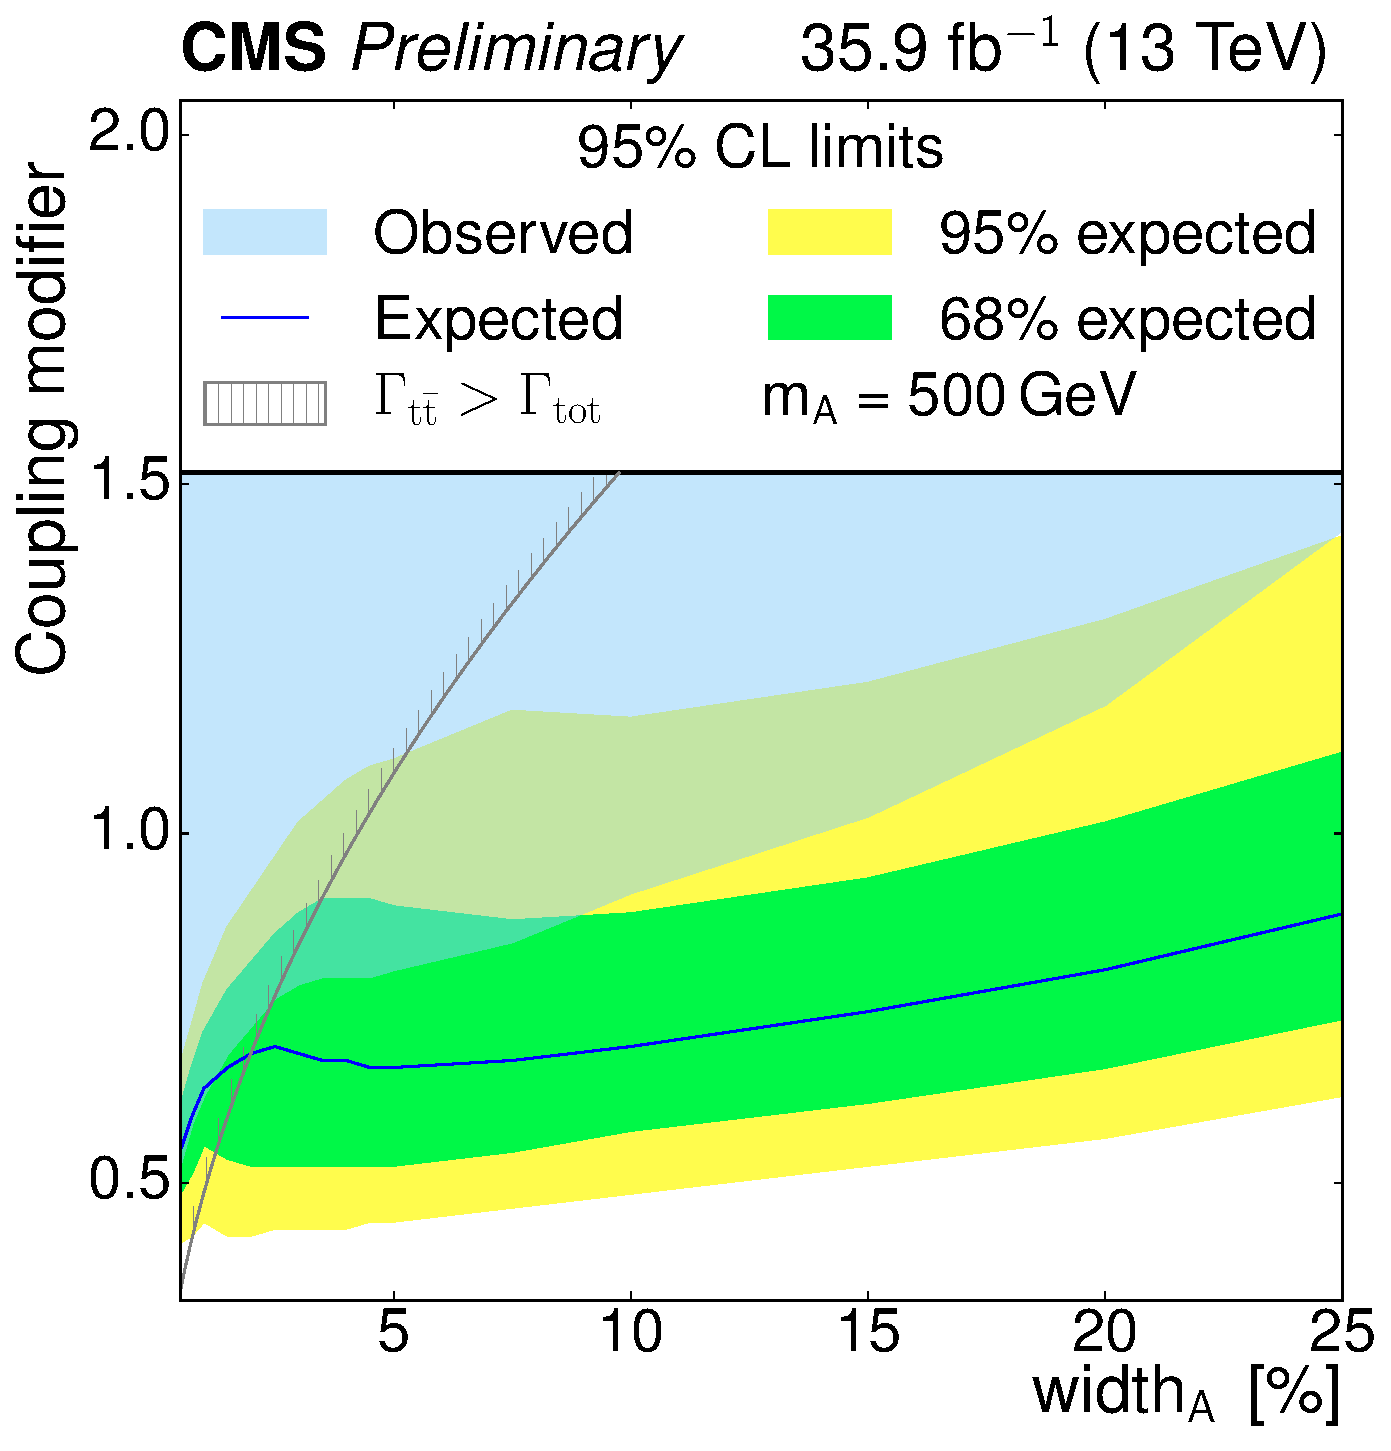
\includegraphics[width=0.35\textwidth,keepaspectratio=true]{fig/chapt8/limits/limit_A_M500.pdf}
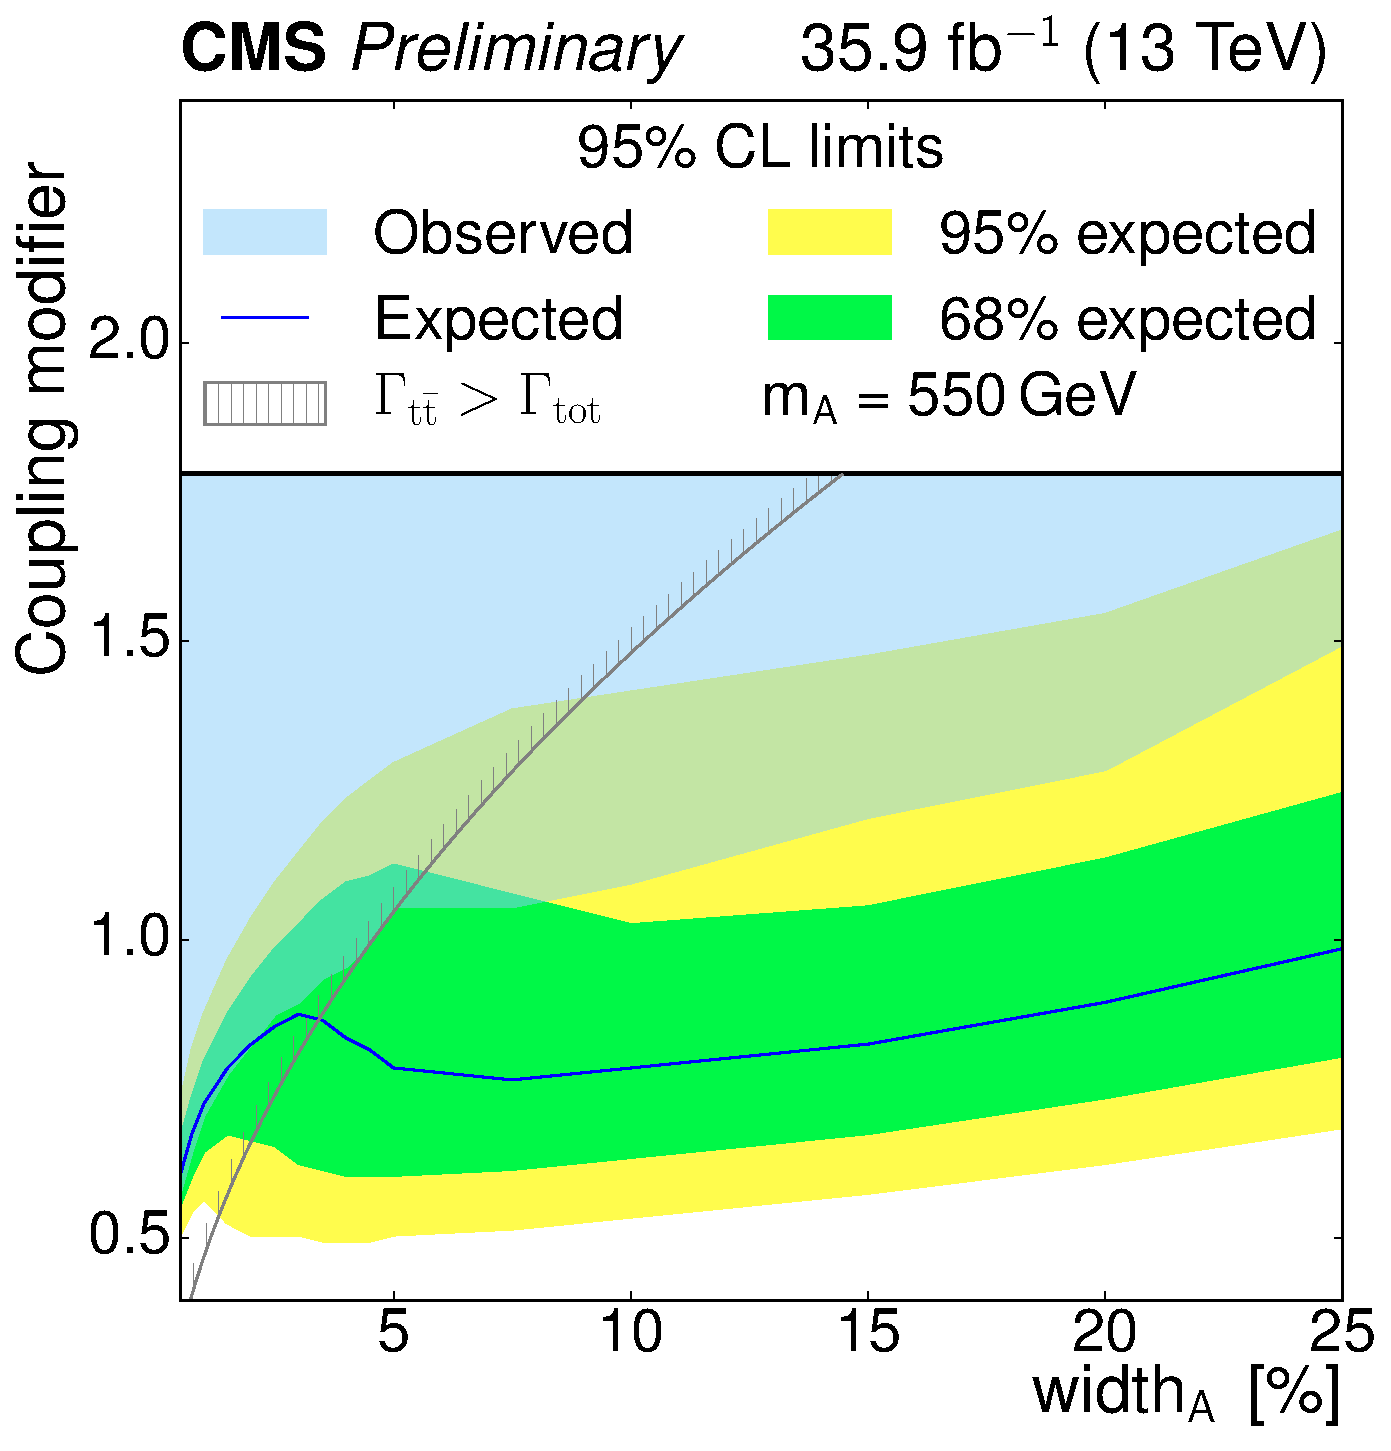
\includegraphics[width=0.35\textwidth,keepaspectratio=true]{fig/chapt8/limits/limit_A_M550.pdf}
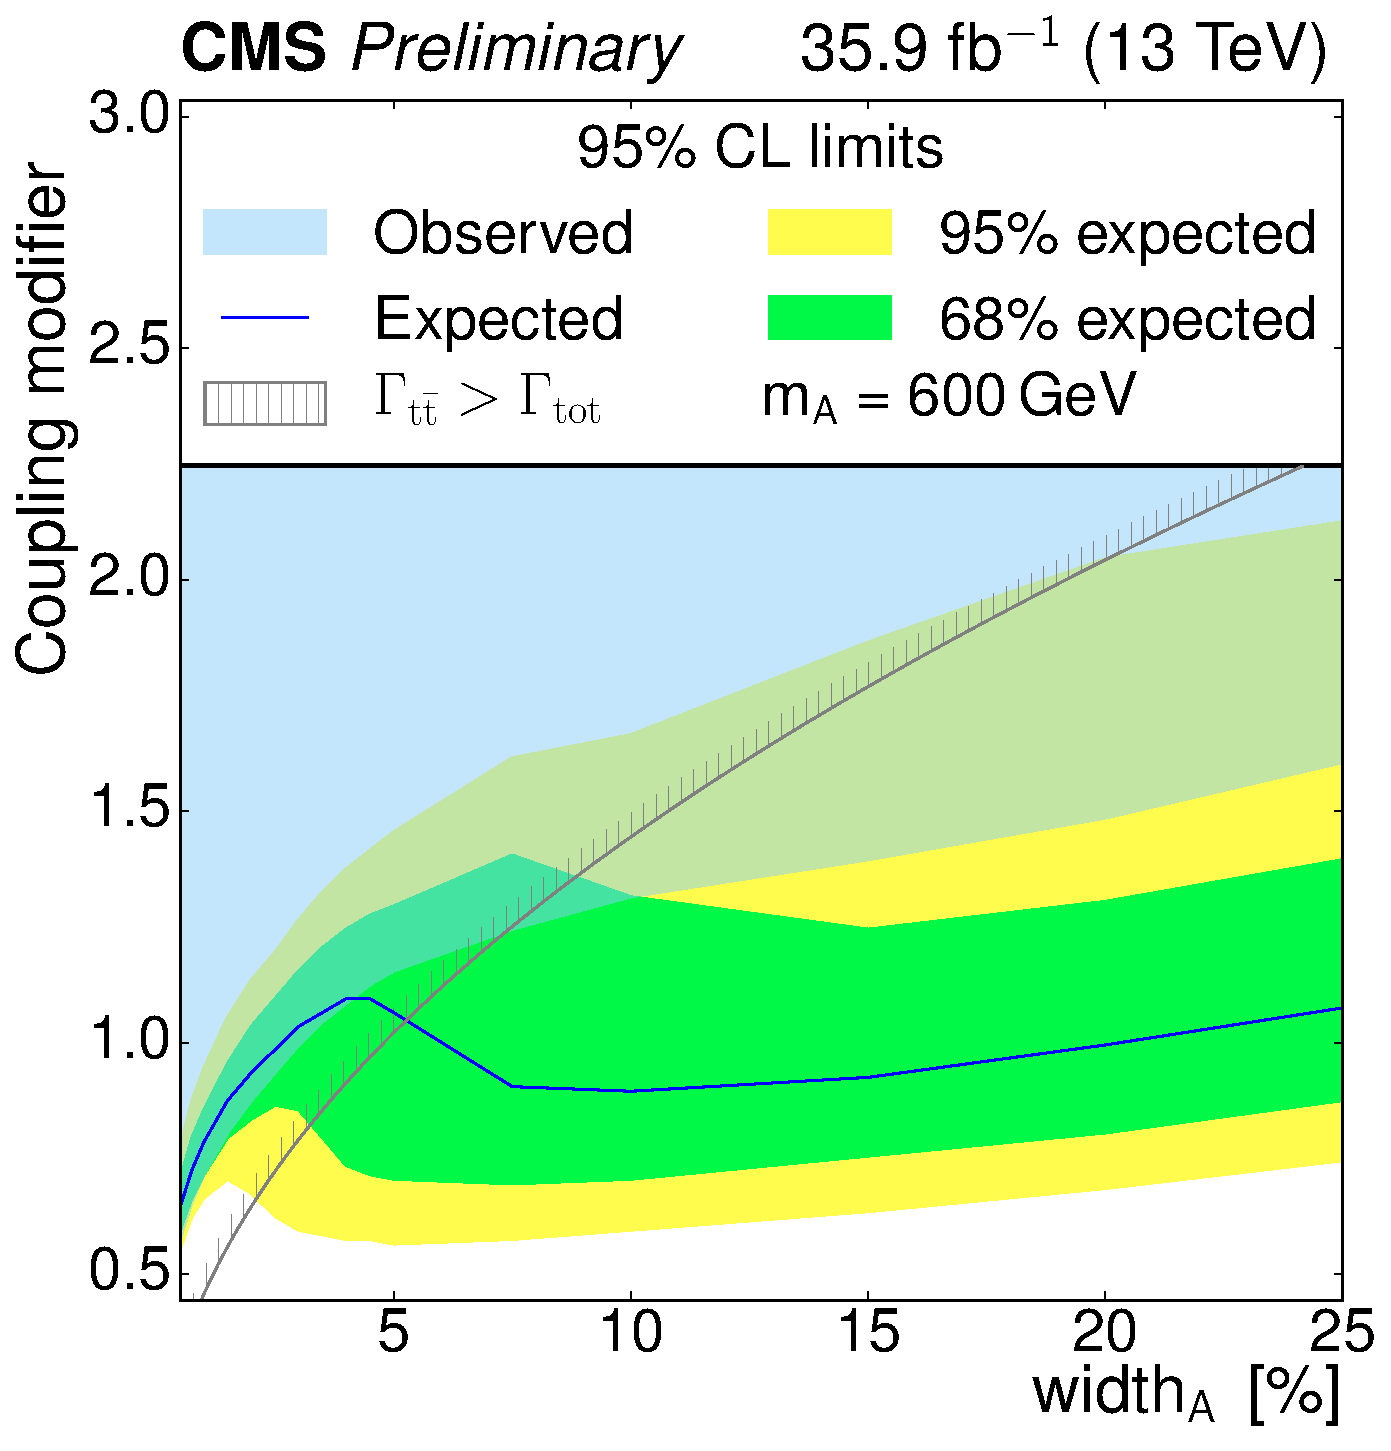
\includegraphics[width=0.35\textwidth,keepaspectratio=true]{fig/chapt8/limits/limit_A_M600.pdf}
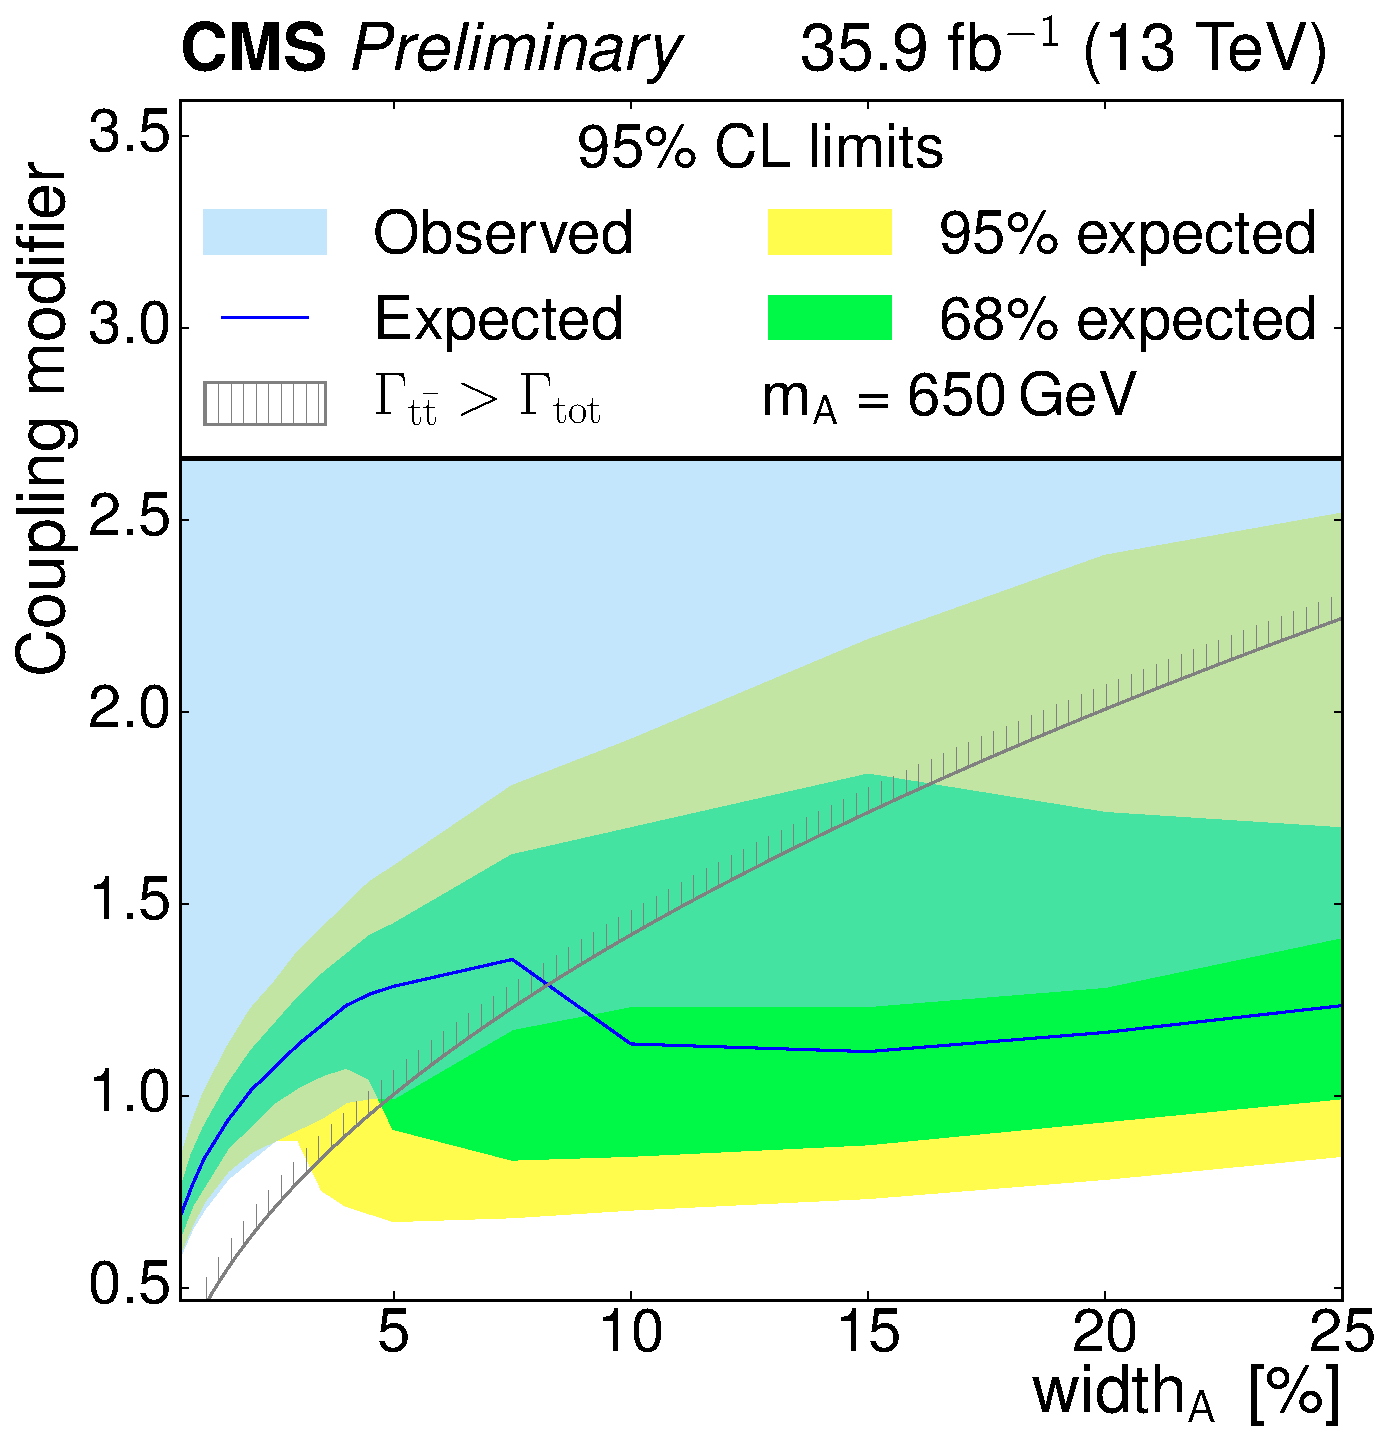
\includegraphics[width=0.35\textwidth,keepaspectratio=true]{fig/chapt8/limits/limit_A_M650.pdf}
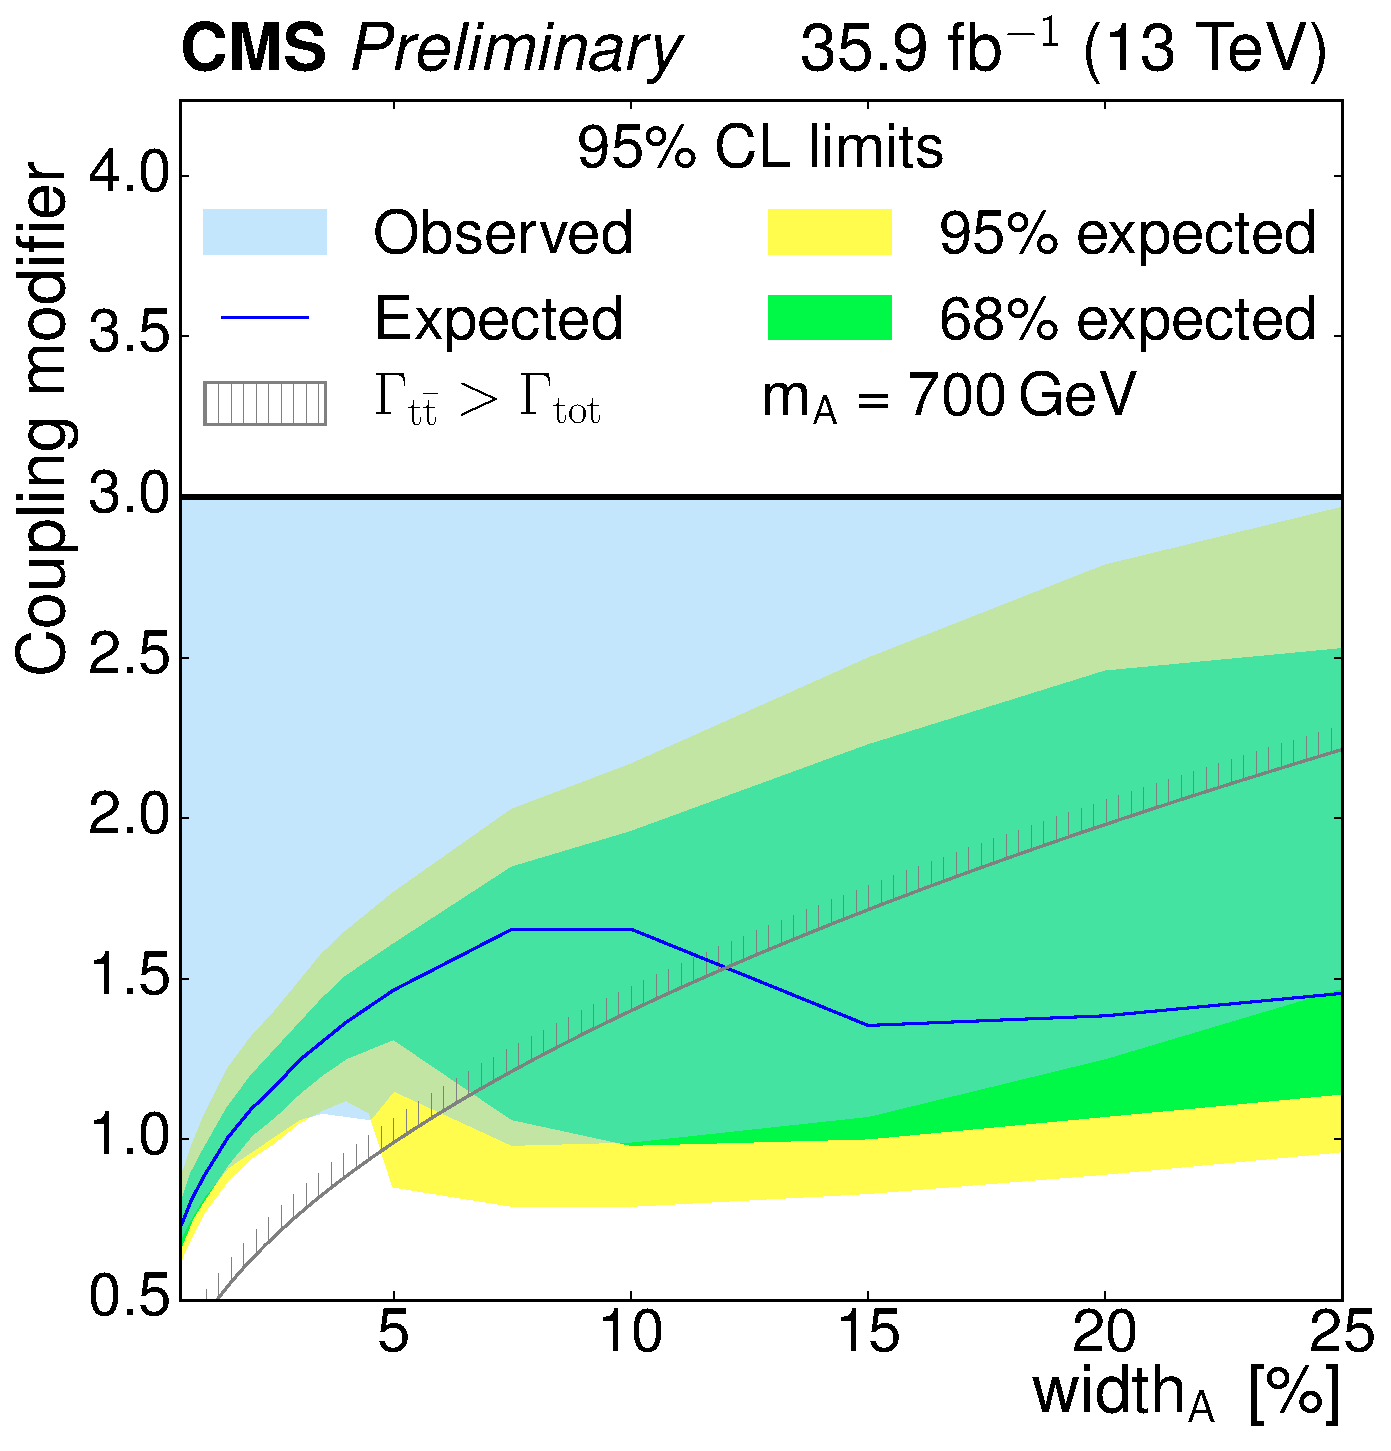
\includegraphics[width=0.35\textwidth,keepaspectratio=true]{fig/chapt8/limits/limit_A_M700.pdf}
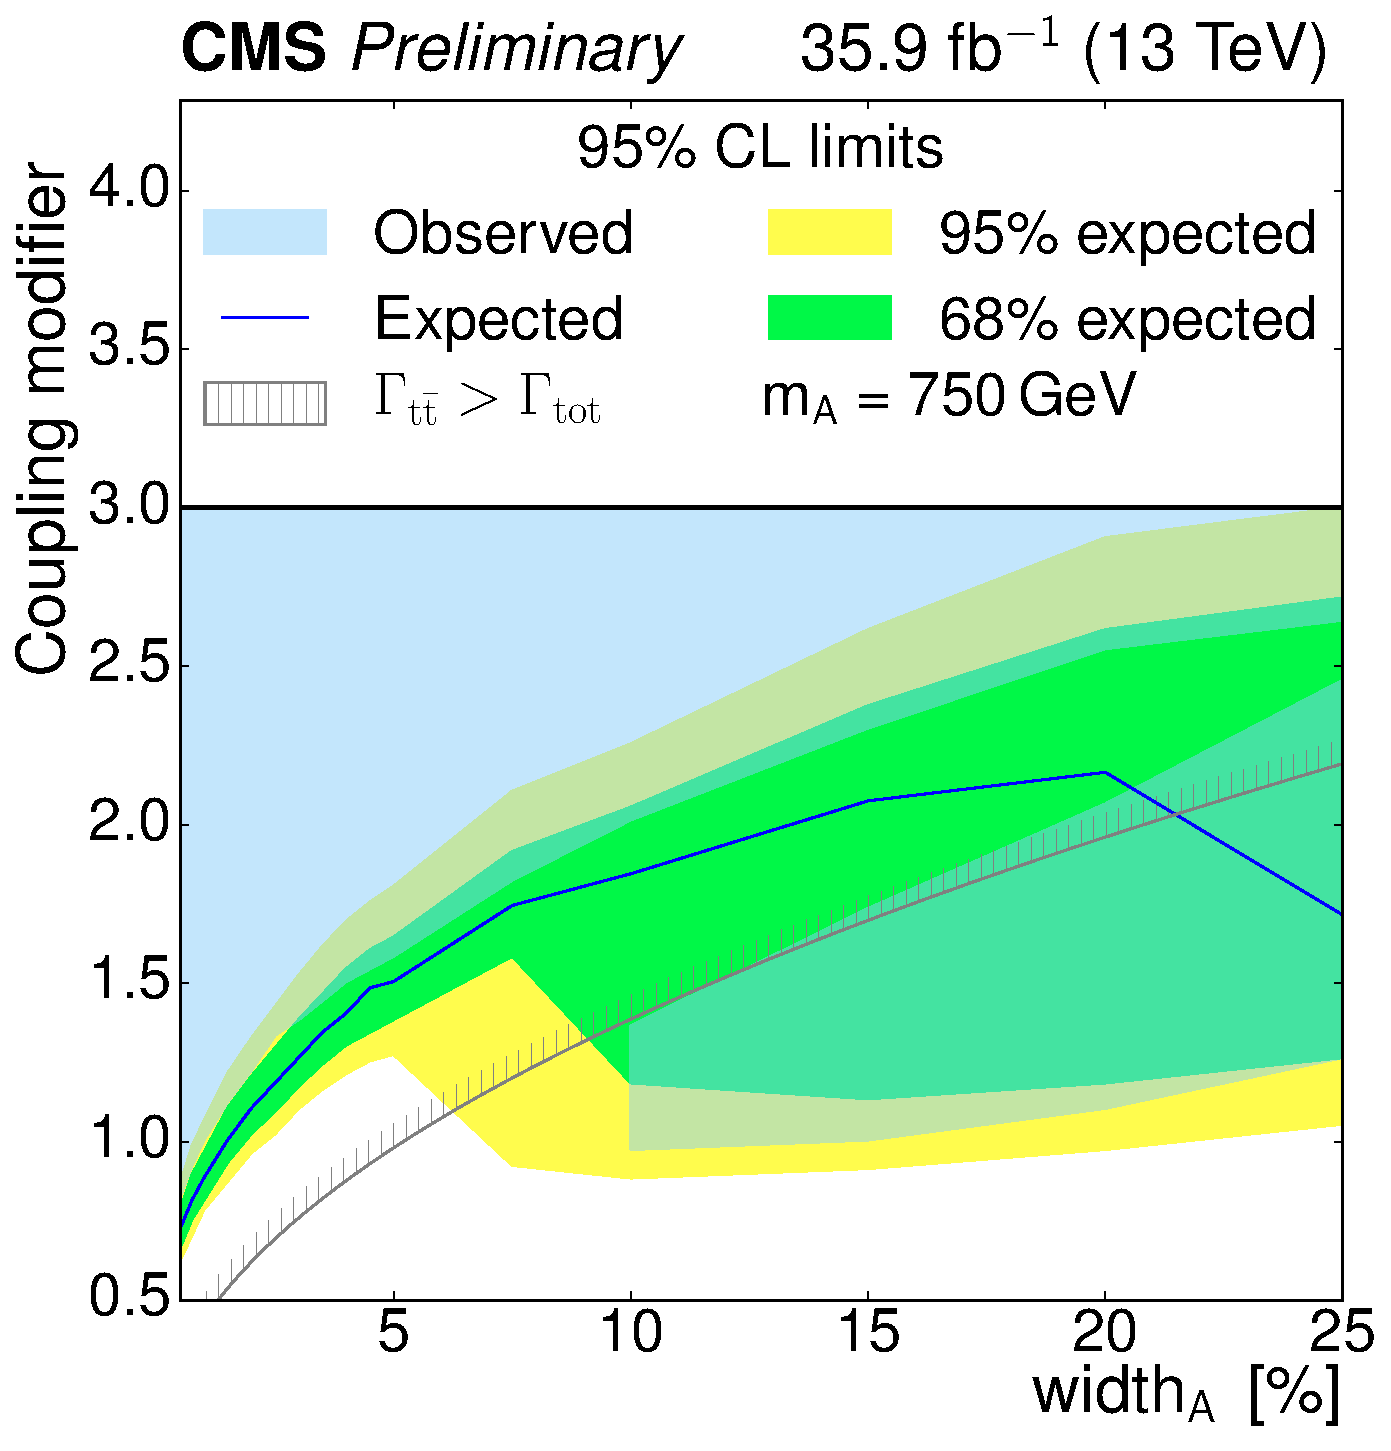
\includegraphics[width=0.35\textwidth,keepaspectratio=true]{fig/chapt8/limits/limit_A_M750.pdf}
\caption{Model-independent combined limits on the coupling strength modifier as a function of relative width for masses between 400 and 750\,GeV in steps of 50\,GeV. The limits are derived for pseudoscalar signal only. The observed limits are shown by the blue shaded area. The inner (green) band and the outer (yellow) band indicate the regions containing 68 and 95\%, respectively, of the distribution of limits expected under the background-only hypothesis. The region of phase space in which $\Gamma_{t\bar t}>\Gamma_\mathrm{tot}$ is indicated by the hatched lines.}
\label{fig:limits_a_masses}
\end{figure}

\begin{figure}[!Hhtb]
\centering
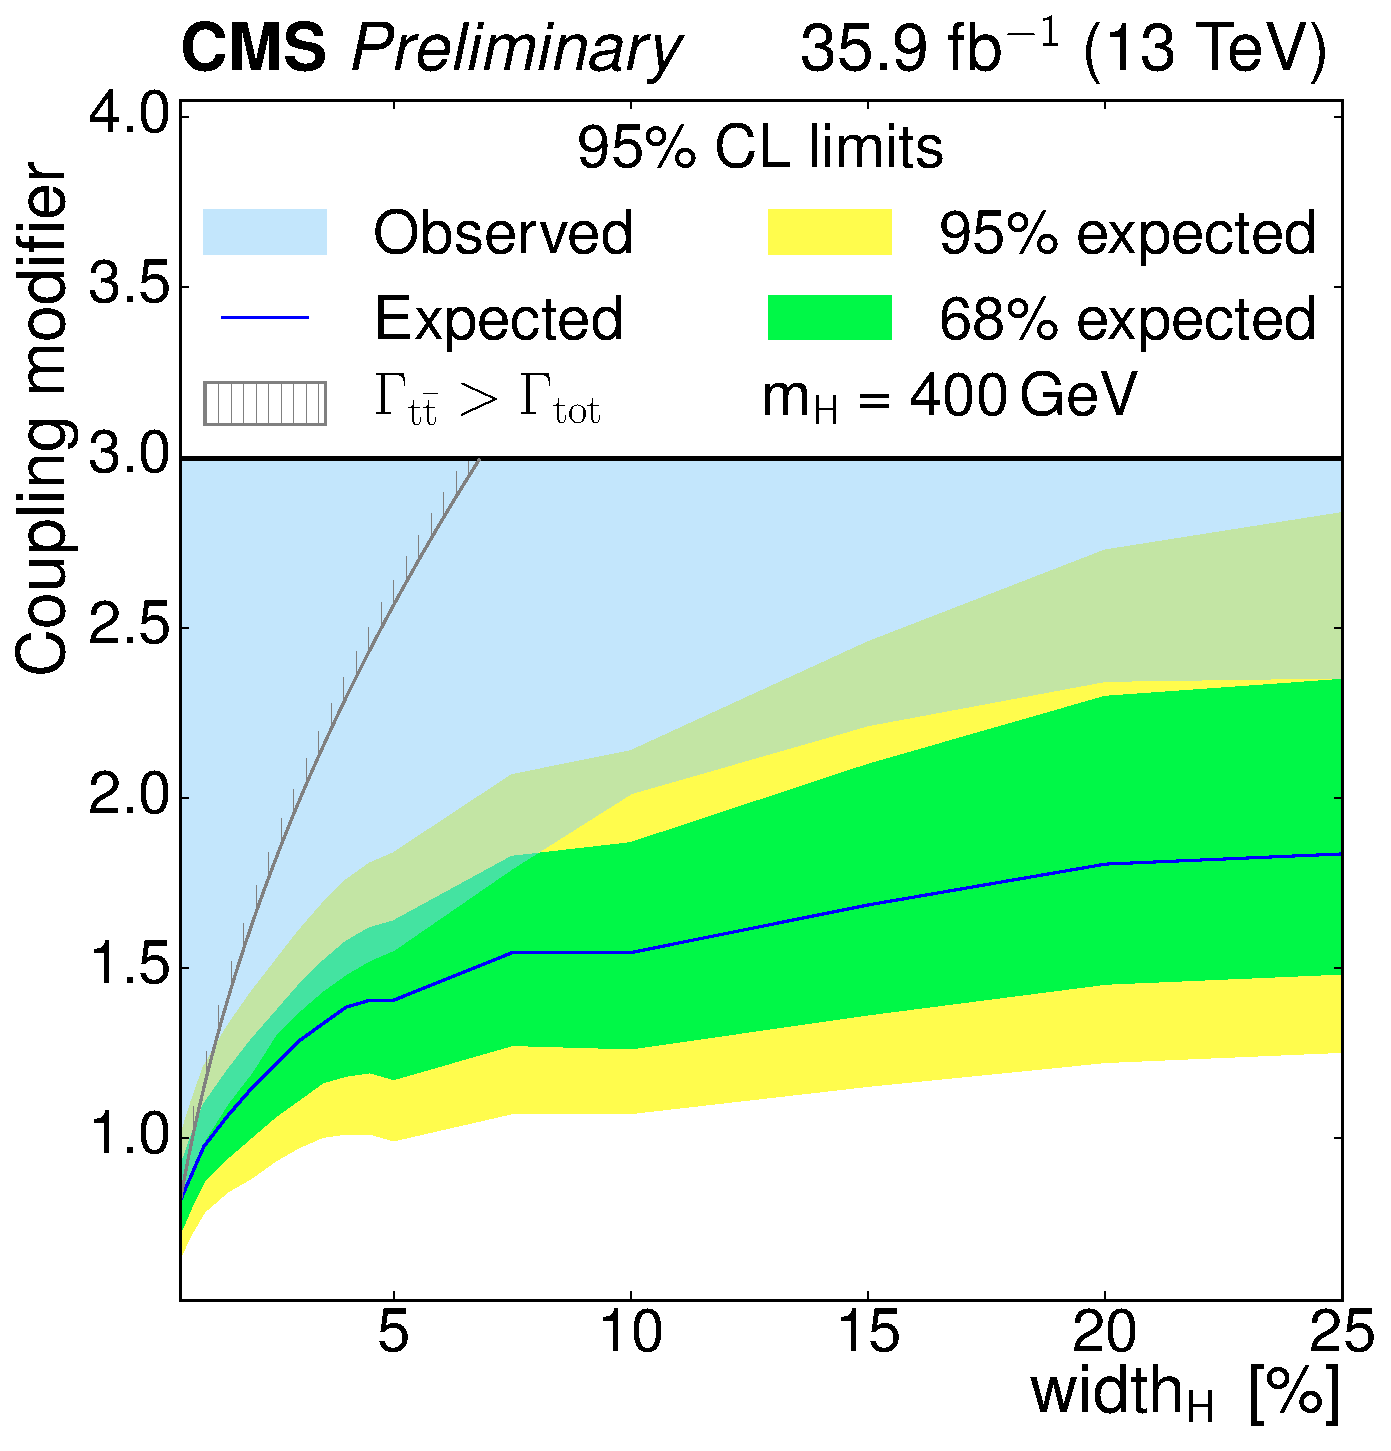
\includegraphics[width=0.35\textwidth,keepaspectratio=true]{fig/chapt8/limits/limit_H_M400.pdf}
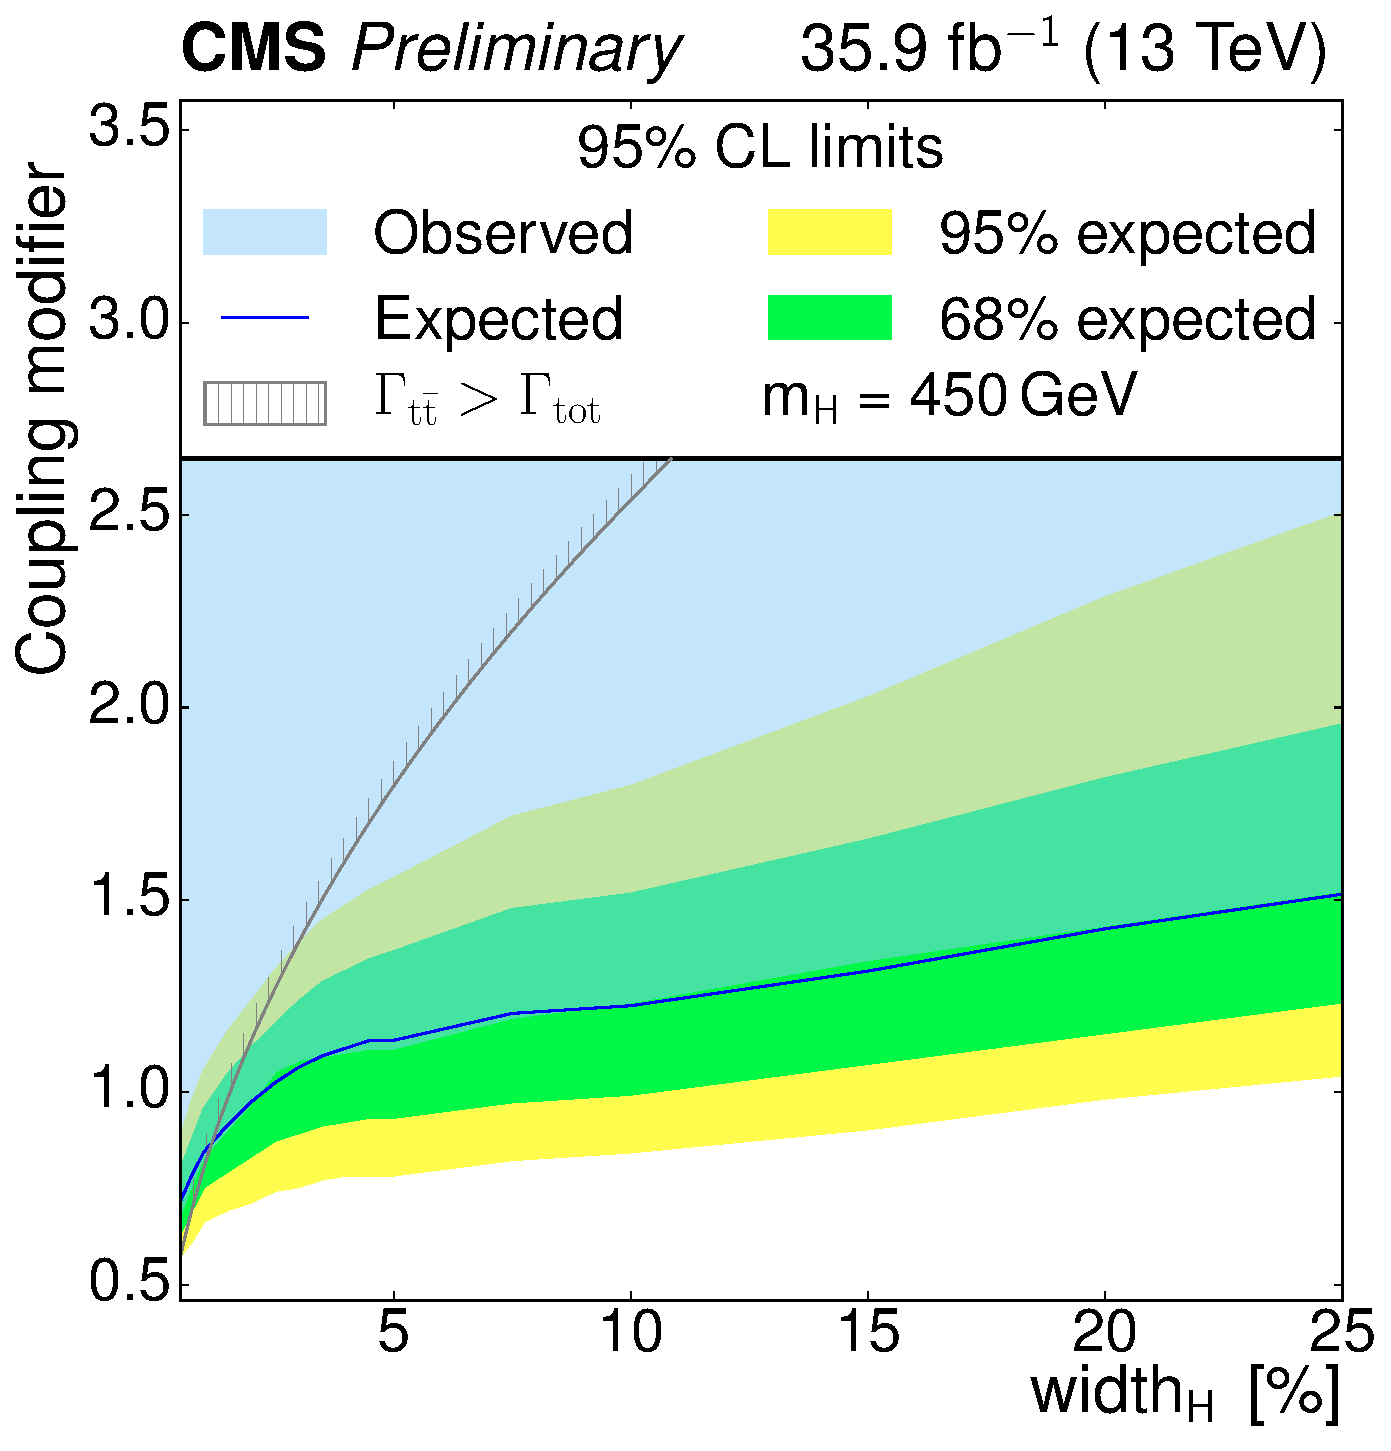
\includegraphics[width=0.35\textwidth,keepaspectratio=true]{fig/chapt8/limits/limit_H_M450.pdf}
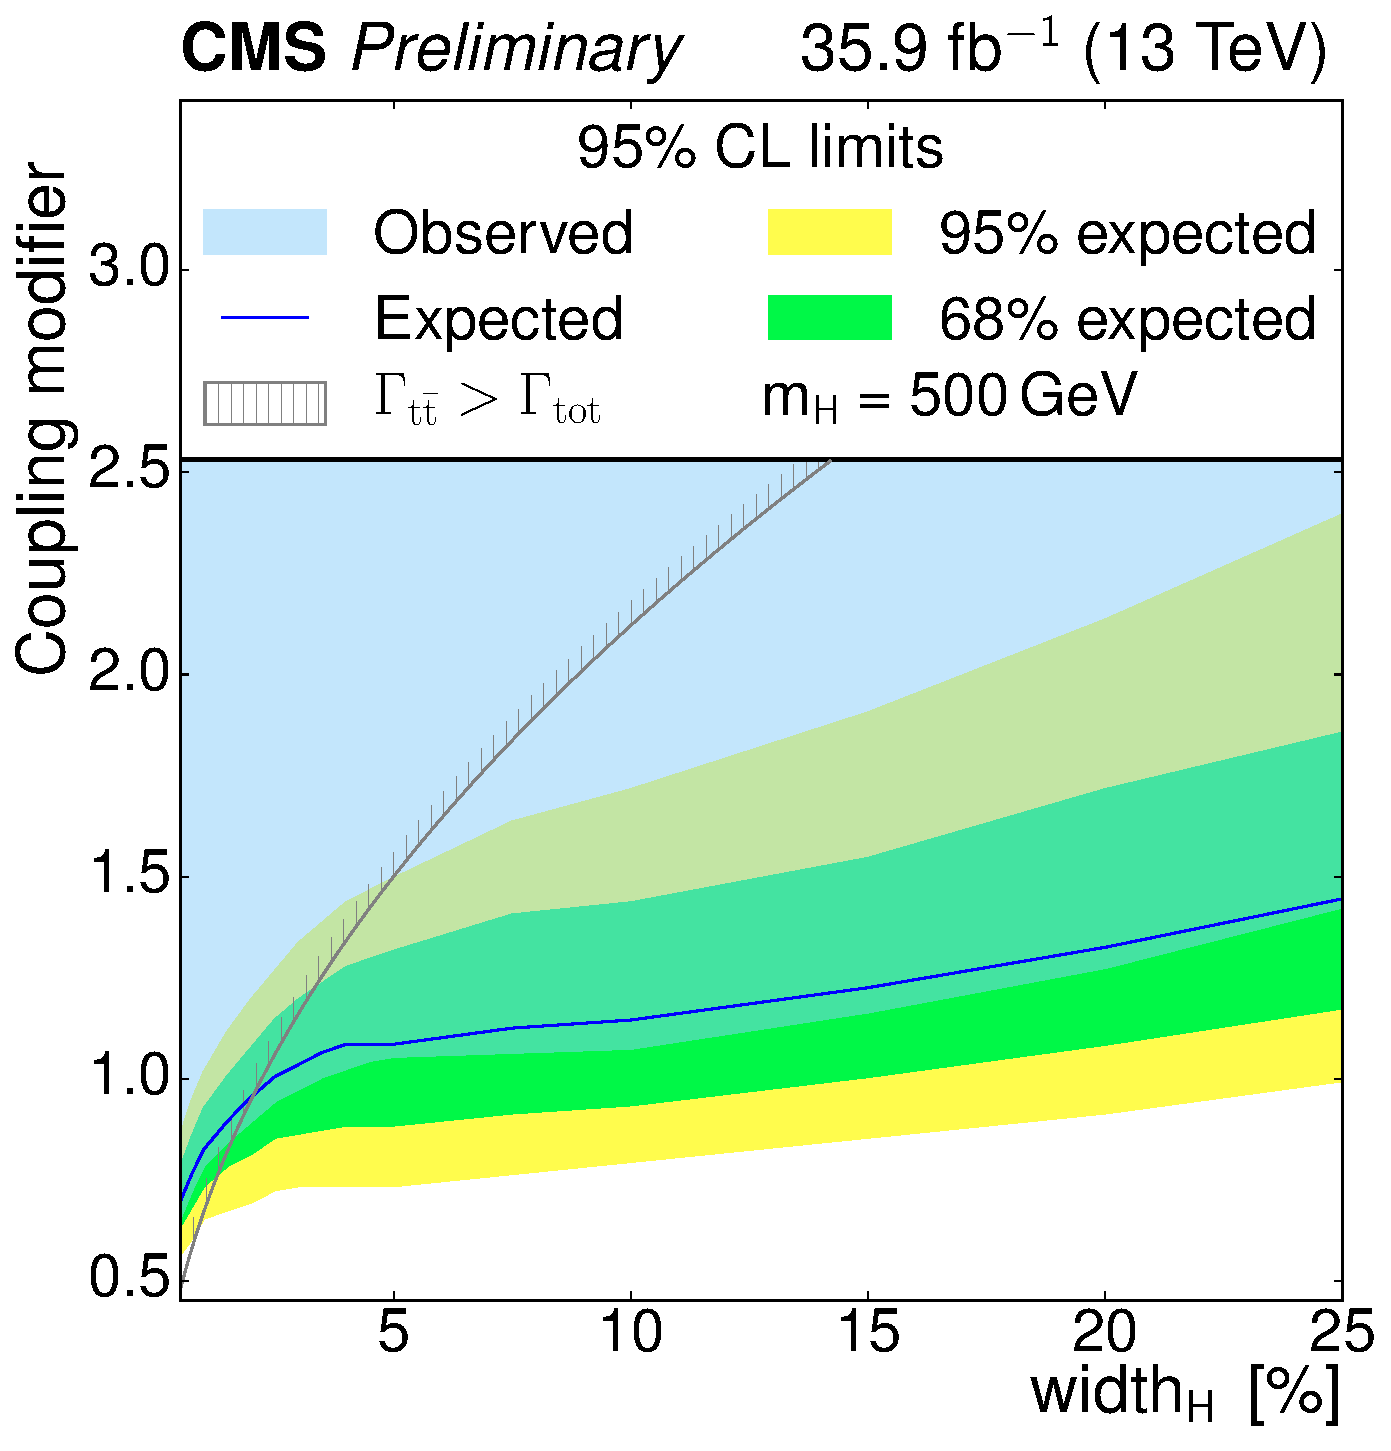
\includegraphics[width=0.35\textwidth,keepaspectratio=true]{fig/chapt8/limits/limit_H_M500.pdf}
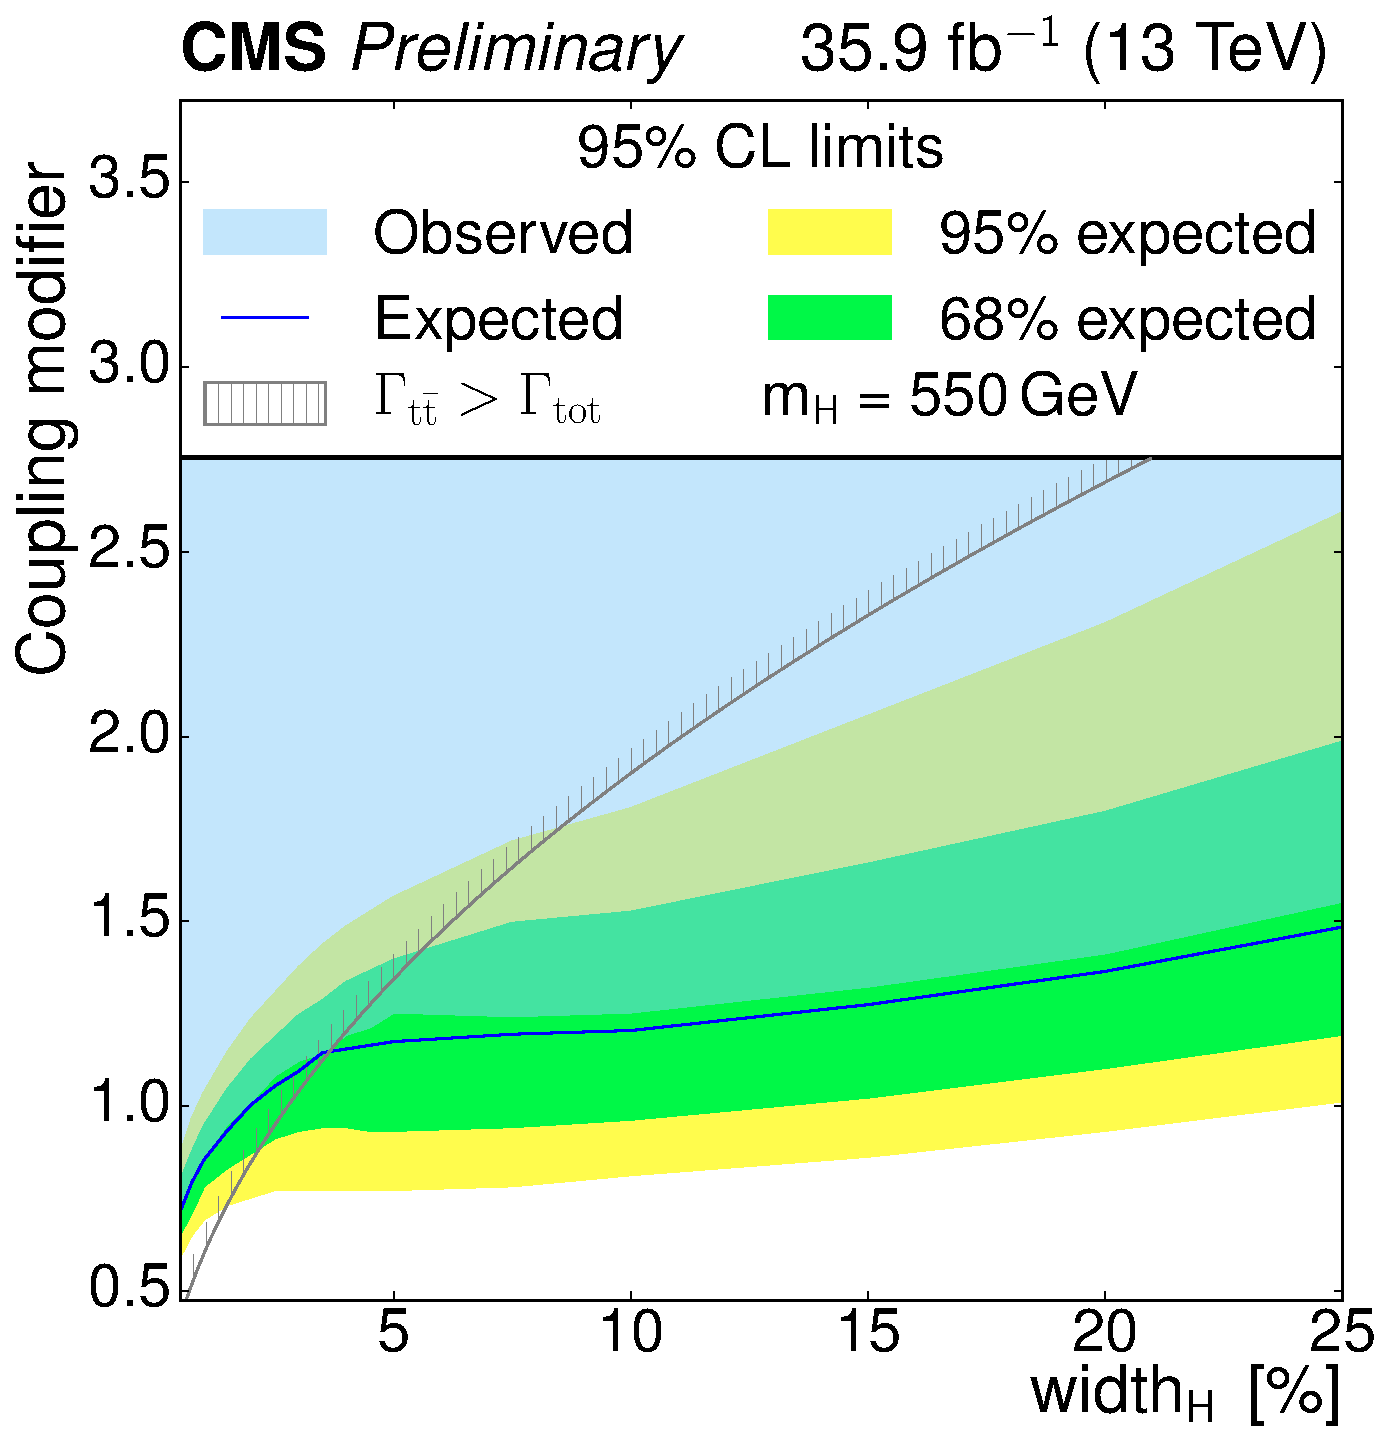
\includegraphics[width=0.35\textwidth,keepaspectratio=true]{fig/chapt8/limits/limit_H_M550.pdf}
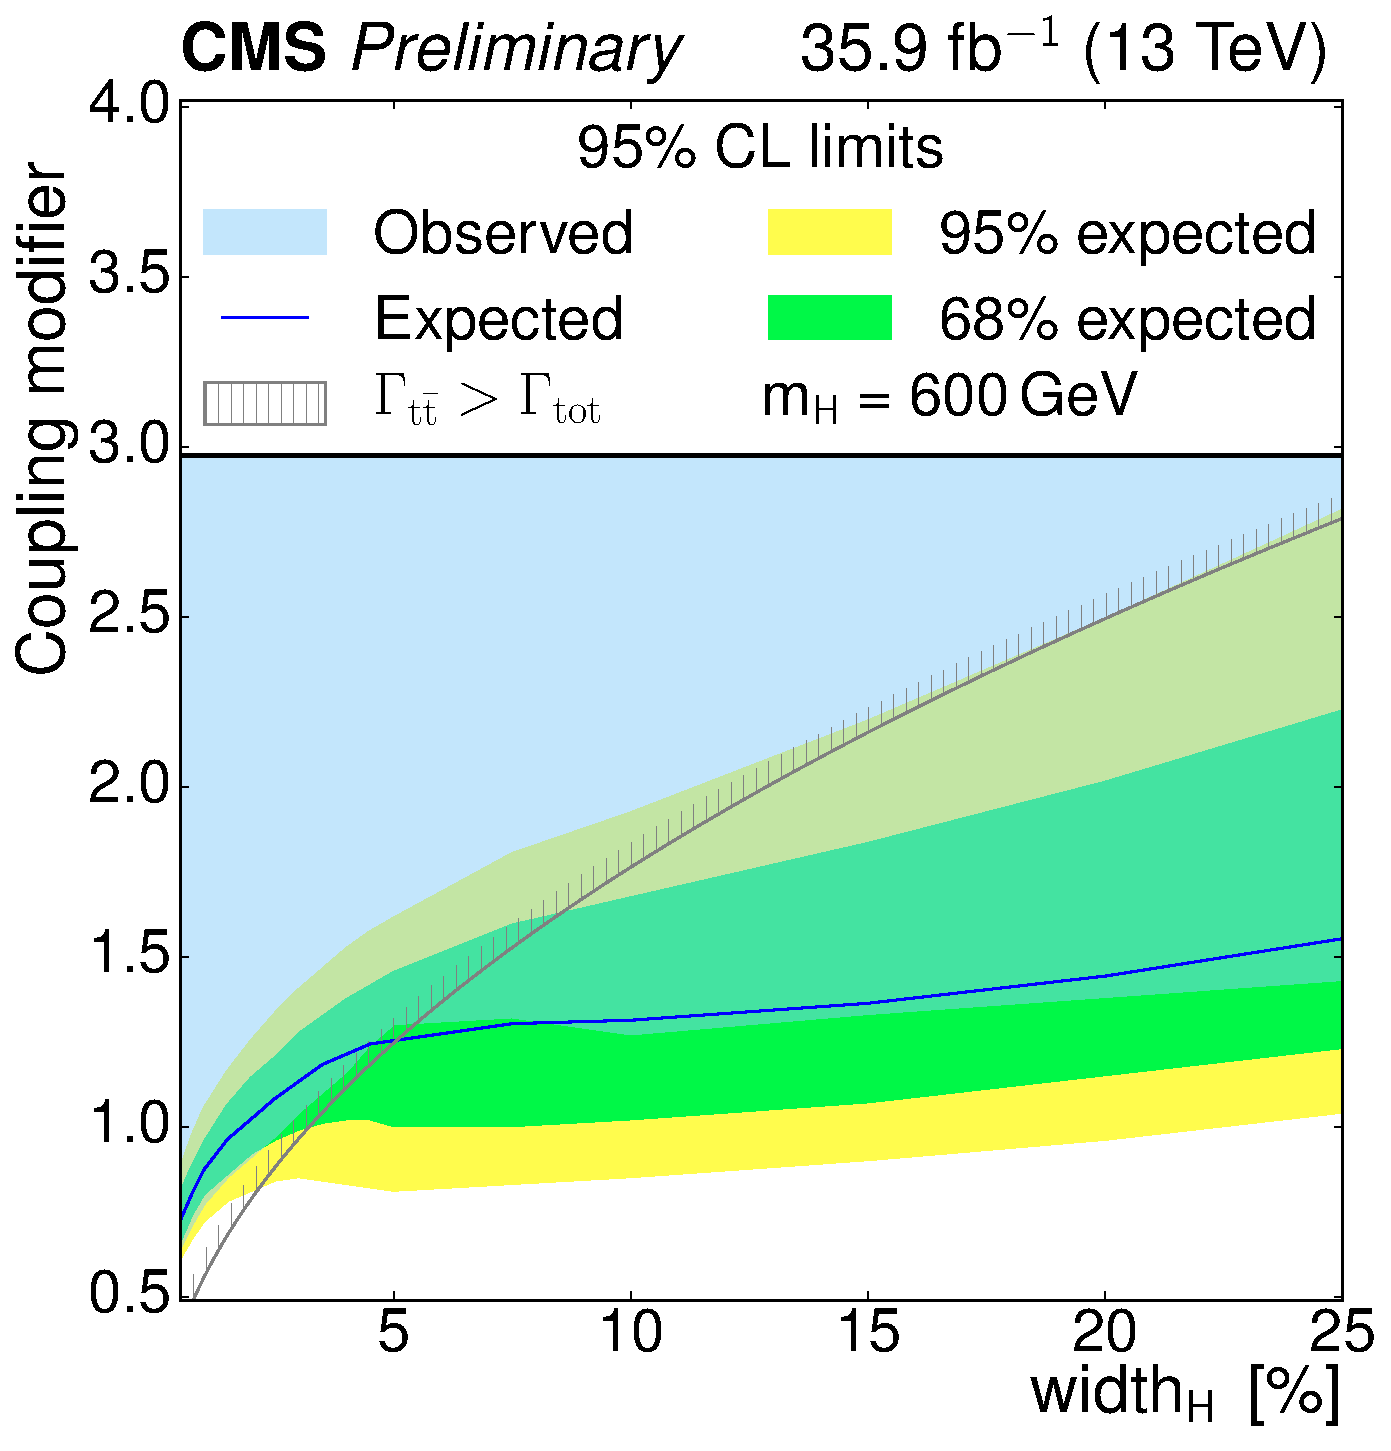
\includegraphics[width=0.35\textwidth,keepaspectratio=true]{fig/chapt8/limits/limit_H_M600.pdf}
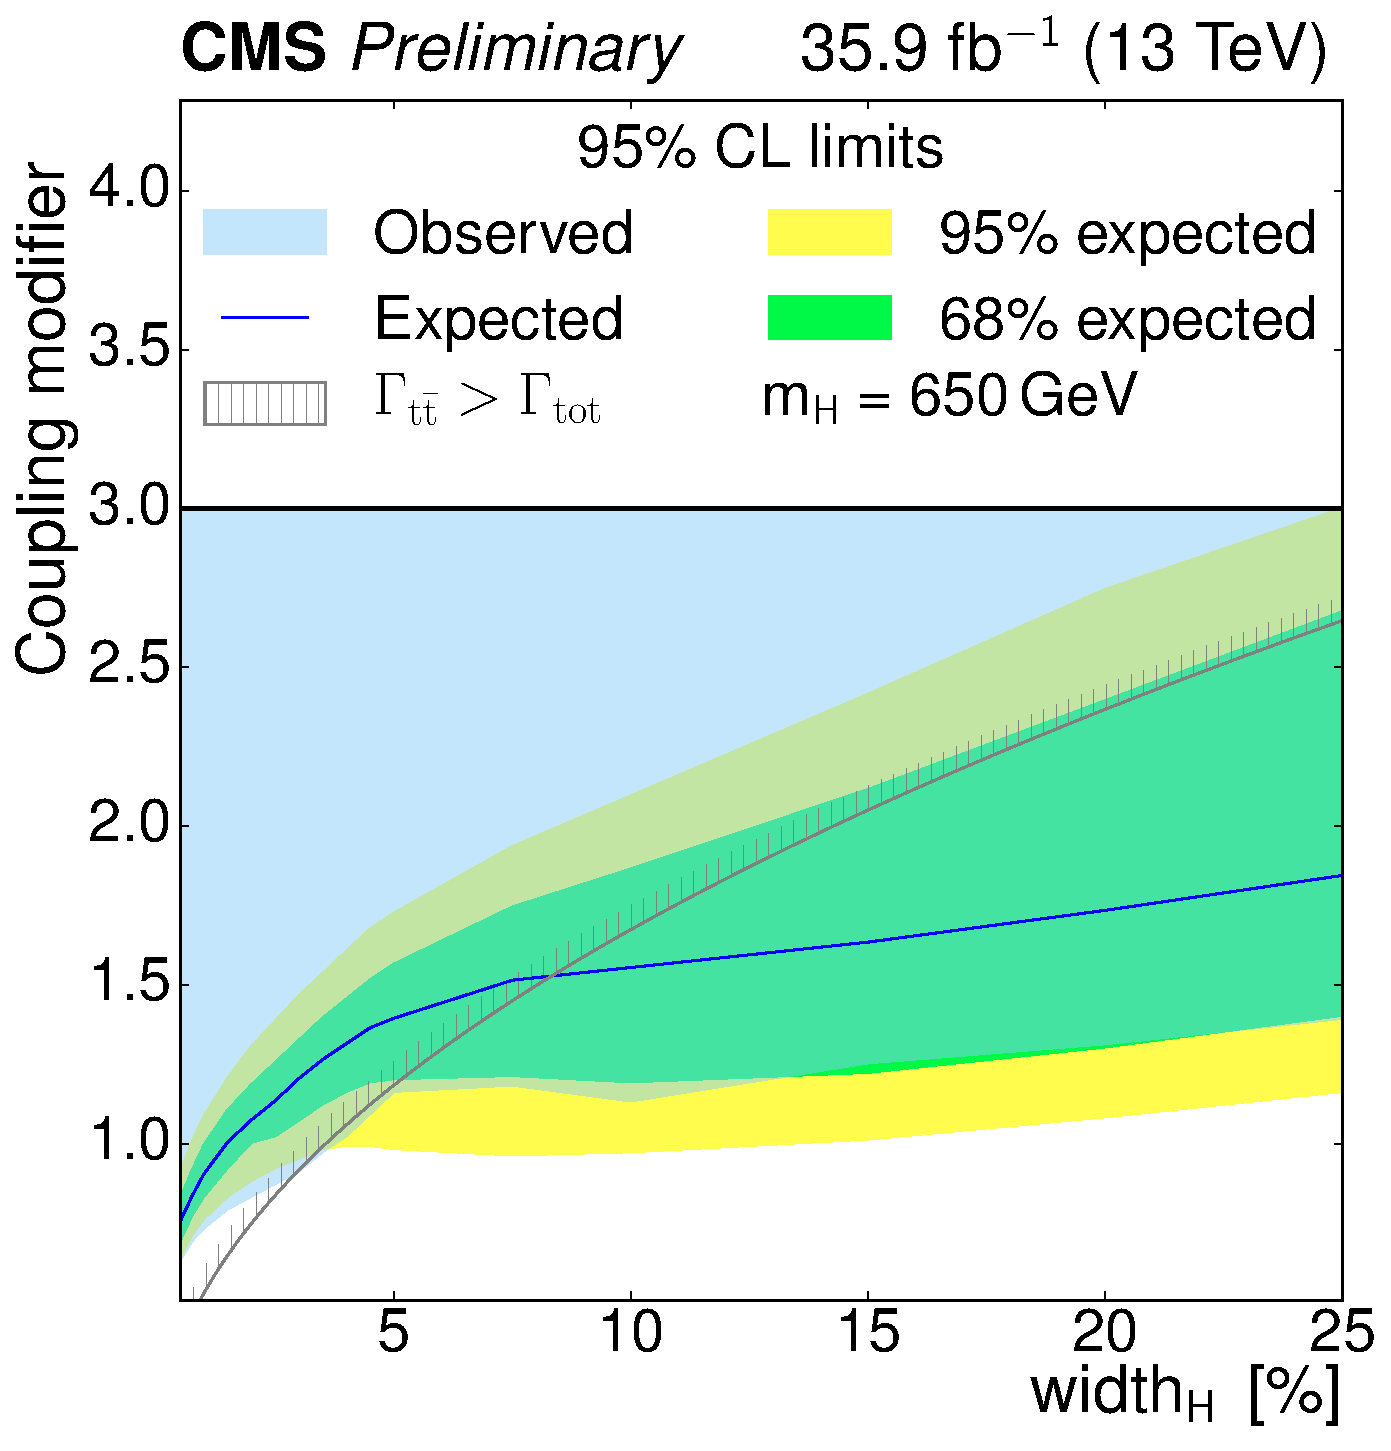
\includegraphics[width=0.35\textwidth,keepaspectratio=true]{fig/chapt8/limits/limit_H_M650.pdf}
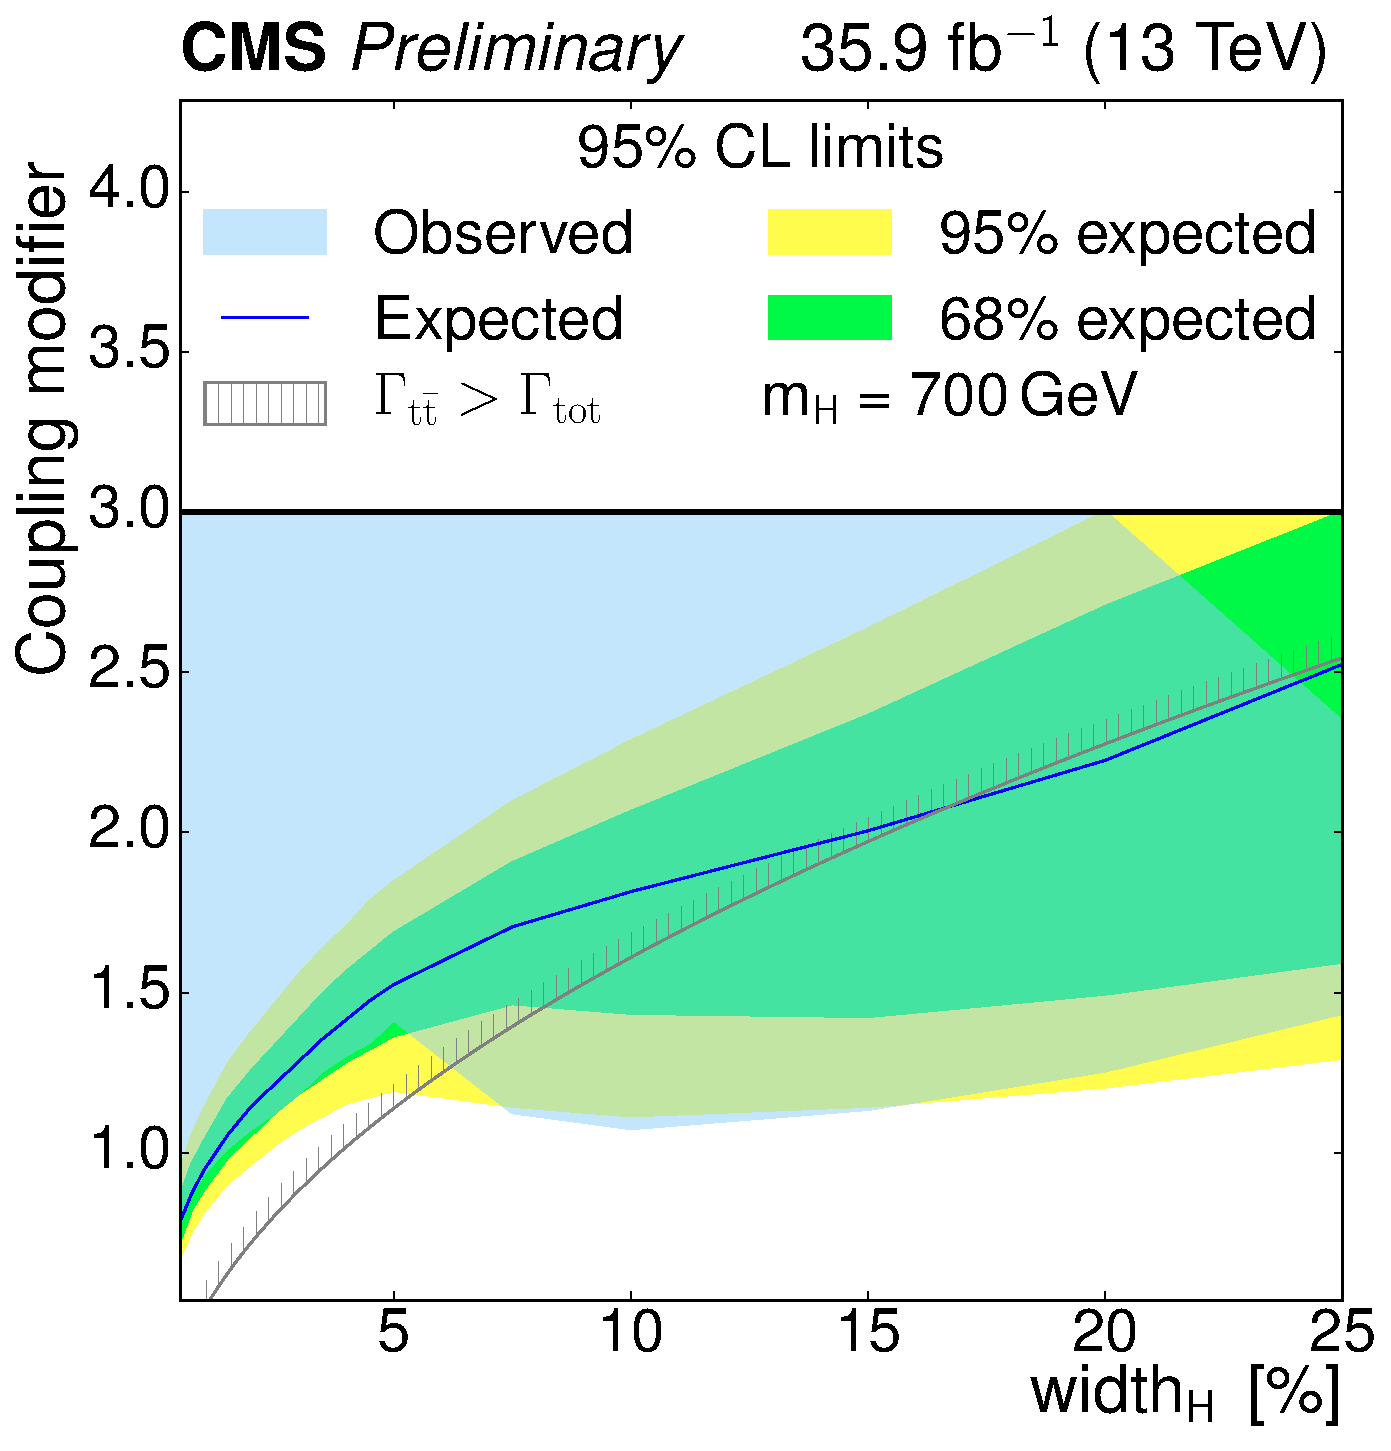
\includegraphics[width=0.35\textwidth,keepaspectratio=true]{fig/chapt8/limits/limit_H_M700.pdf}
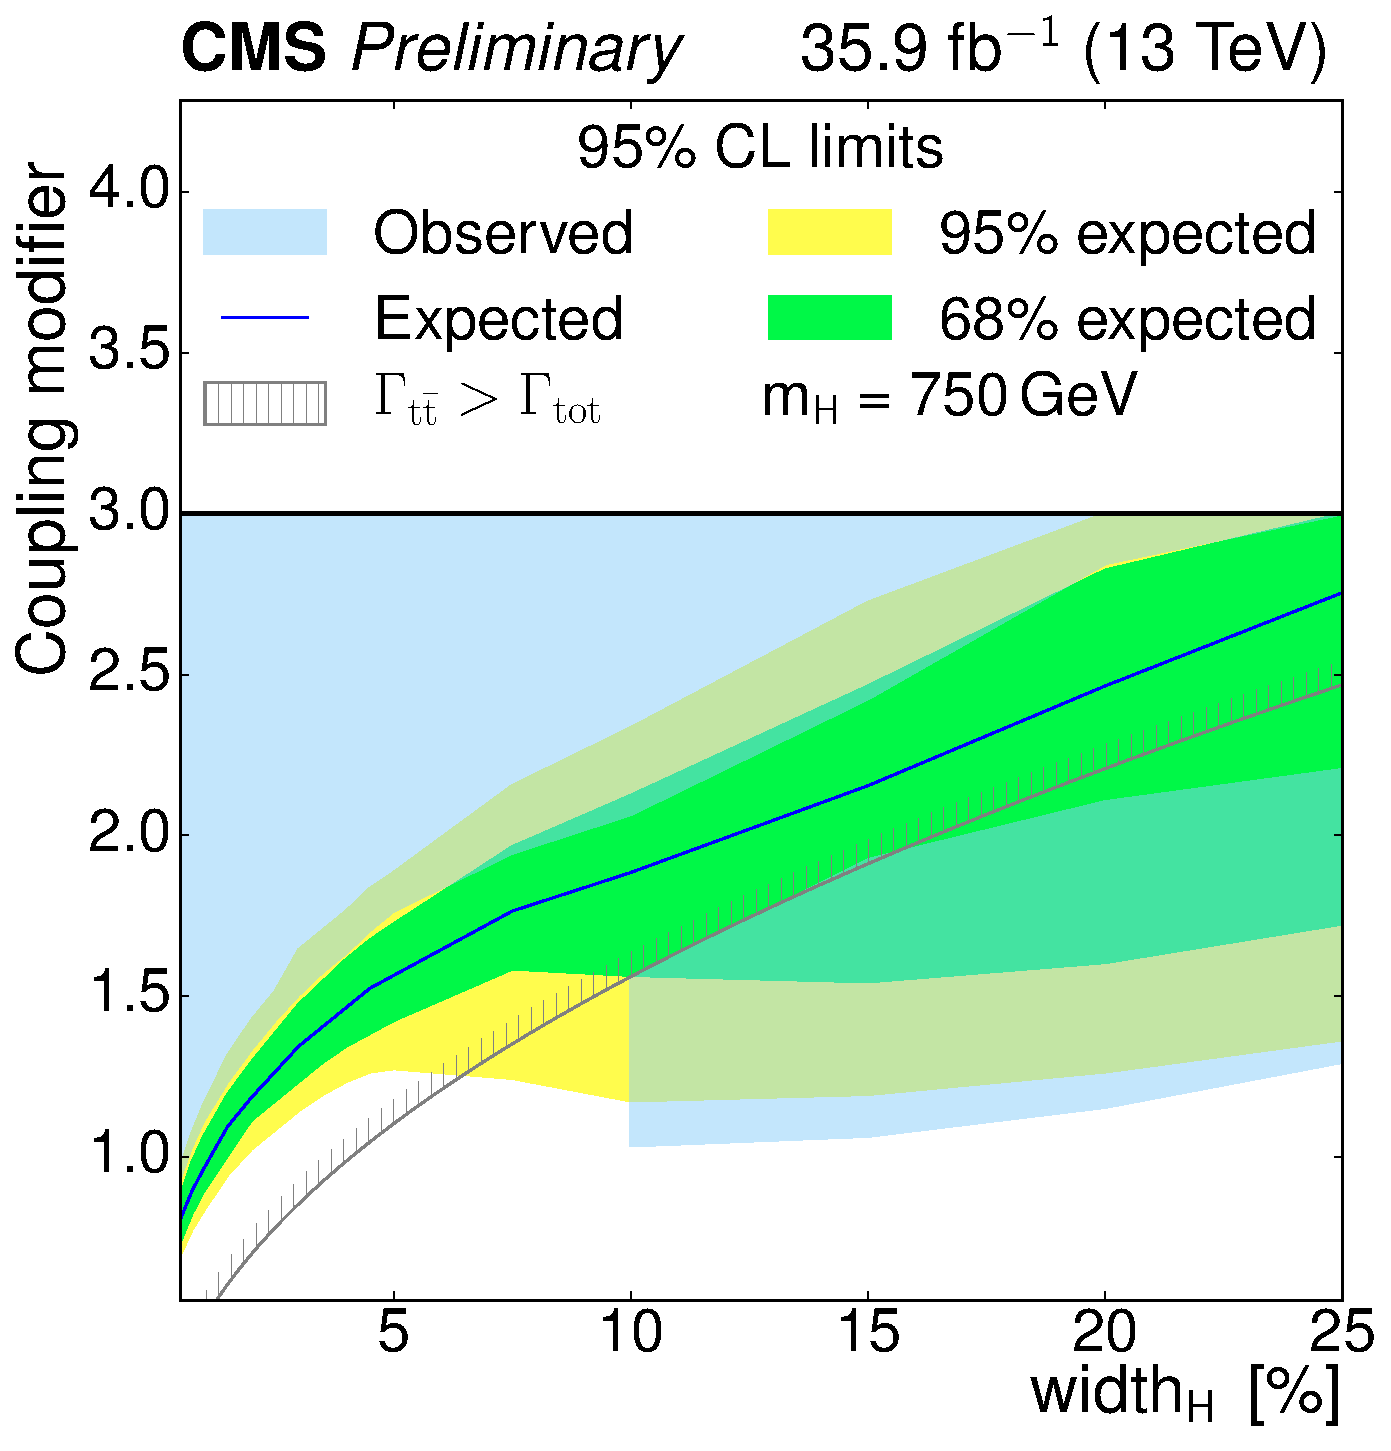
\includegraphics[width=0.35\textwidth,keepaspectratio=true]{fig/chapt8/limits/limit_H_M750.pdf}
\caption{Model-independent combined limits on the coupling strength modifier as a function of relative width for masses between 400 and 750\,GeV in steps of 50\,GeV. The limits are derived for scalar signal only. The observed limits are shown by the blue shaded area. The inner (green) band and the outer (yellow) band indicate the regions containing 68 and 95\%, respectively, of the distribution of limits expected under the background-only hypothesis. The region of phase space in which $\Gamma_{t\bar t}>\Gamma_\mathrm{tot}$ is indicated by the hatched lines.}
\label{fig:limits_h_masses}
\end{figure}

\begin{figure}[!Hhtb]
\centering
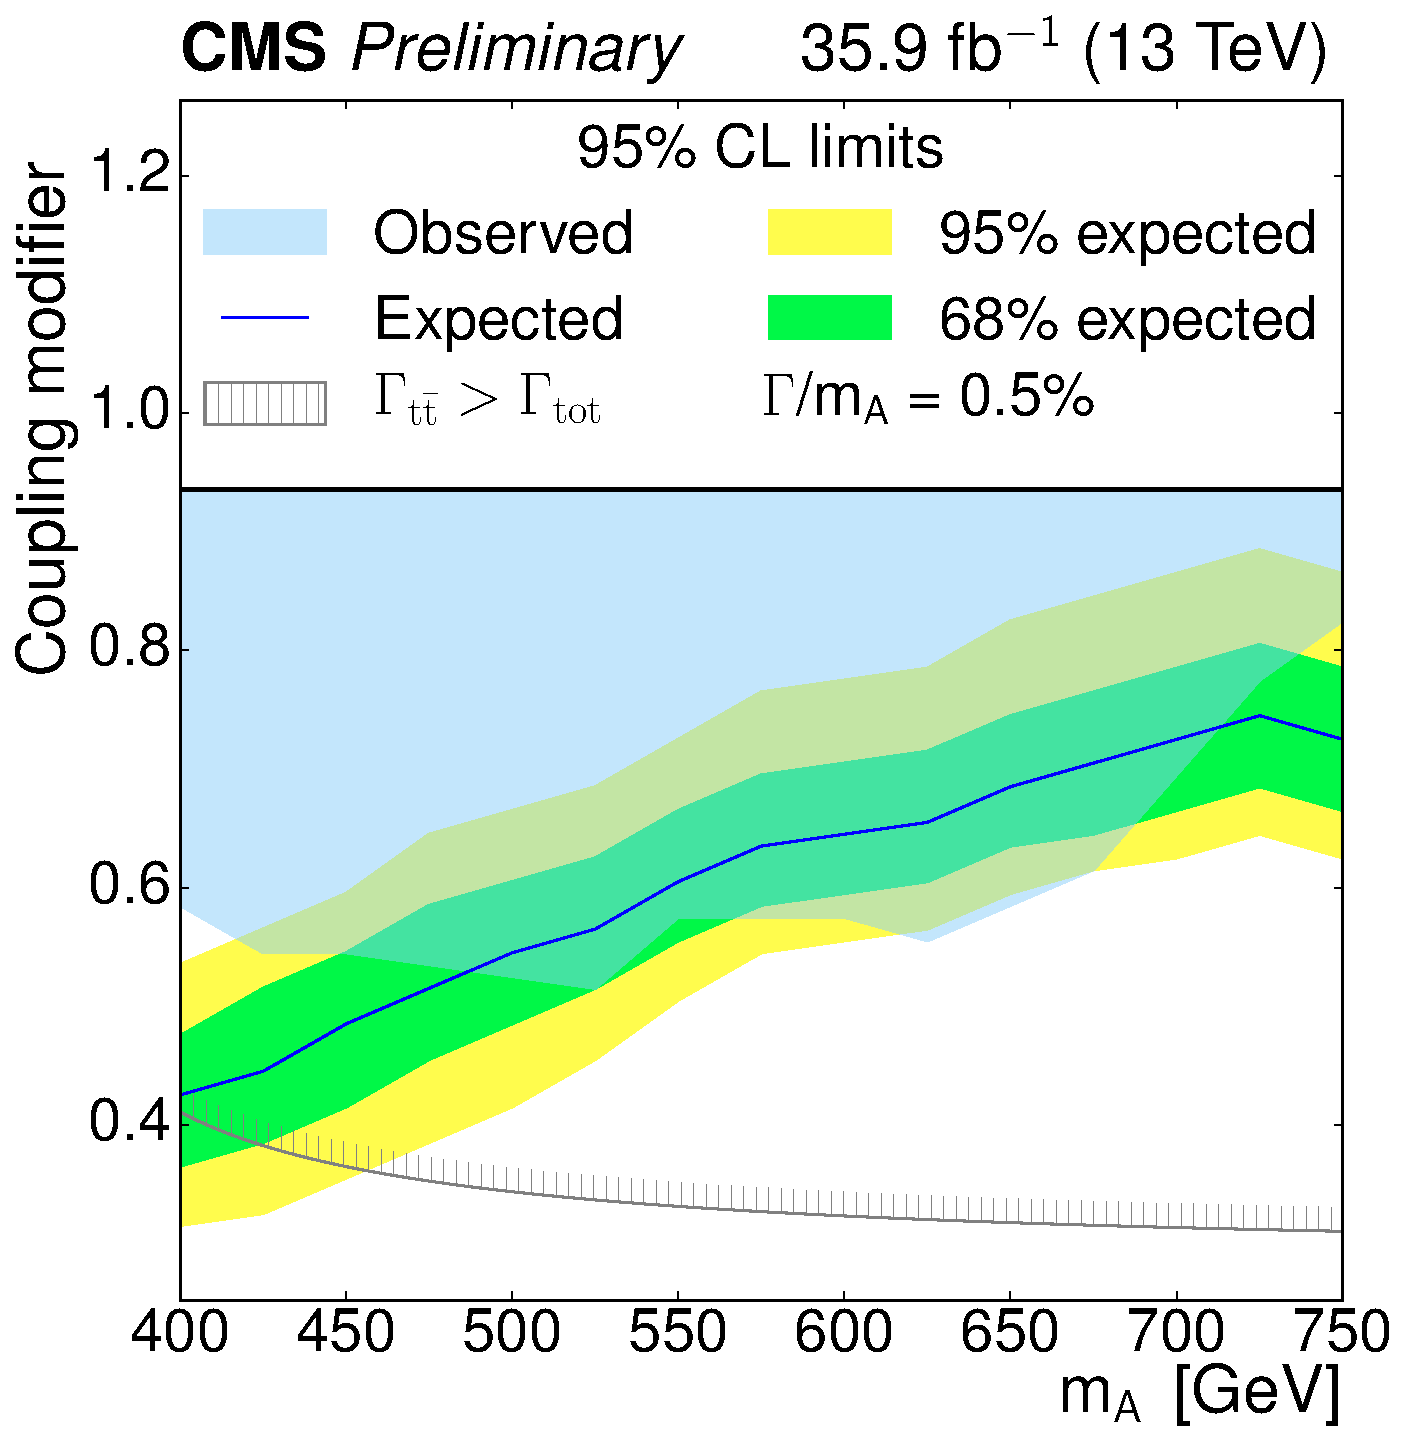
\includegraphics[width=0.35\textwidth,keepaspectratio=true]{fig/chapt8/limits/limit_A_0p5.pdf}
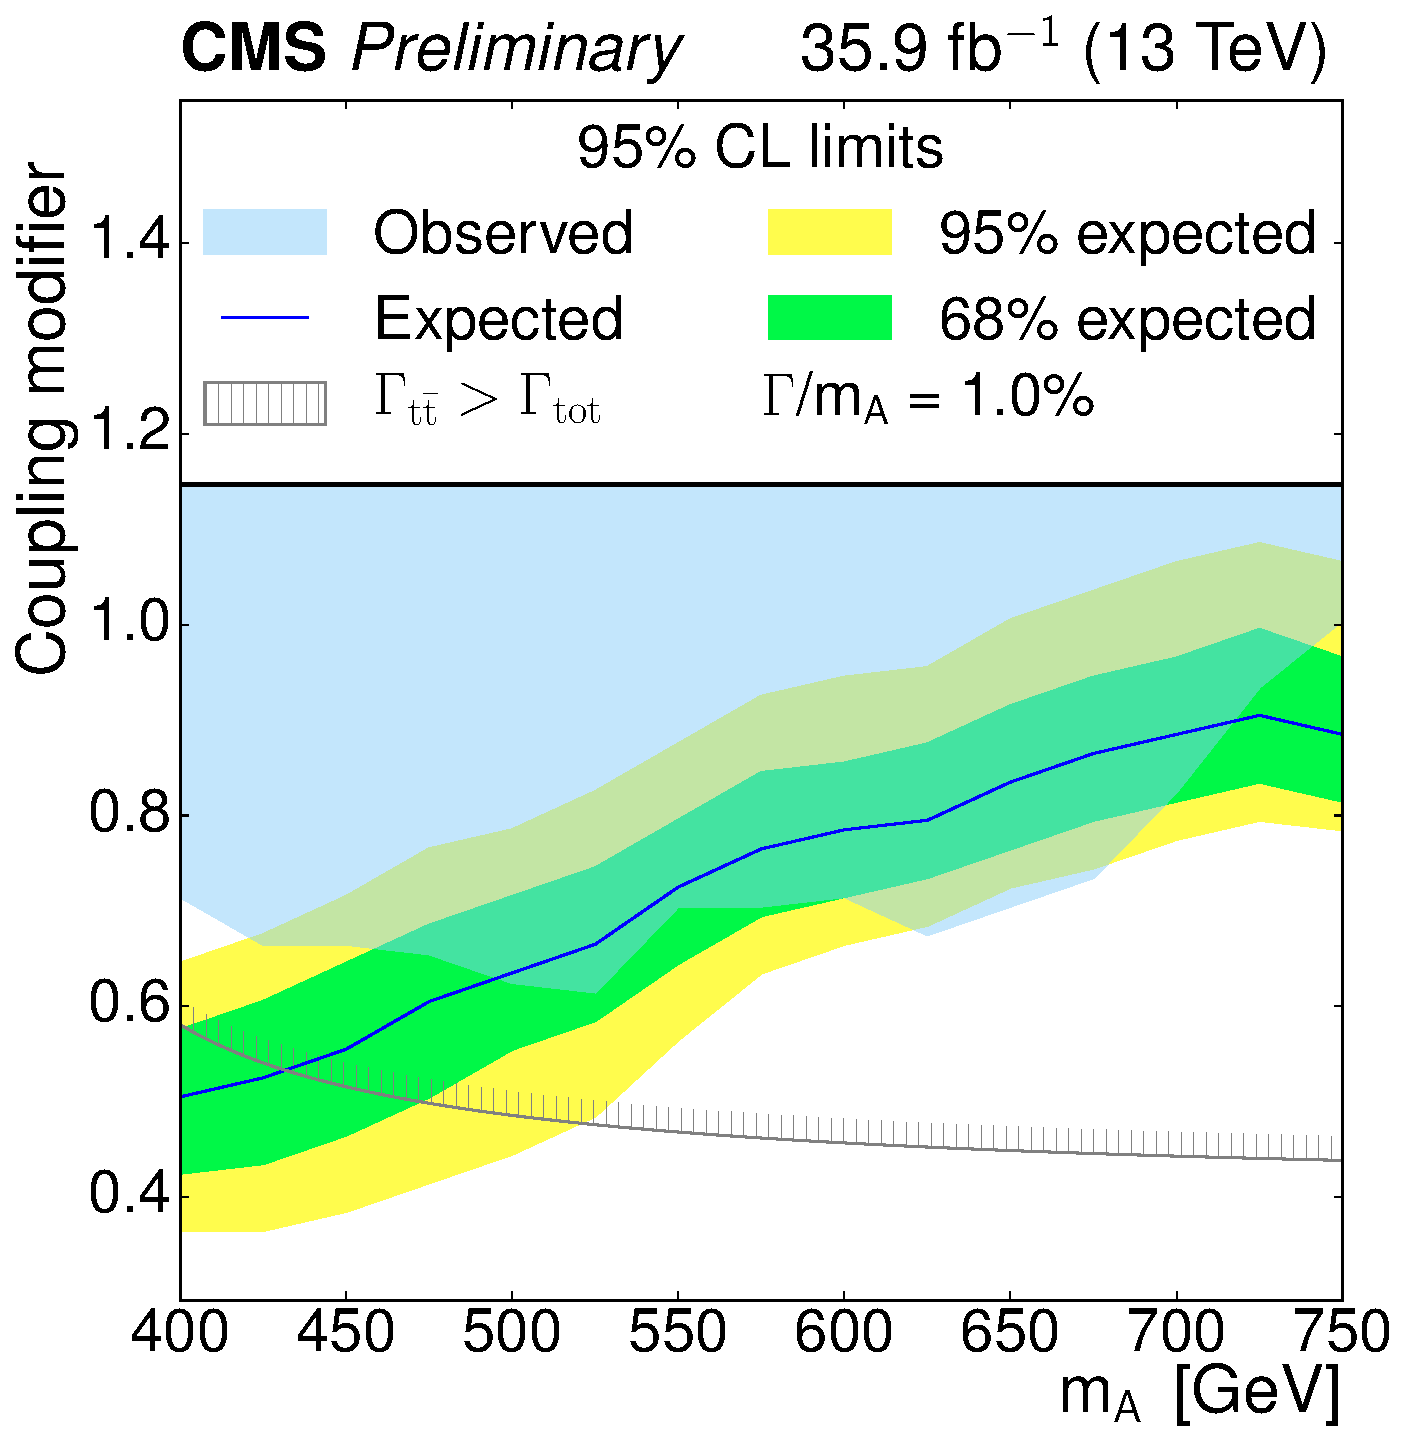
\includegraphics[width=0.35\textwidth,keepaspectratio=true]{fig/chapt8/limits/limit_A_1.pdf}
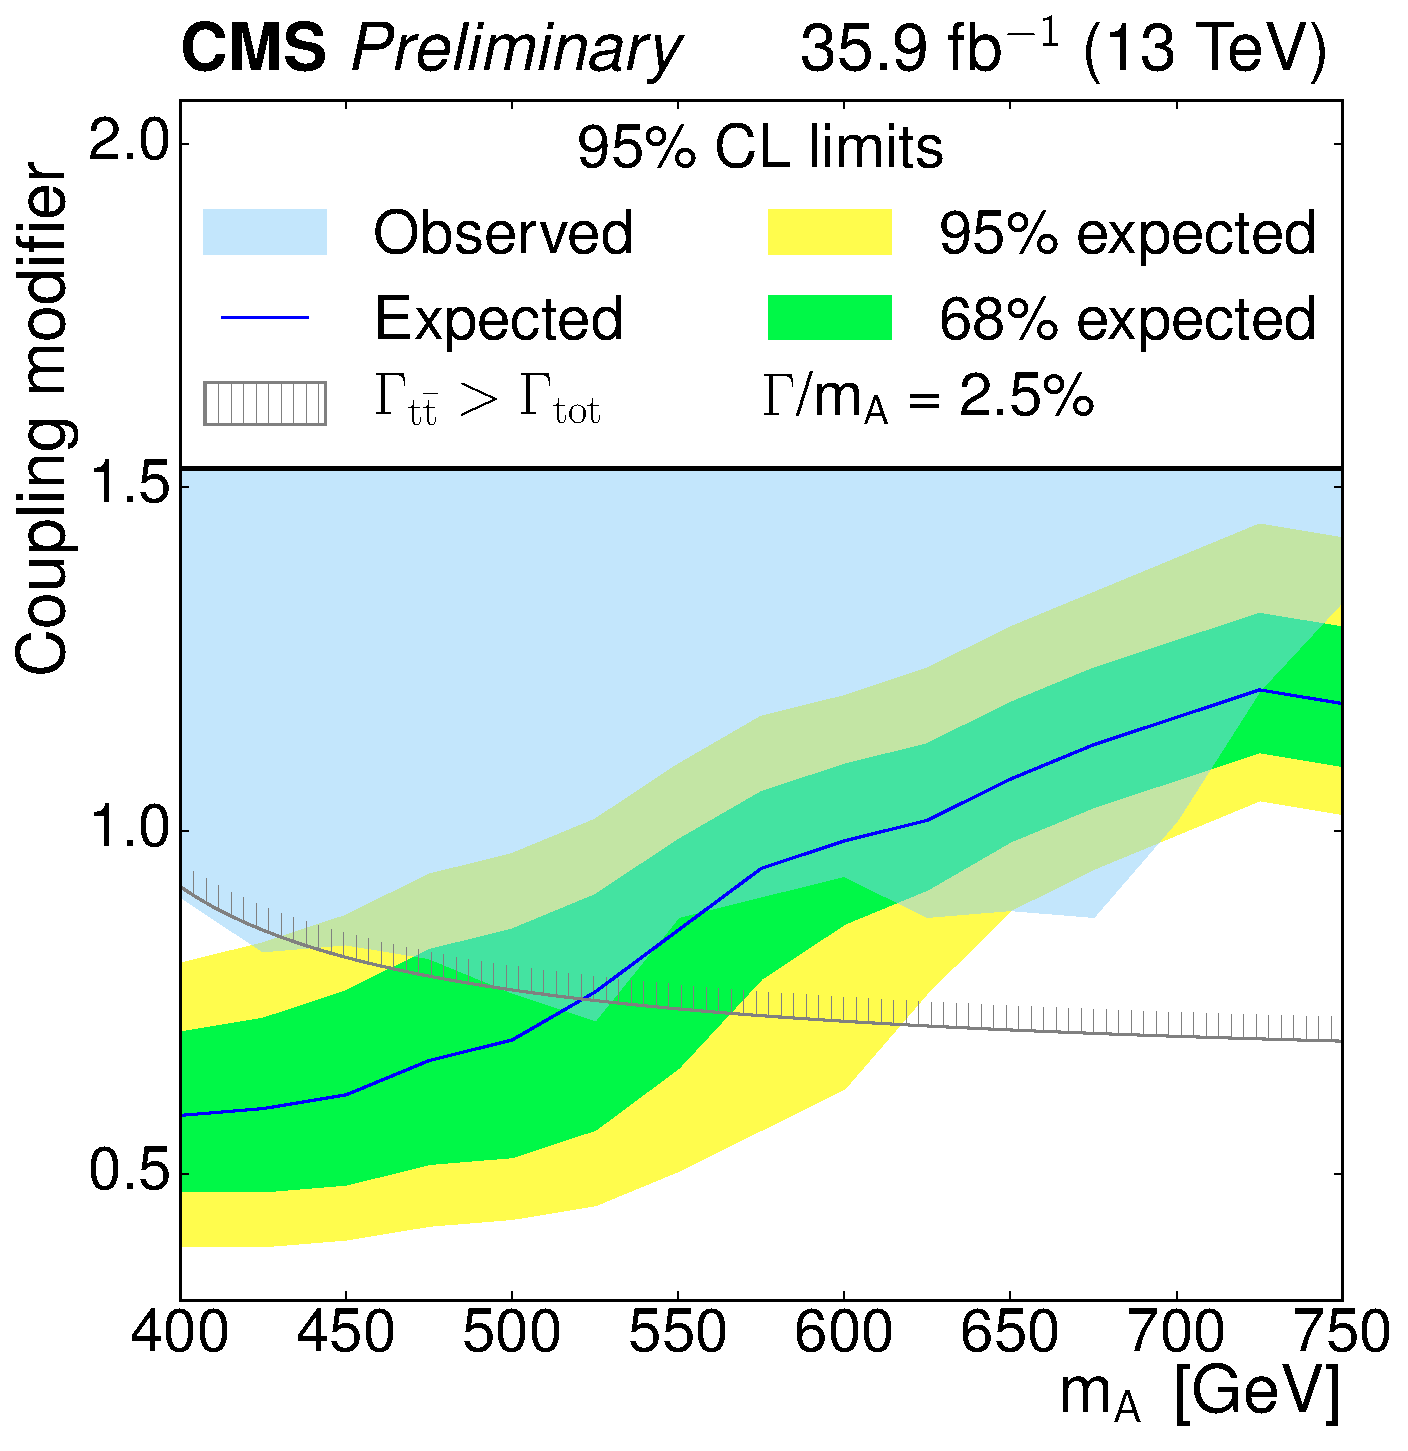
\includegraphics[width=0.35\textwidth,keepaspectratio=true]{fig/chapt8/limits/limit_A_2p5.pdf}
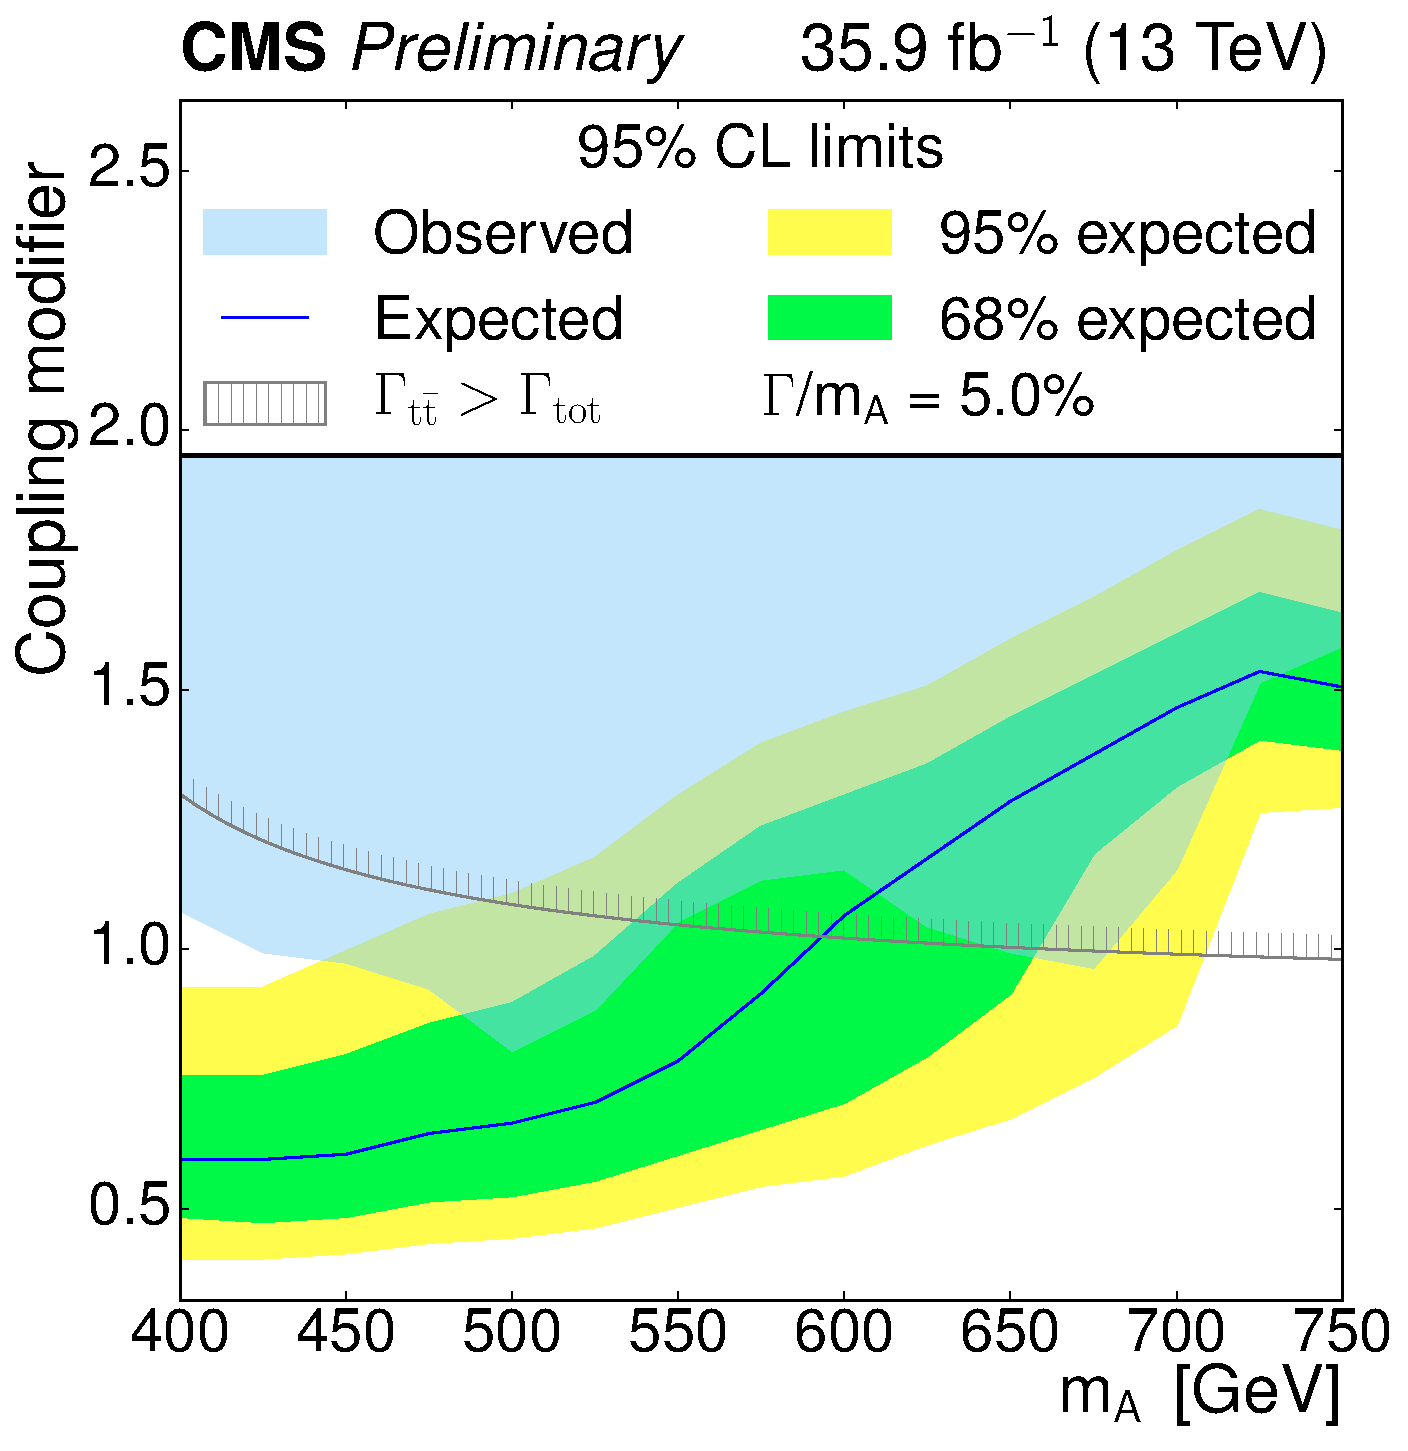
\includegraphics[width=0.35\textwidth,keepaspectratio=true]{fig/chapt8/limits/limit_A_5.pdf}
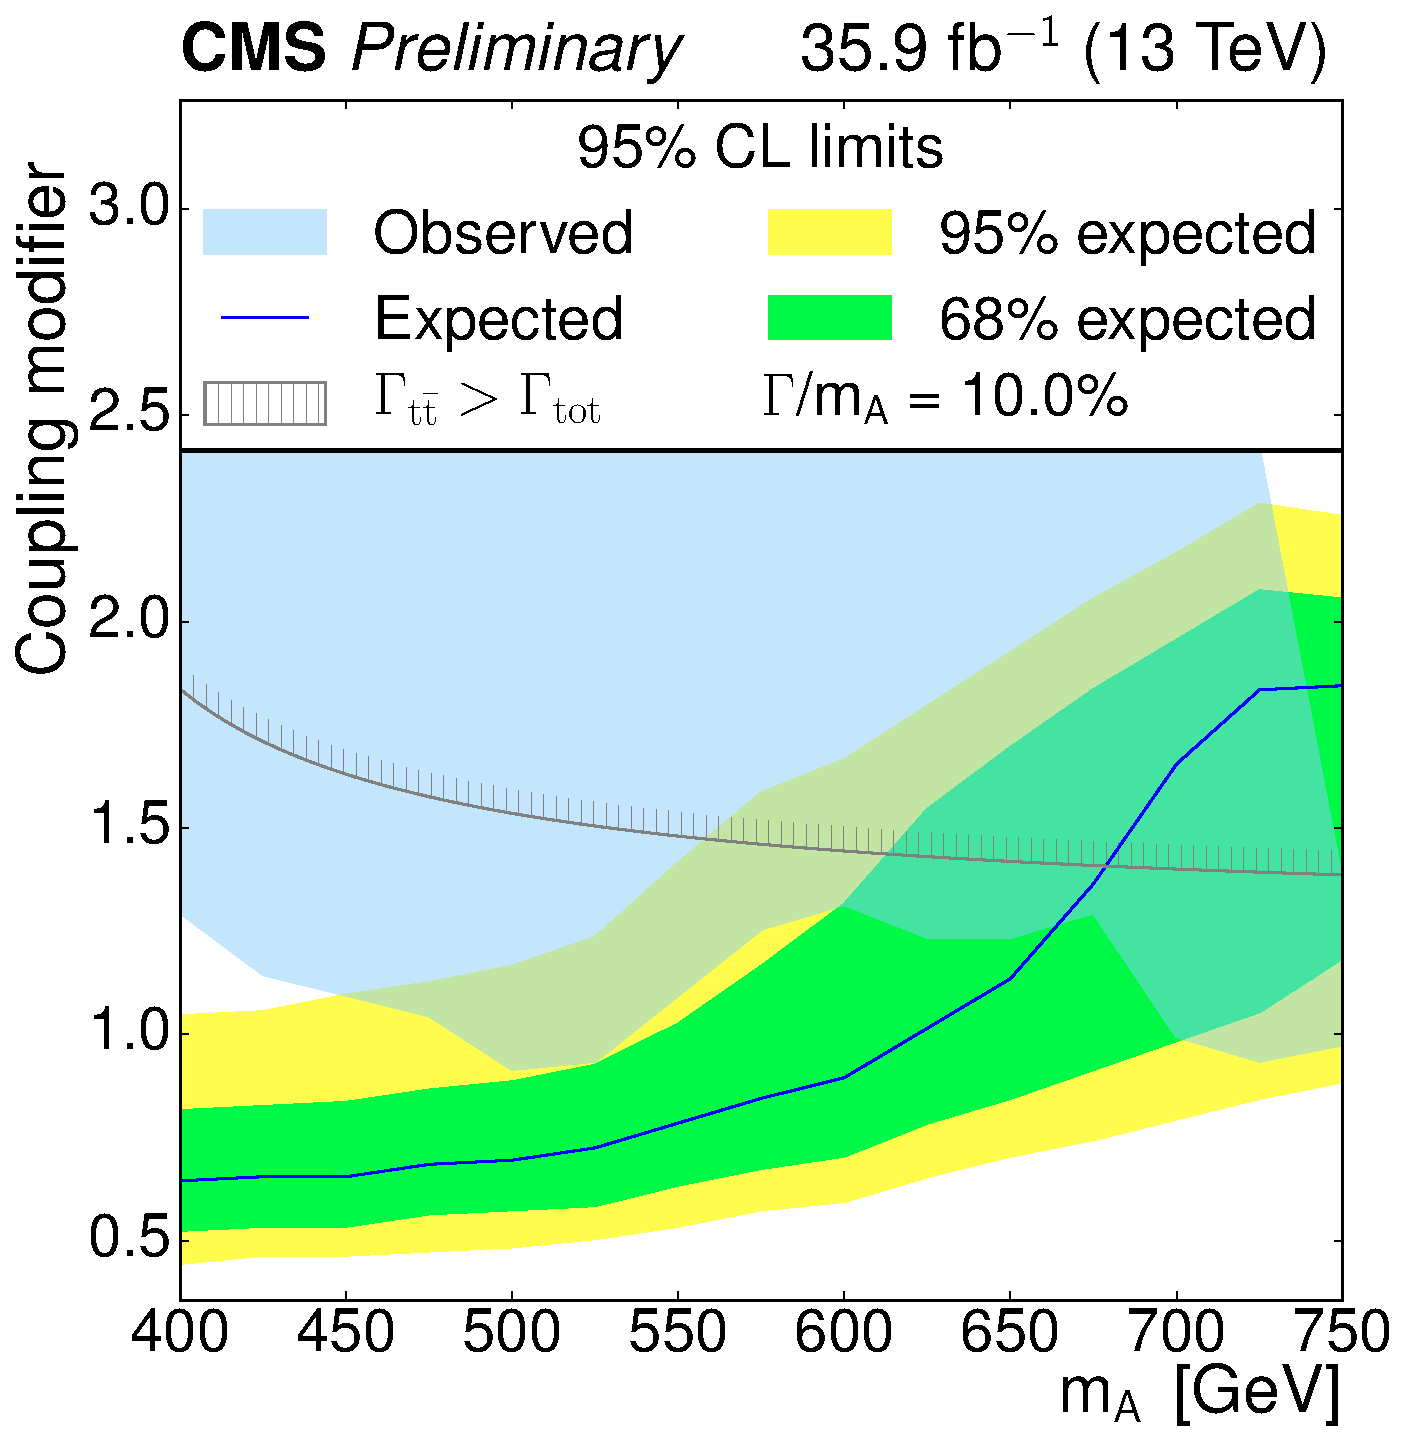
\includegraphics[width=0.35\textwidth,keepaspectratio=true]{fig/chapt8/limits/limit_A_10.pdf}
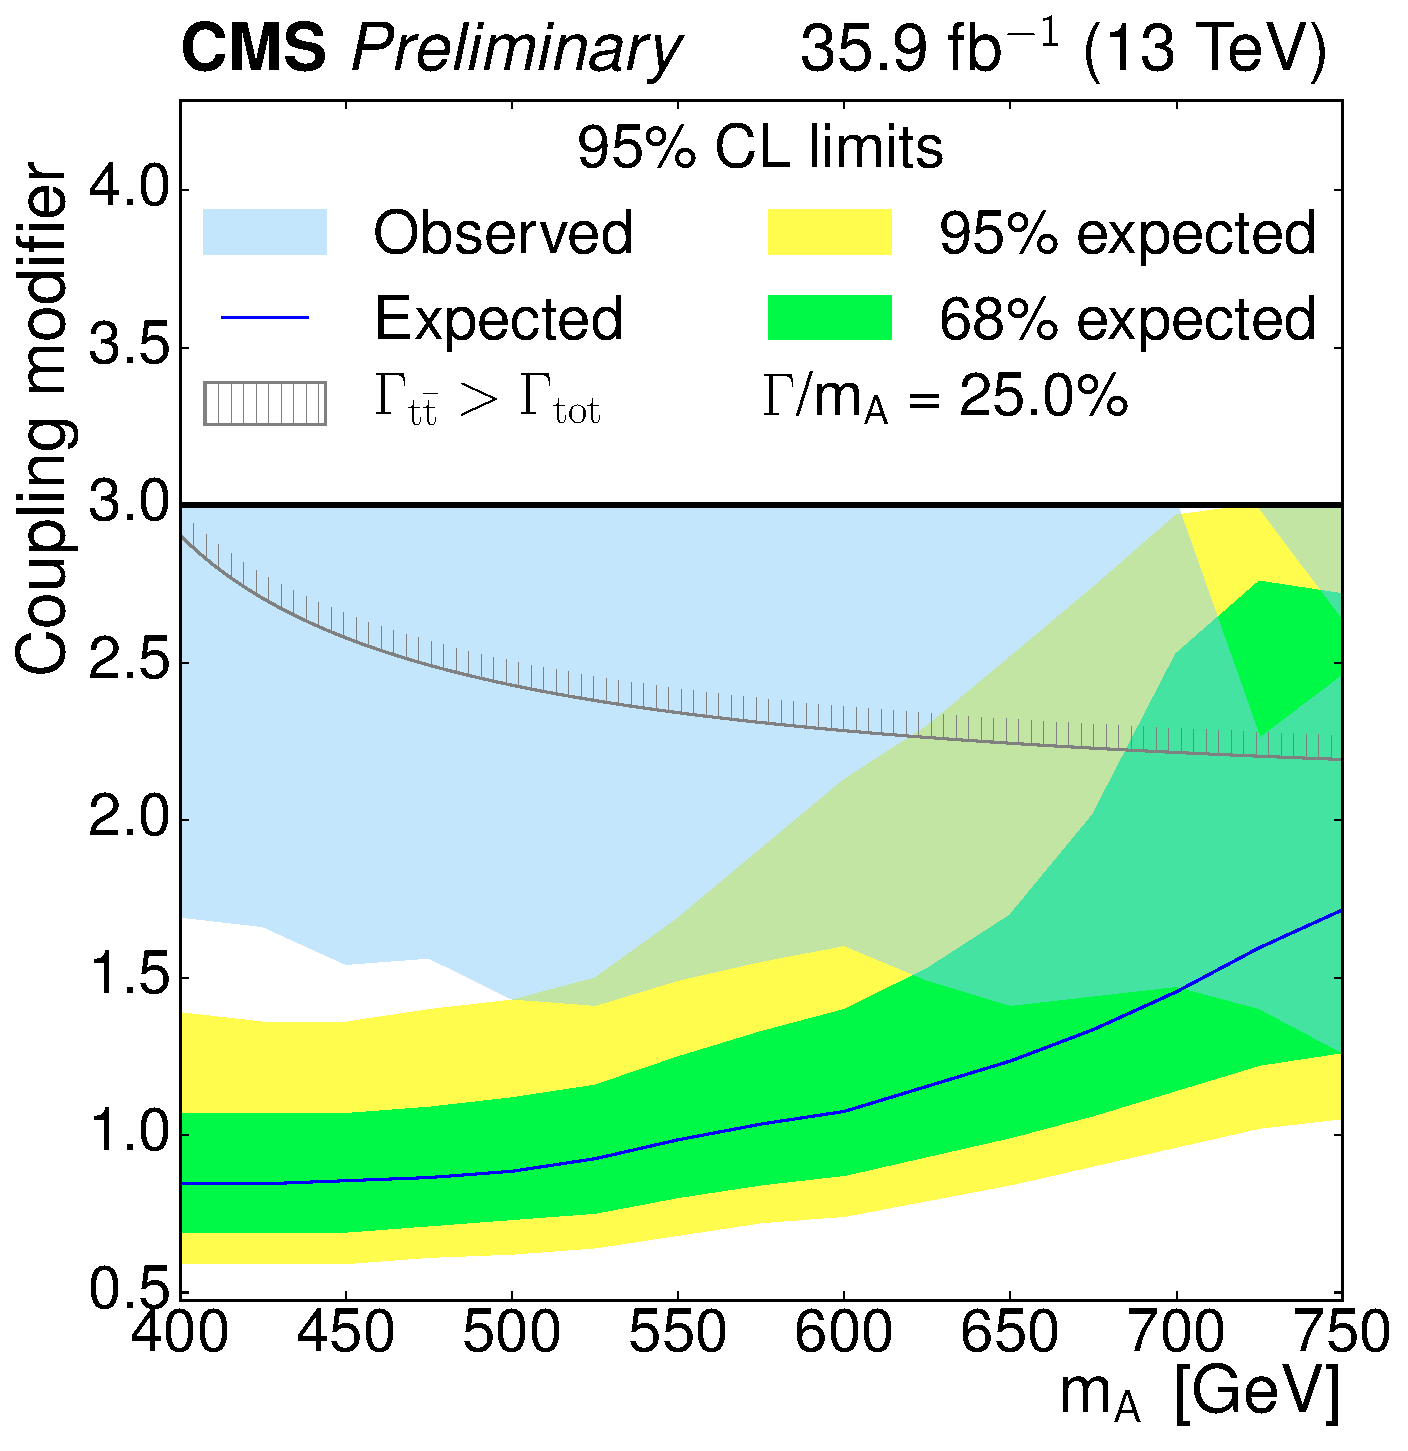
\includegraphics[width=0.35\textwidth,keepaspectratio=true]{fig/chapt8/limits/limit_A_25.pdf}
\caption{Model-independent combined limits on the coupling strength modifier as a function of mass for relative widths of 0.5, 1, 2.5, 5, 10, and 25\%. The limits are derived for pseudoscalar signal only. The observed limits are shown by the blue shaded area. The inner (green) band and the outer (yellow) band indicate the regions containing 68 and 95\%, respectively, of the distribution of limits expected under the background-only hypothesis. The region of phase space in which $\Gamma_{t\bar t}>\Gamma_\mathrm{tot}$ is indicated by the hatched lines.}
\label{fig:limits_a_widths}
\end{figure}

\begin{figure}[!Hhtb]
\centering
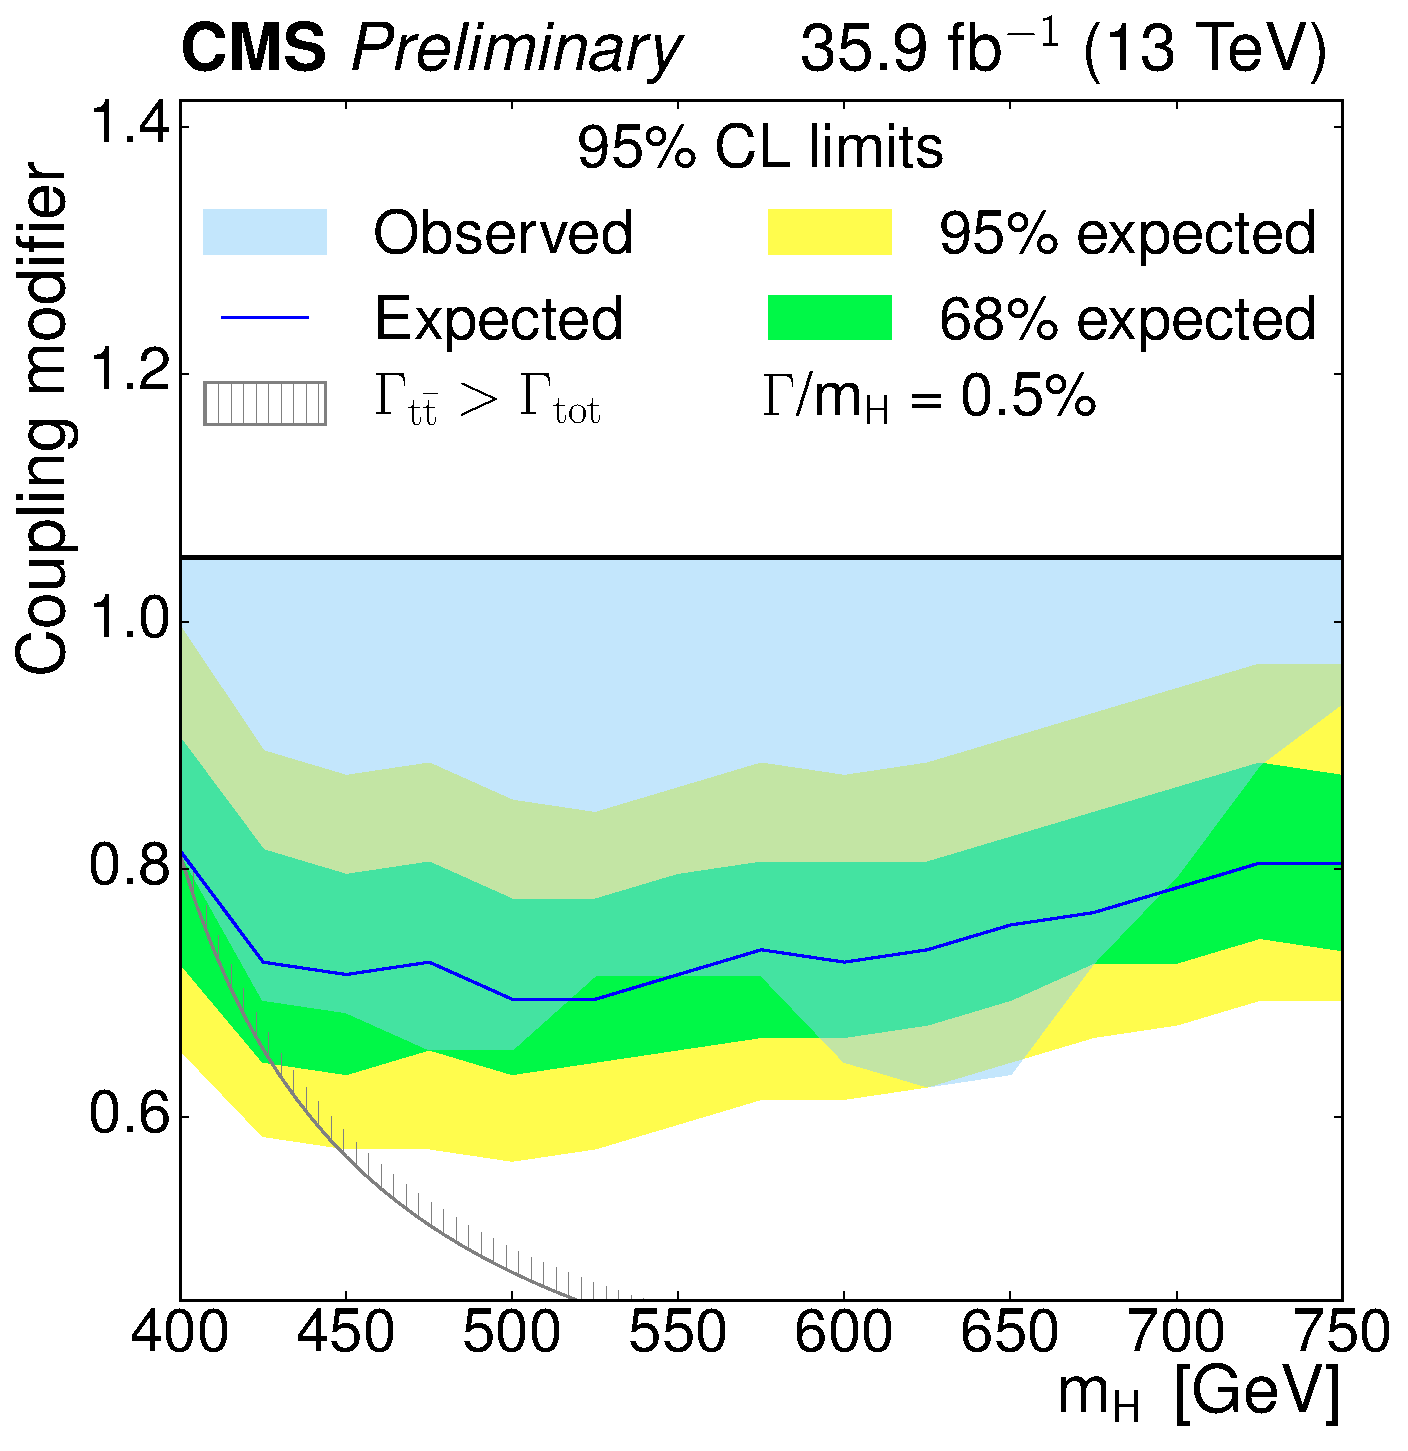
\includegraphics[width=0.35\textwidth,keepaspectratio=true]{fig/chapt8/limits/limit_H_0p5.pdf}
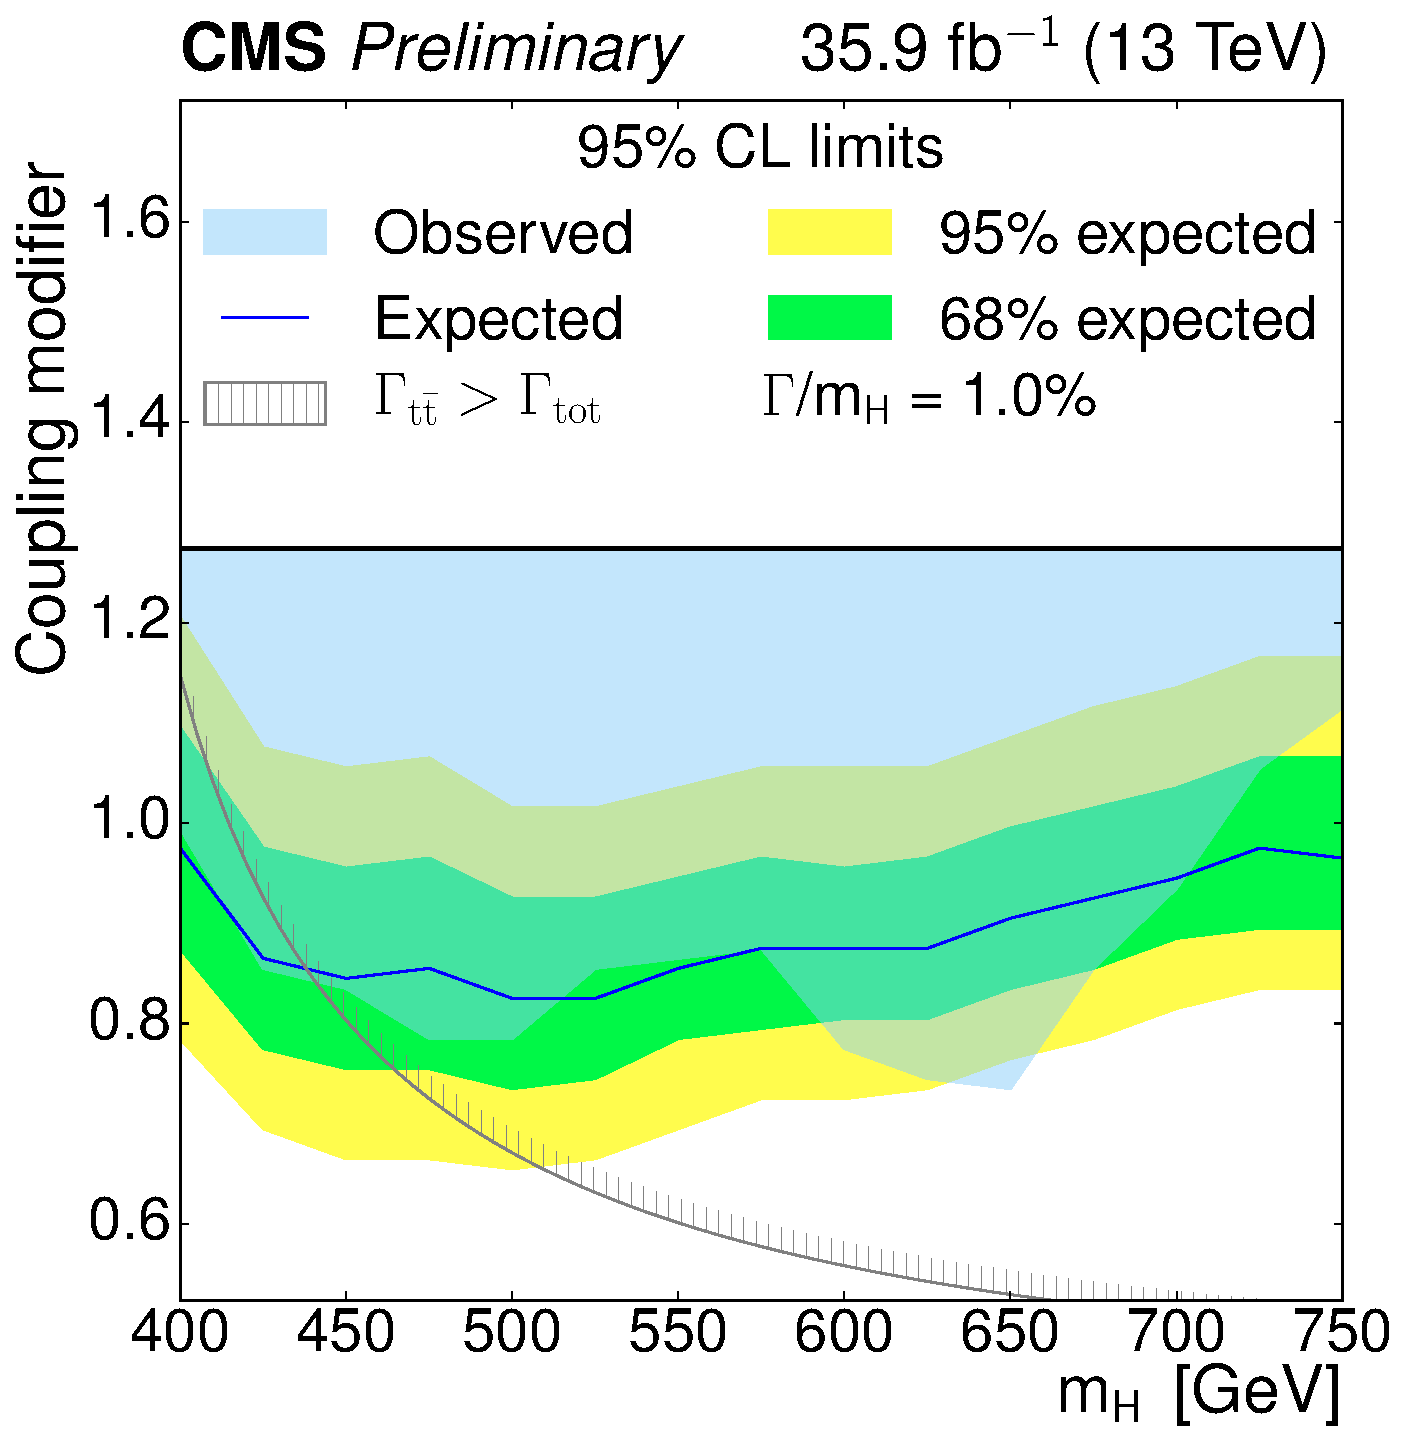
\includegraphics[width=0.35\textwidth,keepaspectratio=true]{fig/chapt8/limits/limit_H_1.pdf}
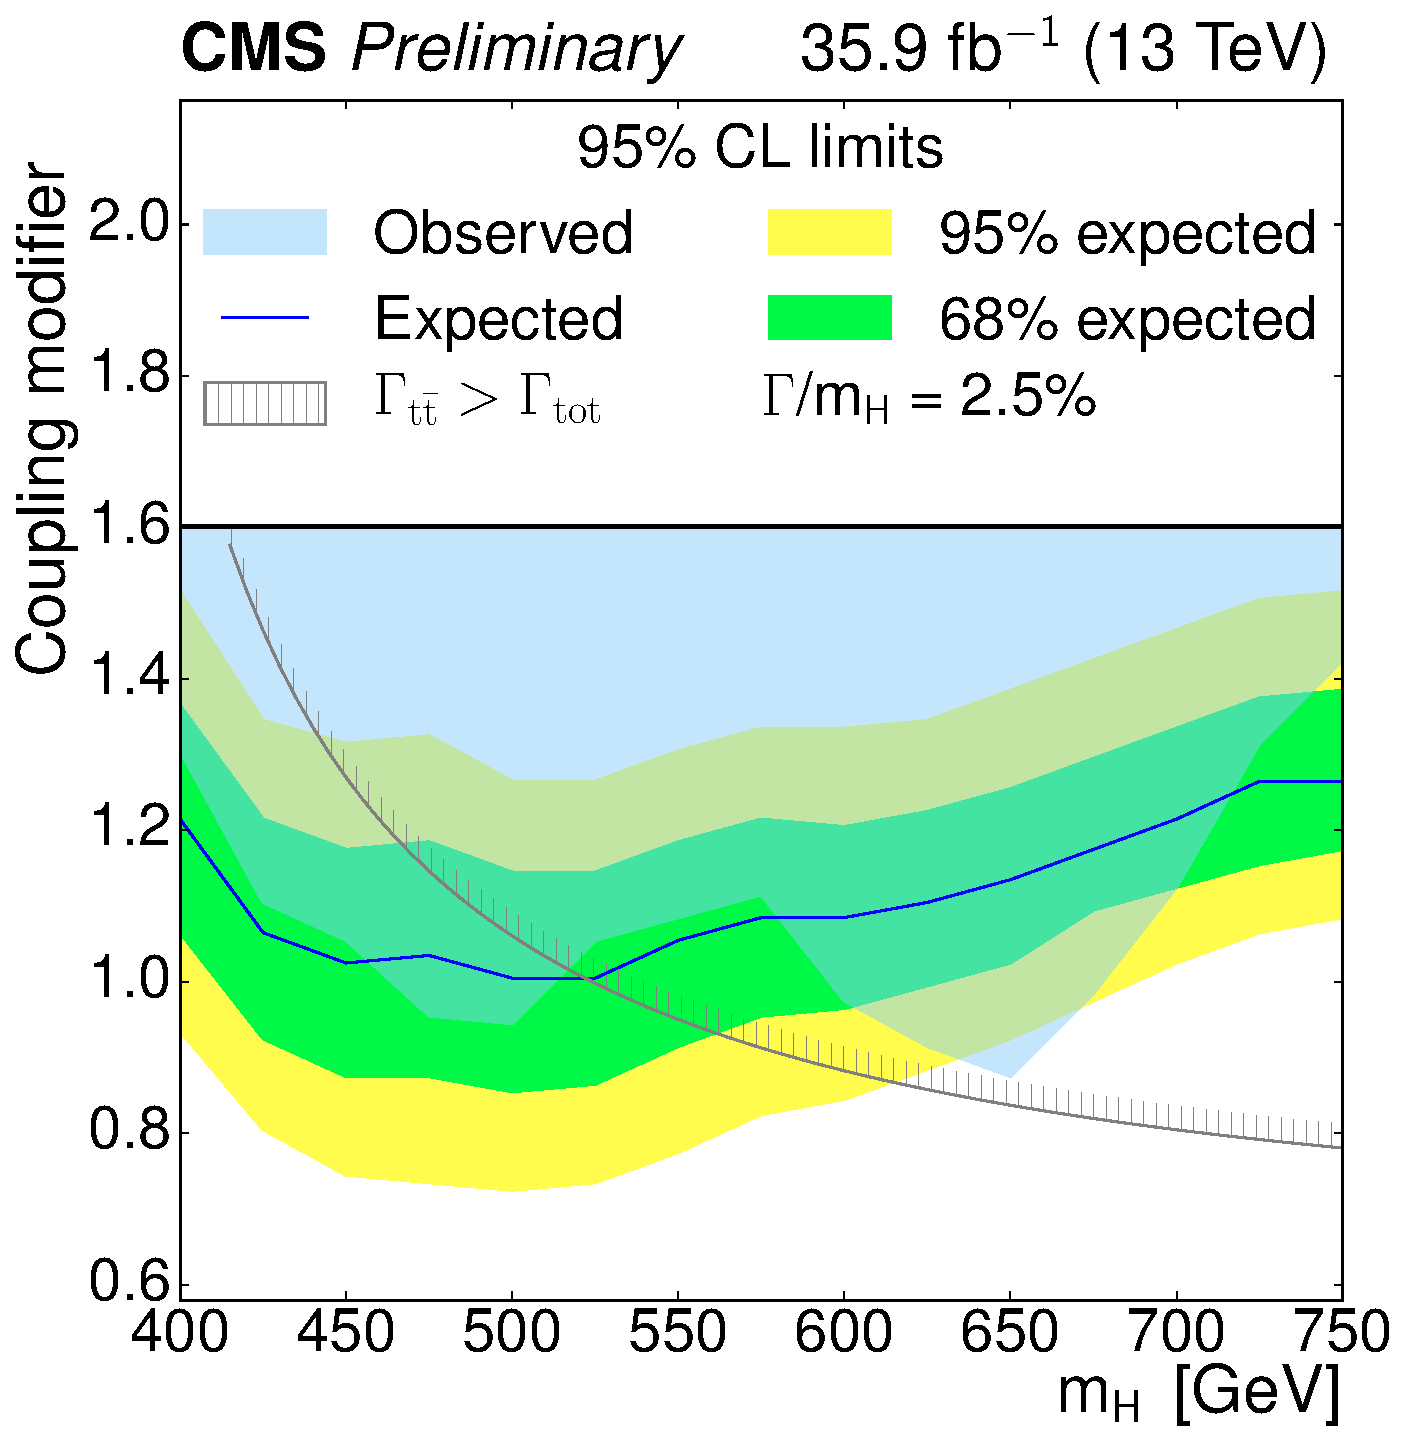
\includegraphics[width=0.35\textwidth,keepaspectratio=true]{fig/chapt8/limits/limit_H_2p5.pdf}
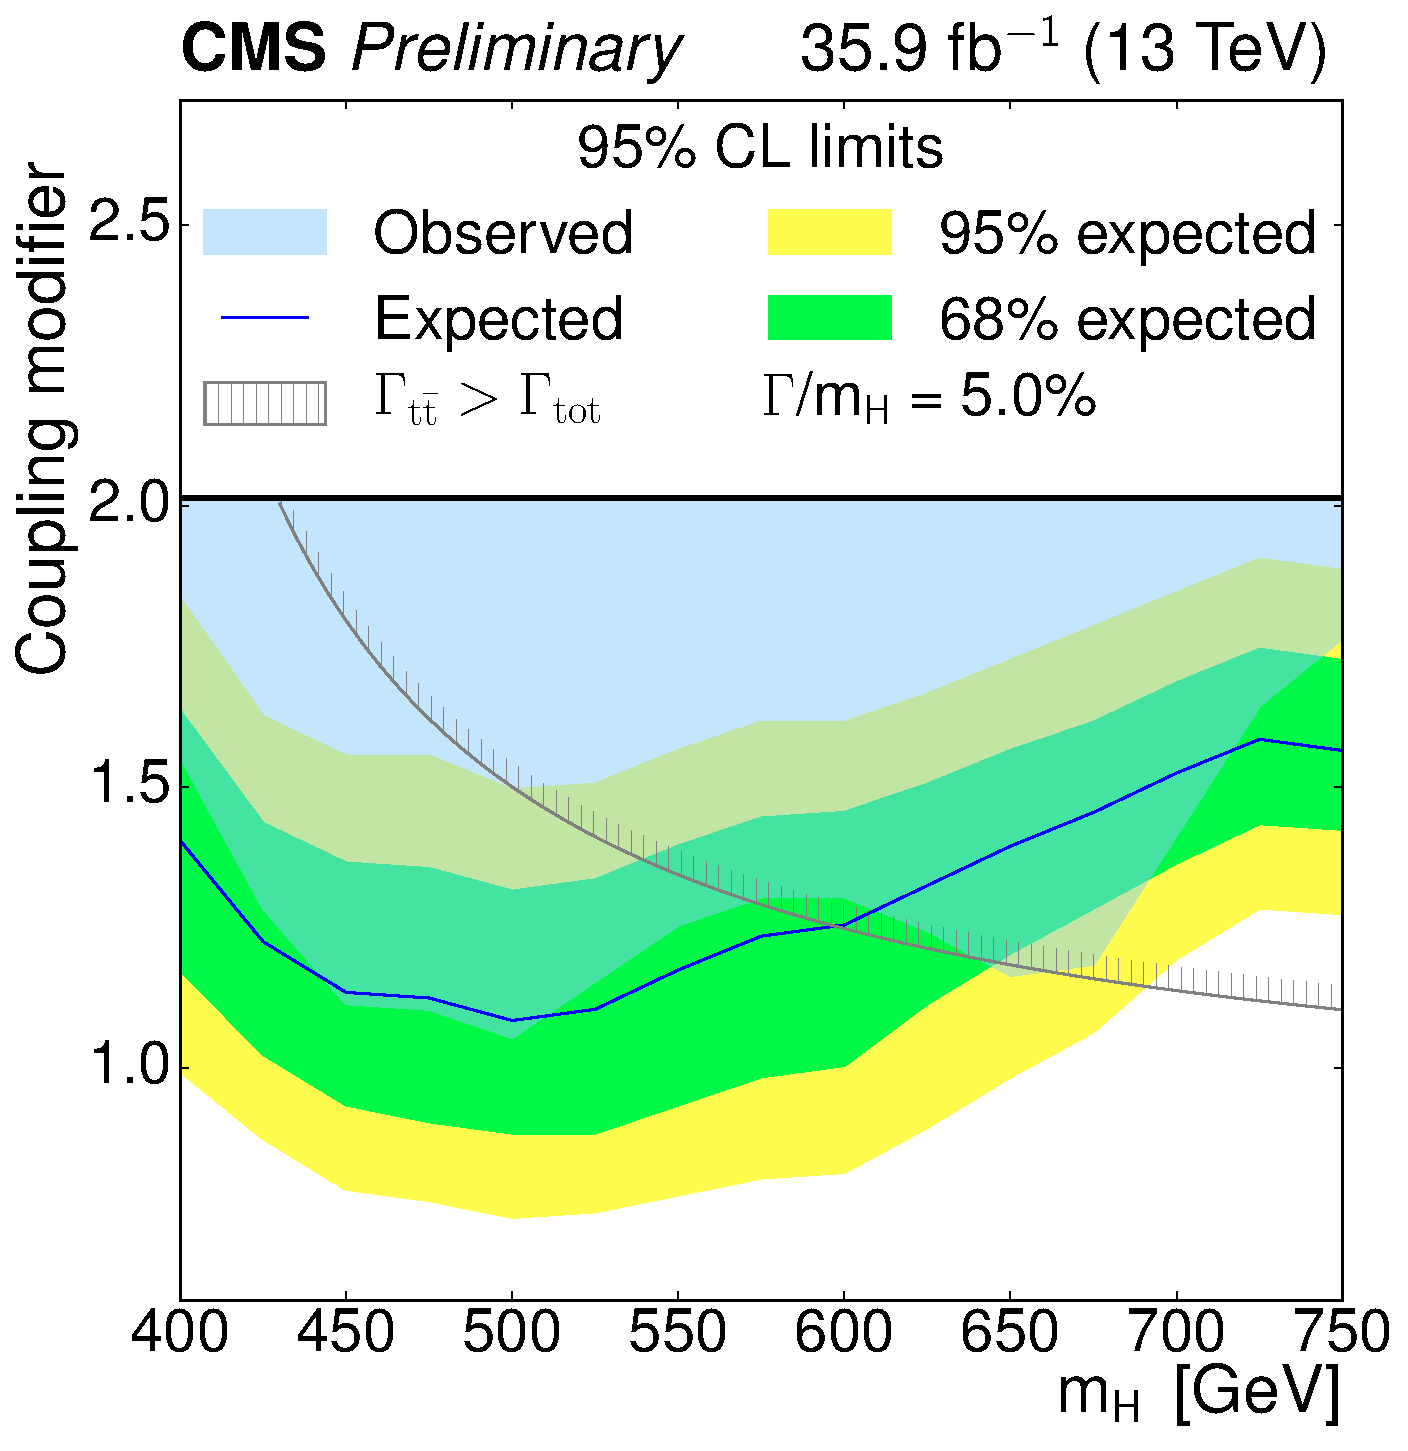
\includegraphics[width=0.35\textwidth,keepaspectratio=true]{fig/chapt8/limits/limit_H_5.pdf}
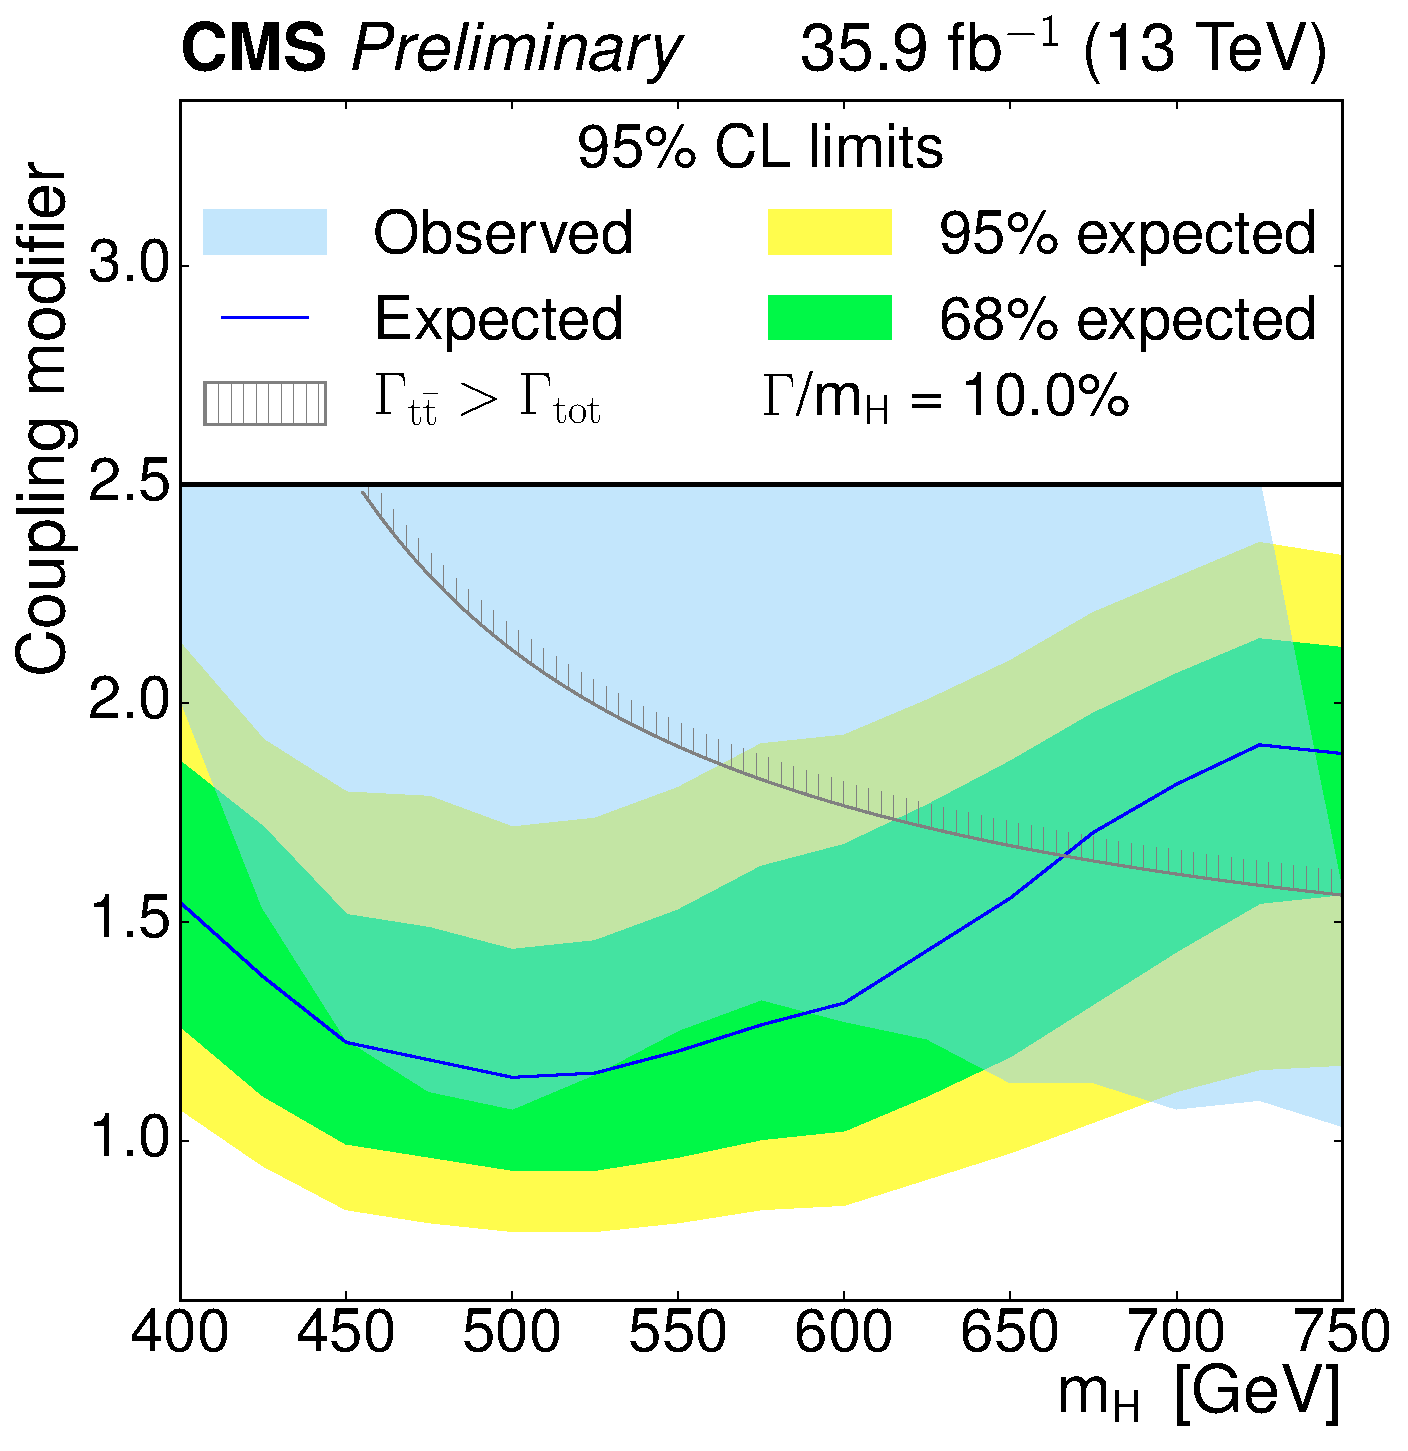
\includegraphics[width=0.35\textwidth,keepaspectratio=true]{fig/chapt8/limits/limit_H_10.pdf}
\includegraphics[width=0.35\textwidth,keepaspectratio=true]{fig/chapt8/limits/limit_H_25.pdf}
\caption{Model-independent combined limits on the coupling strength modifier as a function of mass for relative widths of 0.5, 1, 2.5, 5, 10, and 25\%. The limits are derived for scalar signal only. The observed limits are shown by the blue shaded area. The inner (green) band and the outer (yellow) band indicate the regions containing 68 and 95\%, respectively, of the distribution of limits expected under the background-only hypothesis. The region of phase space in which $\Gamma_{t\bar t}>\Gamma_\mathrm{tot}$ is indicated by the hatched lines.}
\label{fig:limits_h_widths}
\end{figure}

The results are shown in the following figures. All the results are consistent with the SM predictions and no new physics has been observed.

\begin{itemize}
        \item Figure~\ref{fig:limits_a_masses} shows the upper limits for pseudoscalar signal as a function of relative width in bins of mass.
        \item Figure~\ref{fig:limits_h_masses} shows the upper limits for scalar signal as a function of relative width in bins of mass.
        \item Figure~\ref{fig:limits_a_widths} shows the upper limits for pseudoscalar signal as a function of mass in bins of relative width.
        \item Figure~\ref{fig:limits_h_widths} shows the upper limits for scalar signal as a function of mass in bins of relative width.
\end{itemize}


\begin{figure}[!Hhtb]
\centering
\includegraphics[width=0.45\textwidth,keepaspectratio=true]{fig/chapt8/limits/limit_A_2D.pdf}
\includegraphics[width=0.45\textwidth,keepaspectratio=true]{fig/chapt8/limits/limit_H_2D.pdf}
\caption{Model-independent combined upper limits on the coupling strength modifier in the plane of width and either pseudoscalar mass (left) or scalar mass (right). The limits are obtained separately for $A$ production only (left) and for $H$ production only (right).}
\label{fig:limits_h_widths}
\end{figure}

\subsection{Limits in the hMSSM}

Limits in the hMSSM are produced with the following procedure.
First, a grid of points in the $(m_A, \tan\beta)$ plane is produced.
The current setup scans $m_A$ between 400 and 750\,GeV in steps of 50\,GeV,
and $\tan\beta$ beween 0.4 and 10.0 in steps of 0.2.
The lower limit on $\tan\beta$ of 0.4 is imposed to guarantee that the amplitudes preserve perturbative unitarity for all calculations.

For each such-produced $(m_A, \tan\beta)$ pair, the corresponding values of $m_H$ and the widths of the $A$ and $H$ bosons are obtained with 2HDMC~\cite{2hdmc}.
With the help of mass morphing and width interpolation/extrapolation where necessary, templates are constructed that correspond to the mass and width values obtained.
With the such obtained templates, upper limits on the coupling strength modifier are calculated as outlined above.
If the obtained limit on the coupling strength is smaller than the coupling strength that corresponds to the given $\tan\beta$, i.e.\ $g = 1/\tan\beta$, the given point is excluded.
The $\pm 1$ and $\pm 2\sigma$ bands of the expected limits are extracted in the same way.

\begin{figure}[!Hhtb]
\centering
\includegraphics[width=0.9\textwidth,keepaspectratio=true]{fig/chapt8/limits/hmssm_exclusion.pdf}
\caption{95\% confidence level limits on $(m_A, \tan\beta)$ in the hMSSM, using the combination of all channels and including both $A$ and $H$ signals with the masses and widths that correspond to a given point in the ($m_A, \tan\beta$) plane.}
\label{fig:limits_hmssm}
\end{figure}

Figure~\ref{fig:limits_hmssm} shows the such-obtained limits in the $(m_A, \tan\beta)$ plane.
The expected upper limits on $\tan\beta$ range from 2.3 at $m_A = 400\,GeV$ to 0.5 at $mA = 700\,GeV$.
These are the first experimental limits in the region of low $\tan\beta$ and $m_A$ beyond the $t\bar t$ production.
The presented search hence gives access to a new region of phase space in searches for additional Higgs bosons in the MSSM context.
While the presented results use the strict mass relations in the MSSM, they can easily be translated to more generic type-2 2HDM models.

\section{Summary}

Results of the combination of searches for additional Higgs bosons decaying to $t\bar t$ are presented.
Upper limits are placed on the coupling modifer of these additional Higgs bosons to top quarks.
These upper limits are given in a model-independent way in terms of the masses and widths of the either scalar or pseudoscalar new particles.
In addition, the results are interpreted in the hMSSM (minimal supersymmetric standard model), which is an example of a two-Higgs doublet model of type 2 and considers the lightest additional scalar to correspond to the 125\,GeV Higgs boson observed by the ATLAS and CMS experiments.
Limits are given in the $(m_A, \tan\beta)$ plane.
This analysis is sensitive in the low $\tan\beta$ region and has complementary sensitivity to previous searches, which are either sensitive at high $\tan\beta$ (di-tau final state) or for masses below the $t\bar t$ production threshold~\footnote{in particular searches for di-Higgs boson production and for pseudoscalars decaying to the 125\,GeV Higgs boson and a $Z$~boson, and constraints from the observed couplings of the 125\,GeV Higgs boson}.


\clearpage{\pagestyle{empty}\cleardoublepage}

\renewcommand*{\thesection}{\thechapter.\arabic{section}}       % reset again to chaptnum.sectnum


